\documentclass[platex,dvipdfmx,10.5pt,a4j]{jarticle}
\usepackage{setspace}
\usepackage{url}
\usepackage[dvipdfmx]{graphicx}
\usepackage{float}
\usepackage{fancyhdr}
\usepackage[title]{appendix}
\usepackage{amsmath}
\usepackage{multirow}
\usepackage{bm}
\usepackage{amssymb}
\usepackage{tocloft}

\makeatletter
	\renewcommand{\theequation}{% 式番号の付け方
	\thesection.\arabic{equation}}
	\@addtoreset{equation}{section}

	\renewcommand{\thefigure}{% 図番号の付け方
	\thesection.\arabic{figure}}
	\@addtoreset{figure}{section}

	\renewcommand{\thetable}{% 表番号の付け方
	\thesection.\arabic{table}}
	\@addtoreset{table}{section}
\makeatother

% Abstractの書式設定
% 参考:https://tex.stackexchange.com/questions/366169/how-to-change-font-size-for-abstract-title
\makeatletter
\renewenvironment{abstract}{%
    \if@twocolumn
      \section*{\abstractname}%
    \else
      \begin{flushleft}%
        {\bfseries \LARGE\abstractname\vspace{\z@}}
      \end{flushleft}%
      \quotation
    \fi}
    {\if@twocolumn\else\endquotation\fi}
\makeatother

\renewcommand{\cfttoctitlefont}{\LARGE}

\renewcommand{\figurename}{Fig}
\renewcommand{\tablename}{Table}
\renewcommand{\refname}{参考文献}
\renewcommand{\abstractname}{Abstract}

\begin{document}
\begin{center}

    \begin{spacing}{4}
        \vspace{\baselineskip}
    \end{spacing}

    \begin{spacing}{2}
        {\Huge \underline{機能デザイン研究I\hspace{-.1em}I}}
    \end{spacing}

    \begin{spacing}{2}
        \vspace{\baselineskip}
    \end{spacing}

    {\Large 令和2年2月9日提出}

    \begin{spacing}{2}
        \vspace{\baselineskip}
    \end{spacing}

    \vskip 5.8zh
    \[ \left. \begin{array}{ll}
            \mbox{{\Large 杉山 和靖}} & \mbox{{\Large 教授}} \\
            \mbox{{\Large 渡村 友昭}} & \mbox{{\Large 助教}}
        \end{array} \right\} \mbox{{\large 指導}}
    \] \par
    \vskip 5.3zh

    \begin{spacing}{2}
        \vspace{\baselineskip}
    \end{spacing}

    \begin{spacing}{1.2}
        {\Large 大阪大学大学院基礎工学研究科}
    \end{spacing}
    \begin{spacing}{1.2}
        {\Large 機能創成専攻機能デザイン領域}
    \end{spacing}
    \begin{spacing}{1.2}
        {\Large 推進工学講座}
    \end{spacing}
    \begin{spacing}{1.2}
        {\Large 29B20038}
    \end{spacing}
    \begin{spacing}{1.5}
        \vspace{\baselineskip}
    \end{spacing}
    \begin{spacing}{1.2}
        {\Large 丹羽 英人}
    \end{spacing}
\end{center}

\newpage
\thispagestyle{empty}
\begin{abstract}
ここにアブストを書く
\end{abstract}
\newpage
\setcounter{page}{1}
\setcounter{tocdepth}{2}
\tableofcontents
\newpage
\pagestyle{fancy}
\rhead{}
\lhead{\rightmark}
\cfoot{\thepage}
\rfoot{}
\renewcommand{\footrulewidth}{0.4pt}
\renewcommand{\headrulewidth}{0.4pt}

\section{緒言}

\subsection{研究背景}

一般的に,流体はせん断応力がせん断速度に比例するNewton流体と,せん断応力がせん断速度が非線形となる非Newton流体に分類することができる.

Fig.\ref{fig:1-fluid-curve}(a)に示す通り,Newton流体はせん断速度とせん断応力が比例関係にある流体である.一方でそれ以外の流体は非Newton流体と呼ばれている.非Newton流体はDilatant fluid, Pseudoplastic, Bingham plastic, Viscoplastic, Viscoelastic が挙げられている.
非Newton流体のうち,Bingham plastic 流体, Viscoplastic 流体はせん断応力がある一定になるまでせん断速度が発生しない流体である.一方で,Dilatant fluid 流体, Pseudoplastic 流体はせん断応力が少しでも加わると,せん断速度が発生し流体的挙動を示す.また,Viscoelastic 流体は粘性だけでなく弾性的挙動を示す流体である.これら非Newton流体の粘度を示す理論として,Power-law model (Ostwald-De Waele model), Cross model,Carreau model,Carreau-Yasuda modelやHerschel-Bulkley modelなどを挙げることができる\cite{ref:1}.Power-law model はせん断速度の限られた範囲内にて適応することができる.理論式中の指数によってNewton流体,shear-thinning流体と,shear-thickening流体に分類することができる.これらのせん断速度と粘度の関係性はFig.\ref{fig:1-fluid-curve}(b)に示す通りである.これら2種類の流体のうち,本研究で扱うshear-thinning流体は,せん断速度$\dot{\gamma}$が高くなるほど粘度$\mu$が低くなる性質を有している.この流体は擬塑性流体とも呼ばれている.擬塑性流体の代表例として,泥や血液,ポリマーなどが挙げられる.本研究において試験溶液としたポリマーの流動は,粘性だけでなく弾性にも依存する\cite{viscoelasticity}.産業分野において,擬塑性流体の輸送を行うことがある.効率よく輸送を行うためには,せん断速度が高くなるほど粘度が低くなる性質を活かし,抵抗低減を図る必要がある.

Cross modelはshear-thinning性が構造的に引き起こされるといった仮説において導き出された理論である.これは広いせん断速度において適用することができる.また,Carreau model はCross modelをPower-law領域においてより適合するよう修正したものとなっている.Carreau-Yasuda model は,Carreau model を粘度減少が開始する特性時間に関してより適合するように修正されたものである.Herschel-Bulkley modelはBingham plasticやViscoplasticといった静止状態の流体においてせん断応力が存在する流体を示す理論となっている\cite{ref:1}.

流体中を運動する気泡や剛対に対する周囲流体の粘度分布,流動構造からその影響を明らかにする必要があり,様々な研究が行われてきた.例えば,Ohta {\it et al.} \cite{ref:2}は非弾性擬塑性流体中における液滴の上昇運動に対し,液滴周りのせん断速度による粘度低下があたえる影響を明らかにした.加えて,Ohta {\it et al.} \cite{ref:3}は液滴周りの粘度分布を数値計算より求め,局所的な粘度低下は液滴の形状に大きく依存することを明らかにした.また,Zhang {\it et al.} \cite{ref:4}は非弾性擬塑性流体中における単一気泡の上昇運動に対し,後方に生じる2つの高粘度領域が影響を与えることを明らかにした.

超音波振動の影響による抵抗低下に関してvan den Wildenberg {\it et al.}\cite{ref:6}による研究があげられる.本研究では,粒子の上部を水で満たした容器ごと振動させ,その粒子中に球を落下させた.その結果をFig.\ref{fig:4-sinking}に示す.Fig.\ref{fig:4-sinking}(a1)において,$\Gamma$は振動強度である.振動によって落下球表面におけるせん断応力が減少し,振動強度を強くするとより深くまで沈降すると報告された.Iwata {\it et al.}\cite{ref:5}は,擬塑性流体中における気泡の体積を超音波振動によって周期的に増加・減少させた.そのことにより,気泡周囲のせん断粘度が低下し,上昇速度が増加することを明らかにした.

また,Iwamuro \textit{et al}.\cite{ref:8}は擬塑性流体中を落下する球に超音波振動を照射し,流体物性,物体形状,超音波強度および周波数を変化させることで調査を行った.この場合,落下速度の高速化は音響境界層内部における粘度低下と,音響境界層の形成が関係していると明らかにした.しかし,調査された流体物性は限定的であり,粘性だけでなく弾性を有する試験流体おいて,弾性により高速化が抑制されることを示唆していた.
\begin{figure}[ht]
    \centering
    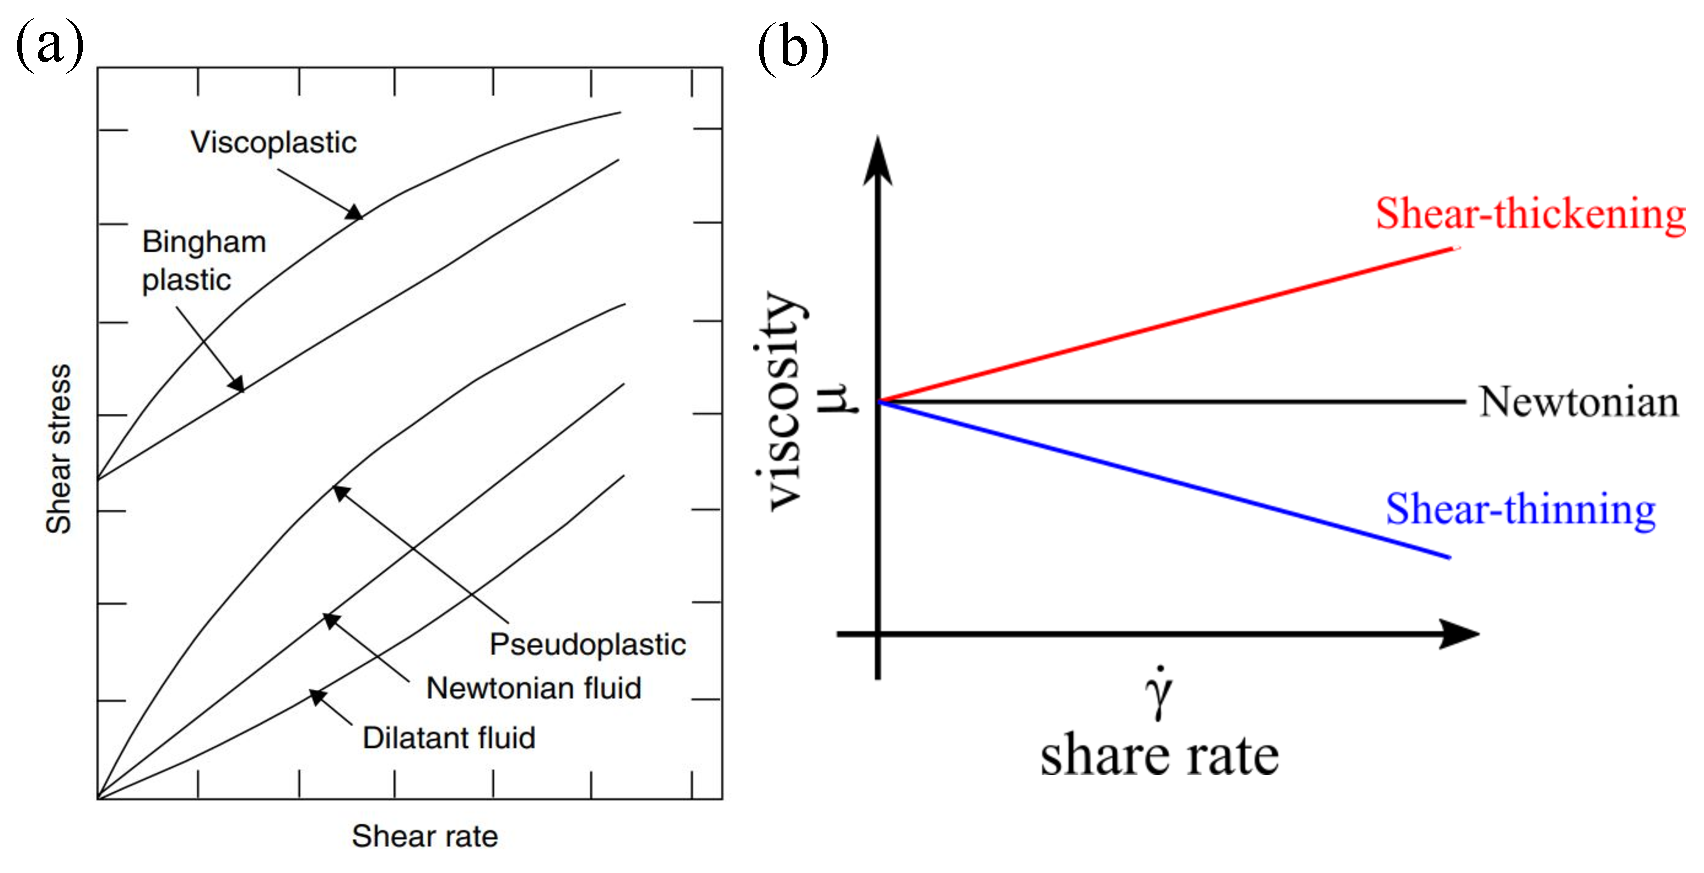
\includegraphics[width=1\textwidth]{1-Background/shea-thining.eps}
    \caption{(a) Qualitative flow curves for different types of non-Newtonian fluids\cite{ref:1}. (b)Classifications of non-Newtonian power-law fluid.}
    \label{fig:1-fluid-curve}
\end{figure}
\begin{figure}[ht]
    \begin{center}
        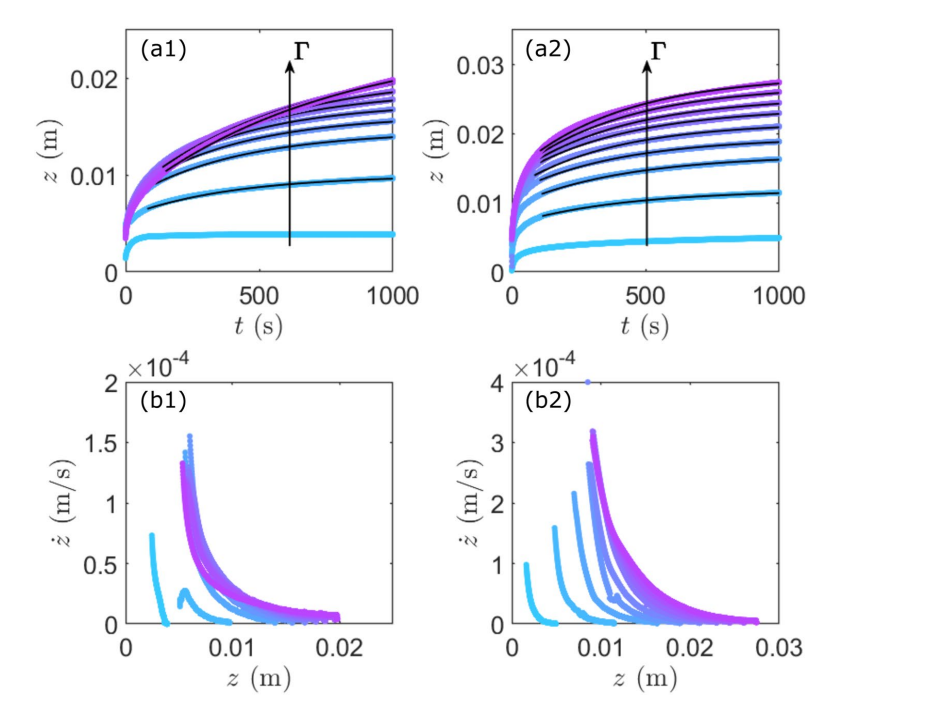
\includegraphics[width=12.0cm,clip]{1-Background/4-sinking.png}
        \caption{Sinking dynamics for different intruder-sizes and for different vibration intensities $\Gamma$. (a1) Depth$z$ versus time$t$ for $\dot{z}$ an intruder with radius of 4mm and (a2) for an intruder with radius of 7mm. (b1) Instantaneous velocity versus sinking depth $z$ obtained from (a1) and (b2) from (a2). The black lines correspond to the solutions fitted in the quasi-steady regime\cite{ref:6}.}
        \label{fig:4-sinking}
    \end{center}
\end{figure}
\newpage
\subsection{研究目的}

先行研究\cite{ref:8}において,超音波照射された擬塑性流体中を落下する球の高速化の要因として,音響境界層内部における粘度低下と,音響境界層の形成が関係していると明らかにした.また,高速化が弾性によって抑制されることを示唆していた.しかし,調査された流体や落下球の種類,径は限定的であり,弾性が高速化抑制することを明らかにしていない.

本研究で用いた試験溶液では,球の落下による運動が高速の場合,粘性による影響が支配的であり,低速の場合は弾性による影響が支配的となる.落下球の終端速度を変化させることで粘性が支配的な場合と弾性が支配的な場合に分けて,超音波照射による高速化への影響を調査した.そこで,流体物性,落下物体の密度,落下球の径をより大きく変化させ実験を行った.超音波照射された擬塑性流体中を落下する球の高速化に対する粘弾性両方の影響を明らかにすることを目的とする.

\newpage
\section{実験方法}
\label{sec:methods}
本実験では,ポリアクリルアミド(PAA)溶液(三菱ケミカル,AP805C)を擬塑性流体として用いた.初めに,試験溶液であるPAA溶液を作製し,非ニュートン流体における指標の一つとなる粘度の計測を行うことで粘度特性を計測した.また,応力と貯蔵弾性率,損失弾性率の計測を行うことで,応力に対する弾性特性を計測した.続いて,超音波振動子によって圧力場が適切に生成されているか確認した.そして,擬塑性流体中を落下する球に対する超音波照射による影響を調べるため,球落下実験を行った.

\subsection{実験系および座標系}
\label{sec:exp-system}
本研究における実験系および座標系をFig\ref{fig:system}に示す.本研究で扱う系は,水槽中において,超音波照射された擬塑性流体中を球が落下する系である.水槽液面を原点とし,球の落下方向をy軸正の方向とする.

\begin{figure}[H]
    \centering
    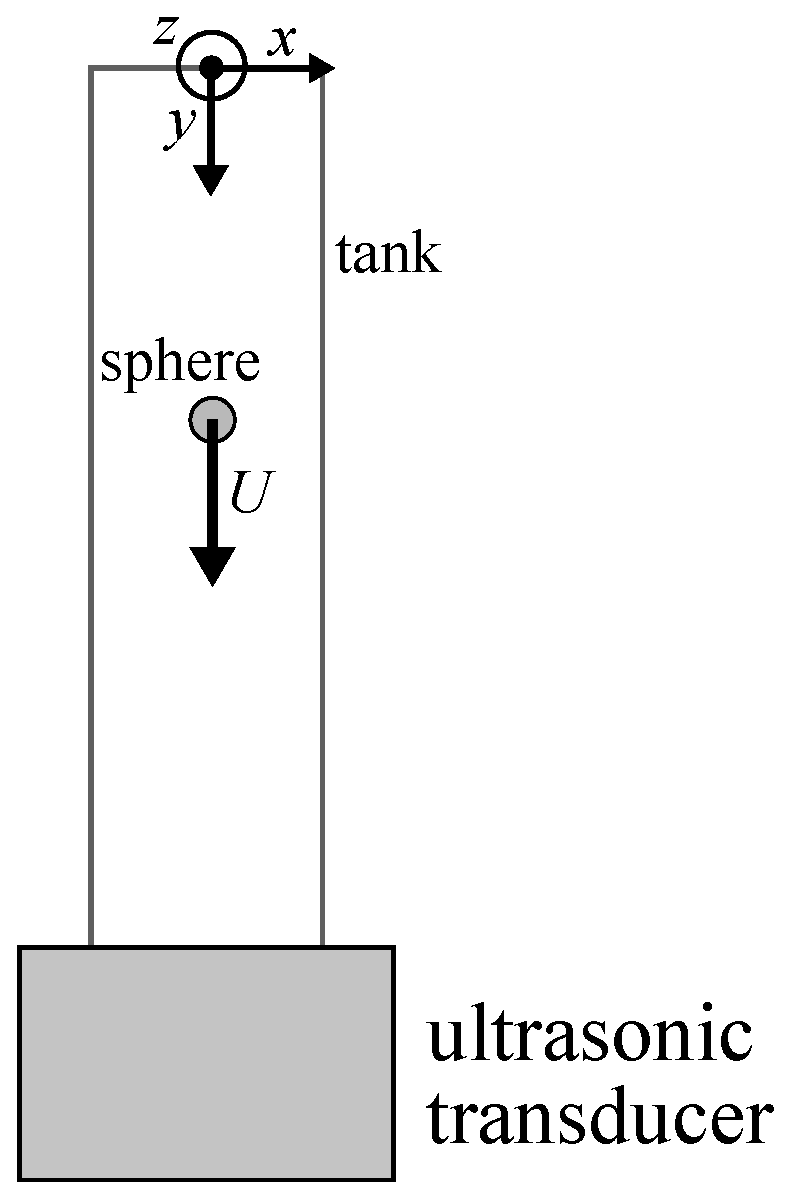
\includegraphics[width=0.32\textwidth]{./2-Methods/device-coordinate.eps}
    \caption{Experimental system and coordinate system.}
    \label{fig:system}
\end{figure}

\subsection{溶液作製}
PAA粉末と水道水を混合することで,全7種類の濃度(0.05,0.2,0.5,0.7,1.0,1.3,1.5wt.\%)のPAA溶液を作製した.以下にその作製方法を示す.

はじめに,1Lポリビーカー空容器質量をデジタルスケールを用いて計測を行った.そこに約1Lの水道水を入れ再度デジタルスケールで質量の計測を,水道水の質量の算出した.この結果より,作製する濃度に必要なPAA粉末の質量を算出し,デジタルスケールで計量を行った.このPAA粉末を水道水の攪拌を行いながら少量ずつ混合させた.これは溶液全体で均一性を持たせるためである.そして,マグネットスチーラー,プラスチック製攪拌棒を用いて溶液の攪拌を行った.これらを2回行うことで1度に約2LのPAA溶液の作製を行った.作製約1週後,溶液に気泡が見られなくなった後,ペットボトル容器に移し密封保管を行った.これは,水分の蒸発を防ぎ,濃度が大きく変化することを防ぐためである.

\subsection{粘度計測}
粘度計測における計測機器の模式図をFig\ref{fig:viscosity}に示す.ステージと回転するコーンロータの間に存在する試料によって付加されるトルクを計測することで粘度の計測を行う.粘度のせん断速度依存性を確認することで生成した溶液の性質の確認を行った.なお、計測範囲の都合上、水道水では1°34′×R24のコーンロータを,PAA溶液では0.8°×R12のコーンロータをそれぞれ用いた.コーンロータを用いることで,試料全域に同じひずみ速度を与えた.

\begin{table}[h]
    \centering
    \caption{Specifications of viscometer(東機産業,TVE-25L)}
    \label{table:viscometer}
    \begin{tabular}{c|c}\hline
        測定方式    & 円錐平板方式                    \\ \hline
        回転速度    & 0,0.1~100.0rpm;0.1rpmステップ \\ \hline
        精度/再現性 & \begin{tabular}{c}
                          フルスケールの±1.0\%以内/ \\
                          フルスケールの±0.2\%以内
                      \end{tabular}       \\ \hline
    \end{tabular}
\end{table}
\begin{center}
    \begin{figure}[H]
        \centering
        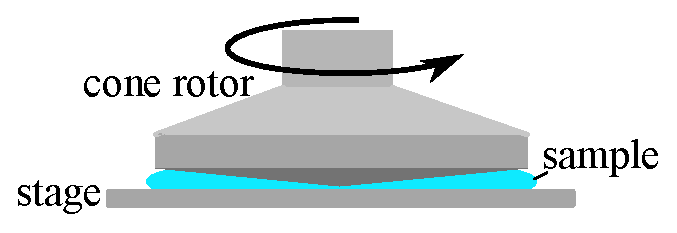
\includegraphics[width=0.5\textwidth]{2-Methods/Viscosity-Measurement.eps}
        \caption{Viscosity measurement method.}
        \label{fig:viscosity}
    \end{figure}
\end{center}

\subsection{粘弾性計測}
作製したPAA溶液の粘弾性特性を調べるため,貯蔵弾性率$G'$と損失弾性率$G''$の応力依存性を計測した.以下に,その計測理論と計測手法を示す.

\subsubsection{計測理論}
周期的なひずみを試験溶液に印可し,そのときの応力を計測することで貯蔵弾性率$G'$と損失弾性率$G''$の計測を行う.試験溶液にひずみが,
\begin{eqnarray}
    \gamma=\gamma_1e^{i\omega{}t} ,
\end{eqnarray}
で与えられたとする.粘弾性体では,ひずみは応力に対して位相が遅れるので,応力はひずみより位相が進む.印可されたひずみと応力の関係をFig\ref{fig:elastcity}に示す.位相差を$\eta$とすると,
\begin{eqnarray}
    \tau=\tau_1e^{i\left(\omega{}t+\eta\right)} ,
    \label{eq:tau_gamma}
\end{eqnarray}
となる.ここで,
\begin{eqnarray}
    |G| &=& \frac{\tau_1}{\gamma_1} ,
\end{eqnarray}
とおくと,式(\ref{eq:tau_gamma})は,
\begin{eqnarray}
    \tau=\gamma_1|G|e^{\left(\omega{}t+\eta\right)}=|G|\gamma{}e^{i\eta} ,
    \label{eq:tau_G}
\end{eqnarray}
と表される.ここで,
\begin{eqnarray}
    G^* &=& \frac{\tau}{\gamma}\\
    G' &=& |G|\cos\eta ,\label{eq:G_prime}\\
    G'' &=& |G|\sin\eta ,\label{eq:G_doubleprime}
\end{eqnarray}
とおくと,式(\ref{eq:tau_G})は,
\begin{eqnarray}
    G^* = |G|e^{i\eta} ,
    \label{eq:G_star}
\end{eqnarray}
となる.ここで,式(\ref{eq:G_prime}),(\ref{eq:G_doubleprime})より,
\begin{eqnarray}
    G^* = G'+iG'' ,
\end{eqnarray}
となる.ここで,$G^*$は複素弾性率,$G'$は貯蔵弾性率,$G''$は損失弾性率と呼ばれる\cite{生物レオロジー}\cite{化学者のためのレオロジー}.貯蔵弾性率と損失弾性率に関して,位相差$\eta$を用いて,
\begin{alignat}{3}
    G' & = 0 ,           & \quad G'' & = |G| ,         & \quad & \left(\text{at } \eta=0\right)               \label{eq:G_case1} \\
    G' & = |G|\cos\eta , & G''       & = |G|\sin\eta , &       & \left(\text{at } 0<\eta<\frac{\pi}{2}\right) \label{eq:G_case2} \\
    G' & = |G| ,         & G''       & = 0 ,           &       & \left(\text{at } \eta=\frac{\pi}{2}\right)   \label{eq:G_case3}
\end{alignat}
と場合分けできる.式(\ref{eq:G_case1})の場合は,応力とひずみの位相差が存在せず,粘性による影響がなく,弾性による影響のみが存在する.式(\ref{eq:G_case3})の場合は,応力とひずみの位相差が$\pi/2$で直交し,弾性による影響がなく,粘性による影響のみが存在する.式(\ref{eq:G_case2})の場合は,応力とひずみの位相差が$\pi/2$より小さいが存在し,弾性,粘性それぞれの影響があることを示している.以上より,損失弾性率$G'$は粘性影響を,貯蔵弾性率$G''$は弾性影響を表すことが分かる.式(\ref{eq:G_prime}),(\ref{eq:G_doubleprime})より,損失弾性率と貯蔵弾性率の比は,
\begin{eqnarray}
    \frac{G''}{G'} &=& \tan\eta ,
    \label{eq:loss_factor}
\end{eqnarray}
と書ける.ここで,$\tan\eta$は損失正接と呼ばれる\cite{生物レオロジー}\cite{化学者のためのレオロジー}.この損失正接は,
\begin{alignat}{2}
    \tan\eta & < 1, & \quad \left(\text{at } 0<\eta<\frac{\pi}{4}\right)     \label{eq:tan_eta_case1}         \\
    \tan\eta & > 1, & \quad \left(\text{at } \frac{\pi}{4}<\eta<\frac{\pi}{2}\right) \label{eq:tan_eta_case2}
\end{alignat}
と,場合分けできる.式(\ref{eq:tan_eta_case1})の場合は,貯蔵弾性率よりも損失弾性率の方が大きく,粘性による影響が強い.一方で,式(\ref{eq:tan_eta_case2})の場合は,損失弾性率より貯蔵弾性率の方が大きく,弾性による影響が強い.本研究では,損失正接を用いて粘性,弾性の強さを考える.

\begin{figure}[ht]
    \centering
    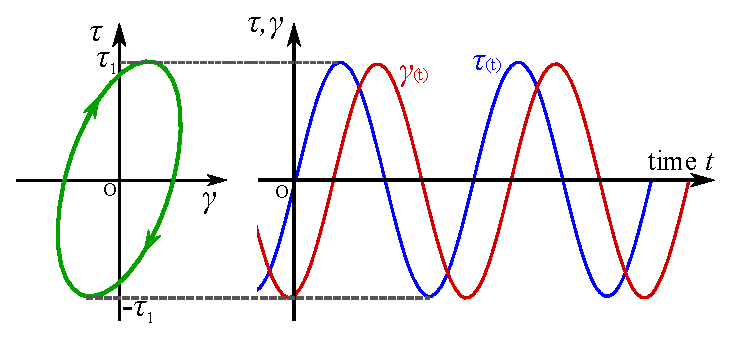
\includegraphics[width=0.75\textwidth]{2-Methods/elasticity.eps}
    \caption{Relationship between shear rate and stress in viscoelastic materials.}
    \label{fig:elastic}
\end{figure}

\newpage

\subsubsection{計測手法}

弾性率計測の概略図をFig\ref{fig:elastic-measure}に示す.計測には,回転式レオメータ(Thermo Fisher Scientific,HAAKE MARS$\rm I\hspace{-.15em}I\hspace{-.15em}I$)を用いた.回転子の振動回転周期を一定にし,振幅を変化させることで溶液に印可する応力を変化させた.回転子には1°×R30のコーンロータを用いた.計測条件をTable\ref{table:elastic}に示す.

\begin{table}[ht]
    \centering
    \caption{Elastic modulus measurement conditions.}
    \label{table:elastic}
    \begin{tabular}{c|c}\hline
        計測範囲     & $10^{-3} \sim 10^3$[Pa] \\ \hline
        計測分割数   & 70                      \\ \hline
        計測分割形式 & 対数                    \\ \hline
        計測温度     & 20[$^\circ$C](固定)   \\ \hline
        回転子周期   & 1[Hz](固定))         \\ \hline
    \end{tabular}
\end{table}

\begin{figure}[ht]
    \centering
    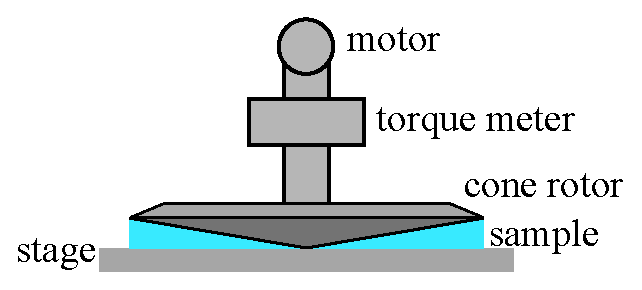
\includegraphics[width=0.7\textwidth]{2-Methods/rheometer.eps}
    \caption{Elastic modulus measurement conditions.}
    \label{fig:elastic-measure}
\end{figure}

\newpage

\subsection{圧力場計測}

圧力場計測の概略をFig\ref{fig:microphone}に示す.圧力測定にはハイドロフォン(Br\"{u}el \& Kj\ae r,Hydrophone Type8103)を用いた.ハイドロフォンの出力電圧をコンディショニングアンプ(Br\"{u}el \& Kj\ae r,NEXUS Change Amplifier Type 2692-A-0S1)を用いて増幅し,オシロスコープを用いて電圧を記録した.コンディショニングアンプの設定を元に記録した電圧を圧力場へ変換した.計測は5mm間隔で行った.この測定間隔は音速$c\approx \SI{1500}{m/s}$,周波数$f=\SI{27.4}{kHz}$としたときの波長$\lambda=c/f\approx \SI{54.7}{mm}$よりも十分に小さい.

\begin{table}[ht]
    \centering
    \caption{Specifications of microphone (Br\"{u}el \& Kj\ae r,Hydrophone Type8103)}
    \label{table:microphone}
    \begin{tabular}{c|c}\hline
        公称電圧感度 & 29$\mu$V/Pa   \\ \hline
        計測範囲     & 0.1kHz-180kHz \\ \hline
    \end{tabular}
\end{table}

\begin{table}[ht]
    \centering
    \caption{Specifications of conditioning amplifier(Br\"{u}el \& Kj\ae r,NEXUS Change Amplifier Type 2692-A-0S1)}
    \label{table:conditioning amplifier}
    \begin{tabular}{c|c}\hline
        マイクロフォン入力 &                                   \\ \hline
        入力インピーダンス & 10M$\Omega$\textbar \textbar300pF \\ \hline
        最大入力           & 31.6V                             \\ \hline
        周波数範囲(-1dB) & 0.1kHz-100kHz(ゲイン$\leq$60dB)   \\ \hline
    \end{tabular}
\end{table}

\begin{figure}[H]
    \centering
    \label{fig:microphone}
    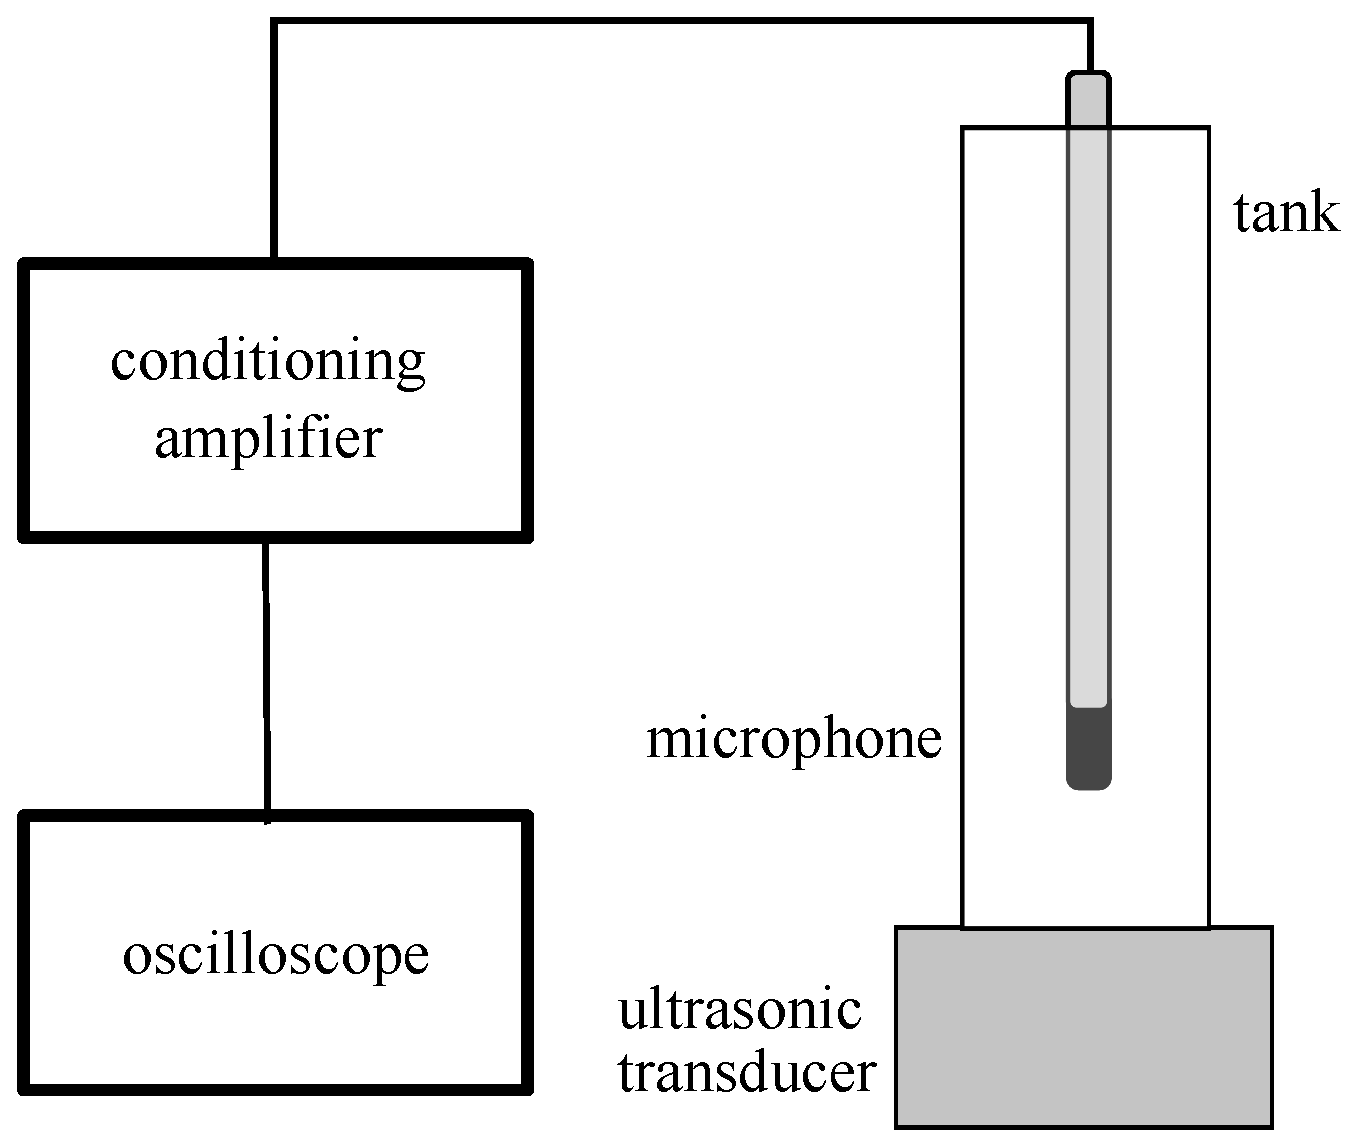
\includegraphics[width=0.7\textwidth]{2-Methods/microphone.eps}
    \caption{Schematic outline for pressure measurement.}
\end{figure}

\subsection{球落下実験}

使用した実験装置の概略図をFig\ref{fig:device}に示す.外寸にて高さ400mm,幅58mm,奥行き58mm,厚さ3mmの矩形アクリル水槽を用いた.この水槽に試験溶液を満たした.その上に,真空ポンプと接続した真空パッドを設置し,直径$D$の球を保持した.三方弁を用いて真空パッドを大気圧にすることで球の把持を解除し,球を落下させた.密度,濃度変化の場合における落下球,溶液の条件をTable.\ref{table:exp-conditions}に示す.また,球径,溶液の濃度の条件をTable.\ref{table:exp-conditions-dia}に示す.落下させた球が鋼球の場合は,ネオジム磁石を用いて試行ごとに回収した.一方で,他の種類の球は回収せずに落下実験を継続した.この際,落下球の体積によって液面が上昇するので液面の高さが一定になるよう,シリンジを用いて溶液を回収した.

球が試験液体中を落下する様子をハイスピードカメラ(BASLER, acA1920-150um)で撮影し,記録用コンピュータに連続画像(bmp形式)として保存した.解像度は0.22mm/pixelであり,最小の球(直径5mm)でも直径22.7pixelの円として撮影できる.ハイスピードカメラにはレンズ(BASLER, TS5014-MP)をつけ,絞り,焦点の調整を行い,明瞭に落下球を撮影できるようにした.実験装置後方にスクリーン,赤外線ライトを設置し,装置を後方より照射することにより,落下の様子をより分かりやすくした.さらに,超音波による影響を調査するためにアクリル水槽の下に超音波振動子を設置した.

\begin{figure}[h]
    \centering
    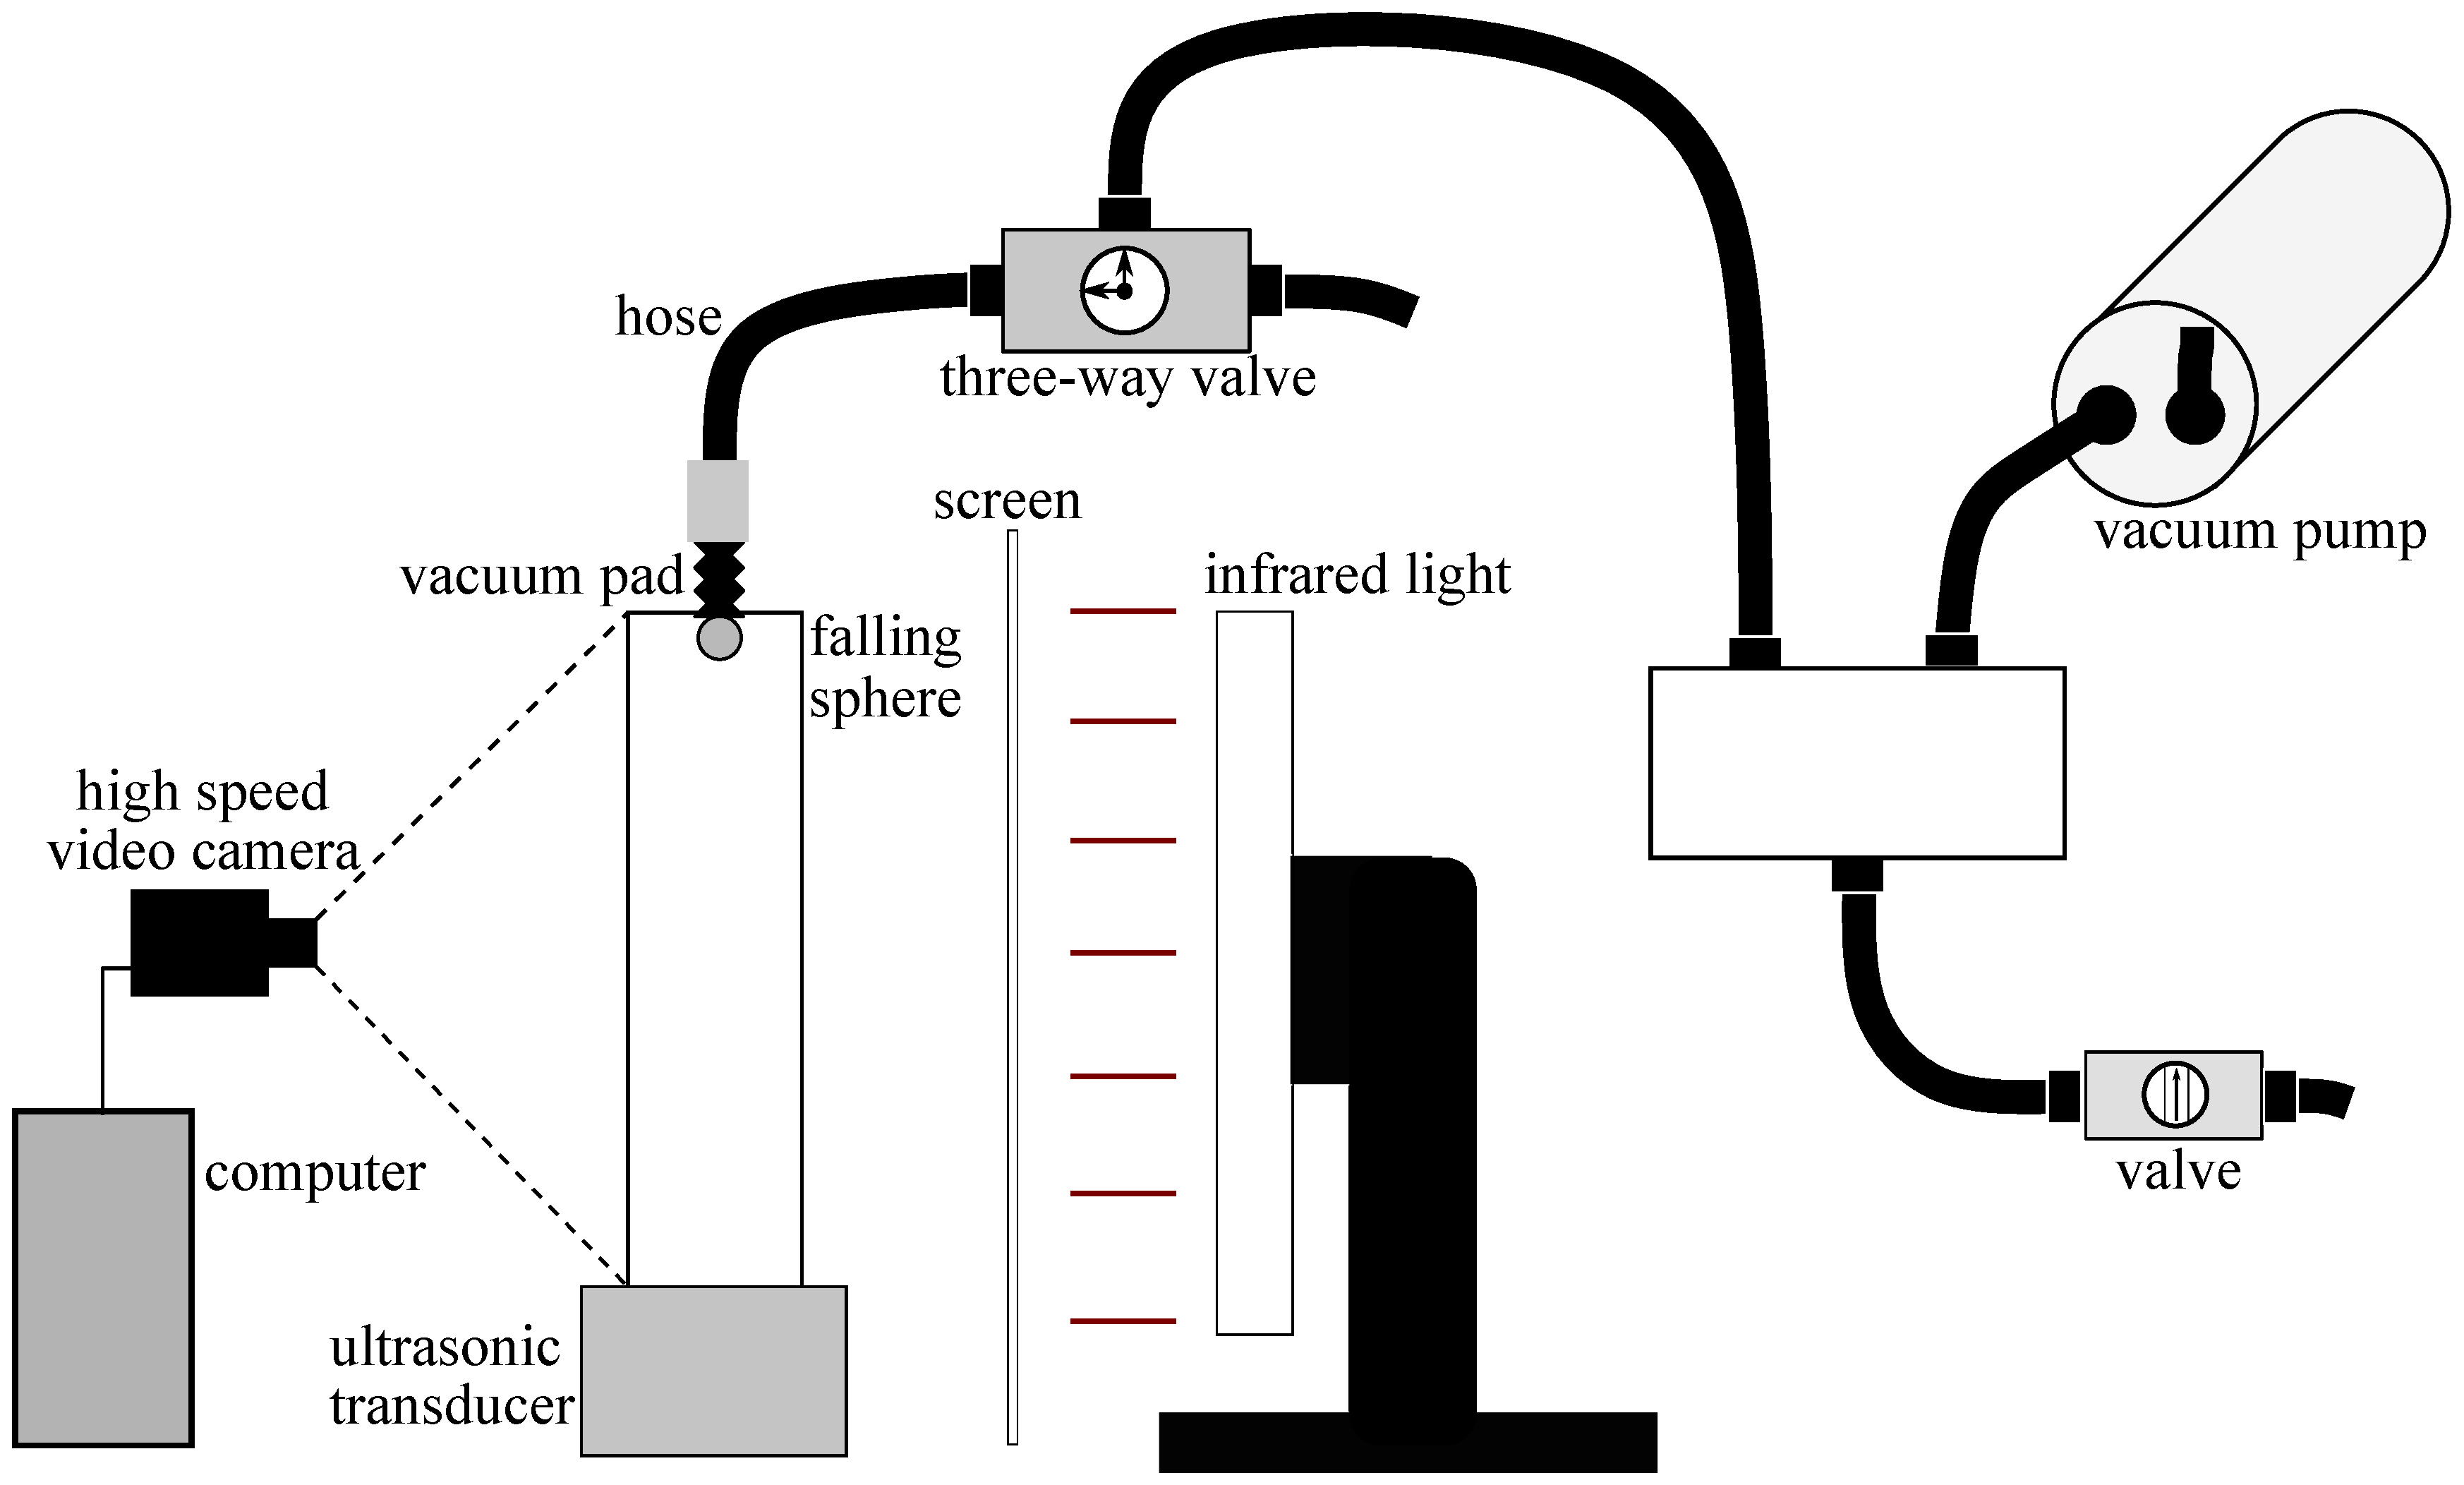
\includegraphics[width=0.9\textwidth]{2-Methods/device-vacuum.eps}
    \caption{Schematic view of the experimental apparatus.}
    \label{fig:device}
\end{figure}

\begin{table}[h]
    \centering
    \caption{Specifications of high-speed camera (BASLER, acA1920-150um)}
    \label{table:camera}
    \begin{tabular}{c|c}\hline
        センサ種別      & CMOS                      \\ \hline
        水平/垂直解像度 & 200pixel$\times$1984pixel \\ \hline
        解像度          & 0.5MP                     \\ \hline
        フレームレート  & 100fps                    \\ \hline
    \end{tabular}
\end{table}

\begin{table}[ht]
    \centering
    \caption{Specifications of lens (BASLER, TS5014-MP)}
    \label{table:lens}
    \begin{tabular}{c|c}\hline
        焦点距離[mm]     & 50.0     \\ \hline
        F値              & 1.4-16.0 \\ \hline
        最短撮影距離[mm] & 500      \\ \hline
    \end{tabular}
\end{table}

\begin{table}[H]
    \centering
    \caption{Experimental conditions of falling sphere and solution concentration.}
    \label{table:exp-conditions}
    \begin{tabular}{c|c|c|c|c|c|c}\hline
        球材質                & nylon   & アルミニウム & アルミナ & 鋼      & ステンレス & 真鍮    \\ \hline
        密度 $\rho$[kg/m$^3$] & 1130    & 2700         & 3800     & 7900    & 7900       & 8700    \\ \hline
        直径 $D$[mm]          & 9.5     & 10           & 10       & 10      & 9.525      & 9.52    \\ \hline \hline
        PAA 0.05wt.\%         & $\circ$ &              &          &         &            &         \\ \hline
        PAA 0.2wt.\%          &         & $\circ$      & $\circ$  &         & $\circ$    & $\circ$ \\ \hline
        PAA 0.5wt.\%          &         & $\circ$      & $\circ$  &         & $\circ$    & $\circ$ \\ \hline
        PAA 0.7wt.\%          &         & $\circ$      & $\circ$  &         & $\circ$    & $\circ$ \\ \hline
        PAA 1.0wt.\%          &         & $\circ$      & $\circ$  & $\circ$ &            & $\circ$ \\ \hline
        PAA 1.3wt.\%          &         & $\circ$      & $\circ$  &         & $\circ$    & $\circ$ \\ \hline
        PAA 1.5wt.\%          &         &              & $\circ$  &         & $\circ$    & $\circ$ \\ \hline
    \end{tabular}
\end{table}

\begin{table}[H]
    \centering
    \caption{Experimental conditions on steel sphere with varying sphere diameters.}
    \label{table:exp-conditions-dia}
    \begin{tabular}{c|c|c|c|c|c|c|c|c|c}\hline
        球材質       & \multicolumn{9}{|c}{鋼 $\rho$ =7900kg/m$^3$}                                                                                 \\ \hline
        直径 $D$[mm] & 5                                            & 8       & 10      & 11      & 12      & 13      & 14      & 15      & 20      \\ \hline \hline
        PAA 0.2wt.\% & $\circ$                                      & $\circ$ & $\circ$ &         &         &         &         &         &         \\ \hline
        PAA 0.5wt.\% & $\circ$                                      &         & $\circ$ &         &         &         &         & $\circ$ & $\circ$ \\ \hline
        PAA 1.0wt.\% &                                              & $\circ$ & $\circ$ & $\circ$ & $\circ$ & $\circ$ & $\circ$ & $\circ$ & $\circ$ \\ \hline
        PAA 1.3wt.\% &                                              & $\circ$ & $\circ$ &         &         &         &         & $\circ$ & $\circ$ \\ \hline
    \end{tabular}
\end{table}

超音波振動子の発振には,ファンクションジェネレータ(NF,WF1974),オシロスコープ(IWATSU,DIGITAL OSCILLOSCOPE DS-5614A),パワーアンプ(NF,HSA4101)を用いた.これらの接続をFig\ref{fig:connect-with-signal}に示す.ファンクションジェネレータによって,周波数,電圧を制御し,超音波出力の出力元となる正弦波信号を生成した.続いて,この生成された正弦波信号をパワーアンプによって,20倍のゲインをかけ増幅した.これらの信号はオシロスコープによってモニタリングし,正常に出力されているか確認した.パワーアンプで増幅された信号を,ランジュバン型振動子(富士セラミックス,FBL28502HA)に印可し,溶液へ超音波を照射した.振動子は円形のSUS製プレートに接着したものを用いた.超音波振動子の共振周波数は28kHzである.今回の実験において,照射する超音波周波数は,溶液中において共振状態となる27.4kHzに固定した.これは,溶液中の圧力振幅を最大とするためである.

\begin{figure}[h]
    \centering
    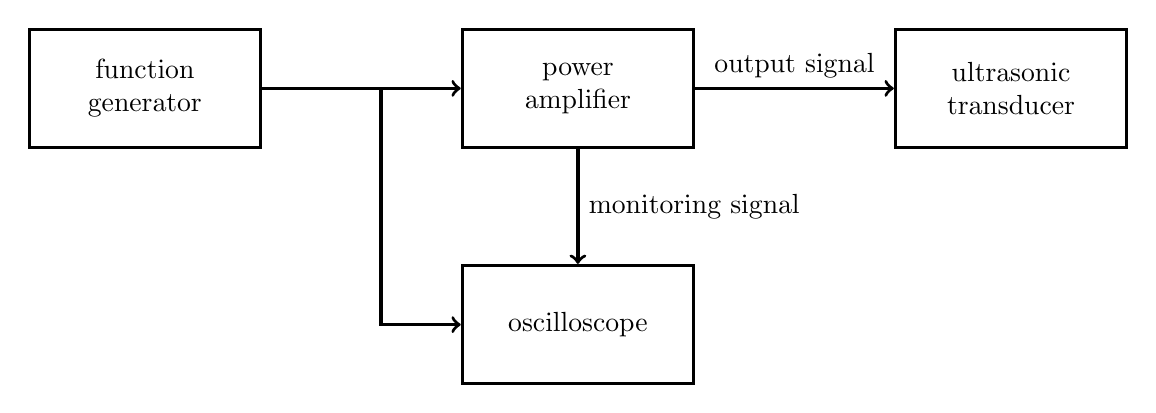
\begin{tikzpicture}[samples=100, very thick]
        \tikzset{rect/.style={rectangle,  draw,  text centered, text width=2.7cm, minimum height=1.5cm}};
        \node[rect](a) at(0,3){function \\ generator};
        \node[rect](b) at(5.5,3){power \\ amplifier};
        \node[rect](c) at(5.5,0){oscilloscope};
        \node[rect](d) at(11,3){ultrasonic \\ transducer};
        \draw[->] (a) -- (b);
        \draw[->] (3,3)--(3,0)--(c);
        \draw[->] (b) -- (c)node[pos=0.5,right]{monitoring signal};
        \draw[->] (b) --(d)node[pos=0.5,above]{output signal};
    \end{tikzpicture}
    \caption{Schematic outline for ultrasonic control system.}
    \label{fig:connect-with-signal}
\end{figure}

\newpage

\subsection{実験手順}

実験手順のフローチャートをFig\ref{fig:exp-methods}に示す.まず初めに,試験溶液であるPAA溶液を作製した.続いて,粘度を計測した.その後,圧力場を計測し,PAA溶液中に適切に圧力場が形成されているか確認した.そして,球落下実験を行い超音波照射の影響を調べた.

超音波を照射した落下実験を行う前に,球を数回落下させ,試行ごとに速度が一定となることを確認した.そして,超音波照射なしで球落下実験を行い,その後,超音波照射ありの実験を行った.超音波照射ありなしを交互に行うことによって,超音波照射による擬塑性流体中を落下する球への影響を確認した.なお,弾性を有する流体は緩和時間を代表時間として,変形した状態から元の状態へ戻ろうとする.各落下実験における流体の状態を同じとするには,十分な時間をあけて球の落下を行う必要がある.実験の再現性に関して,先行研究\cite{ref:8-5}では,等間隔の時間をあけて実験を行うと,落下速度がほぼ同じになることが報告されている.本実験においては,10分間隔で物体を落下させることで,再現性をはかった.

\begin{figure}[ht]
    \centering
    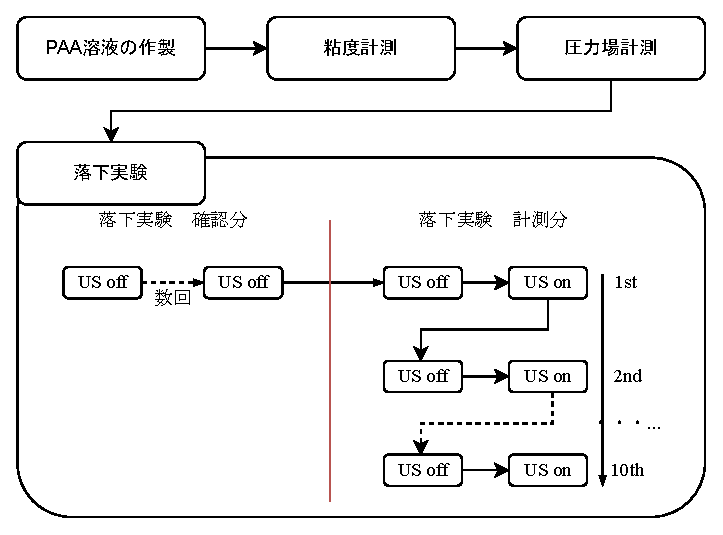
\includegraphics[width=0.7\textwidth]{2-Methods/exp-methods.eps}
    \caption{Flowchart of the experimental procedure.}
    \label{fig:exp-methods}
\end{figure}

\newpage
\subsection{解析方法}
ハイスピードカメラを用いて落下球が落下する様子をbmp形式の連続画像として撮影すると,Fig\ref{fig:expPhoto}(a) に示すように,落下球以外にも電磁石や水槽壁面が映ってしまう.この画像から,落下球を検出するためにHough変換を用いた.Hough変換は任意の幾何形状の輪郭線に対して,特徴点を一定数以上通る曲線を検出する手法である.本実験では背景処理とSobel filterを用いて,球の輪郭画像を得た.
\subsubsection{背景処理とSobel filter}
上述のように,Hough変換の前処理として,背景処理とSobel filterの処理を行った.撮影した連続画像から得た背景処理画像をFig\ref{fig:expPhoto}(b) に示す.背景処理では,画像輝度値の平均値を計算しそれぞれの画像との差分を取った.これにより,移動を伴う球抽出できる.続いて,背景処理画像にSobel filterを適用した.Sobel filter処理後の画像をFig\ref{fig:expPhoto}(c) に示す.Sobel filterとは,輪郭抽出を行うフィルタ処理である.ある任意の画素を中心とした9つの輝度値に対し,Fig\ref{fig:sobel}(a)(b)に示す係数をそれぞれ乗算し合計した後,絶対値をとる.Fig\ref{fig:sobel}(a)により$y$軸方向の輪郭を,Fig\ref{fig:sobel}(b)により$x$軸方向の輪郭を強調する.Fig\ref{fig:sobel}(a)(b)それぞれによって,フィルタ処理された9つの輝度値に対する乗算の合計値を2乗し,足し合わせた後に平方することで平均をとった.これにより,落下球の輪郭を明確にした.

\begin{figure}[h]
    \centering
    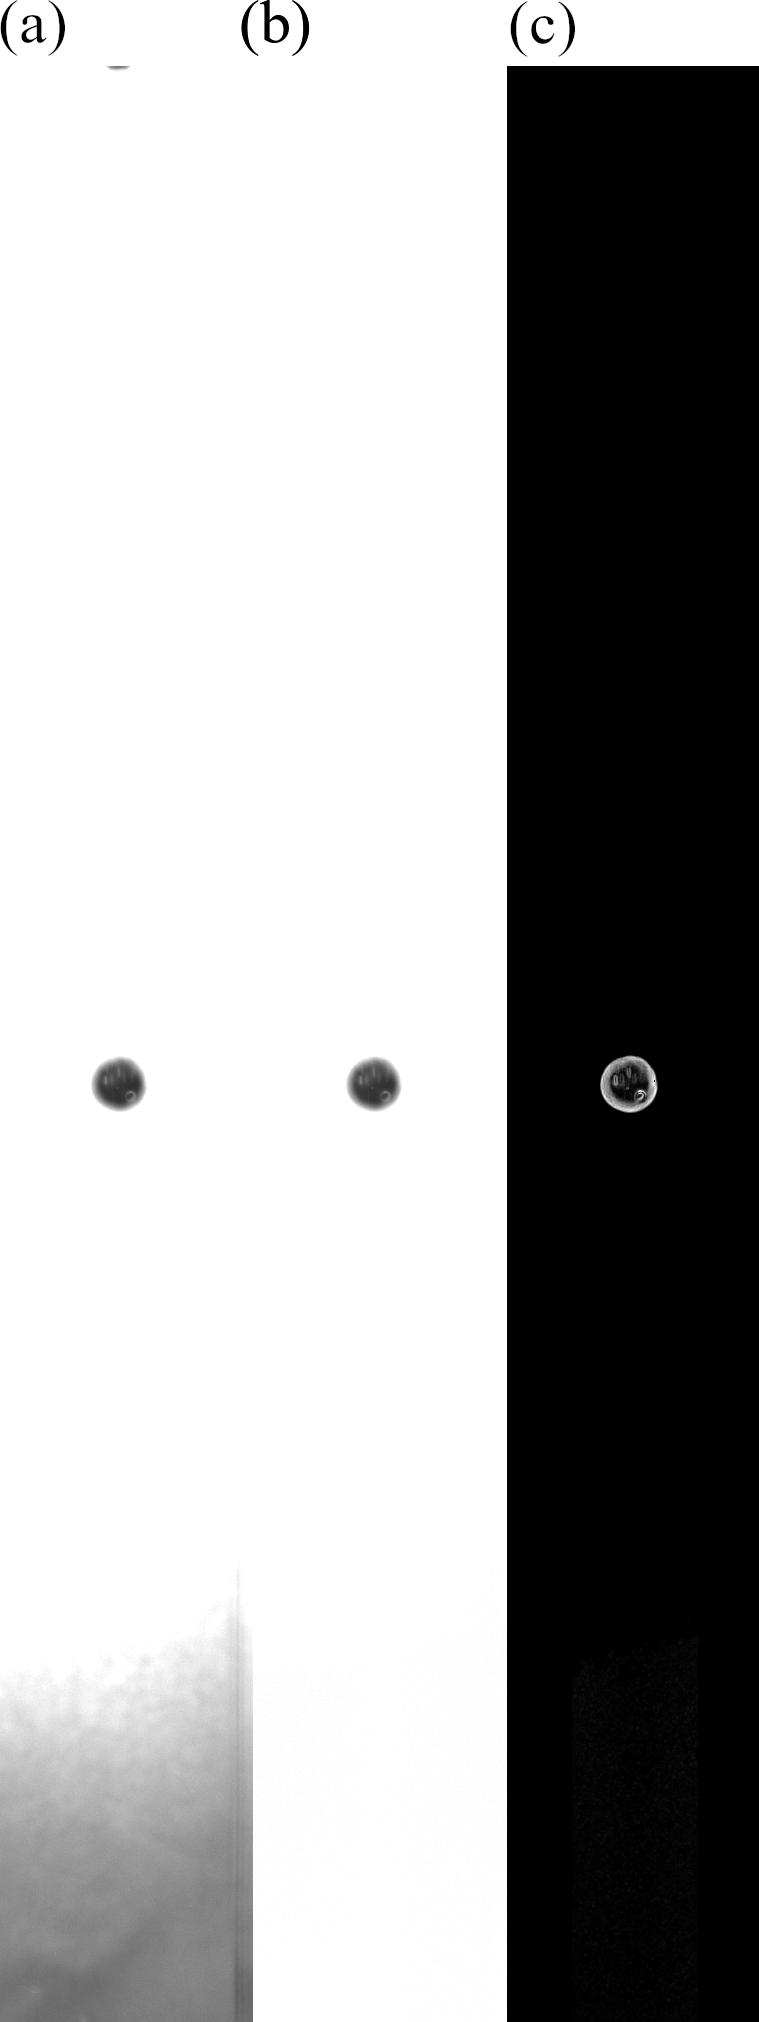
\includegraphics[width=4.0cm,clip]{2-Methods/exp-img.png}
    \caption{(a) Original image, (b) Image used by background processing and, (c) Image used by Sobel filter.}
    \label{fig:expPhoto}
\end{figure}

\begin{figure}[h]
    \centering
    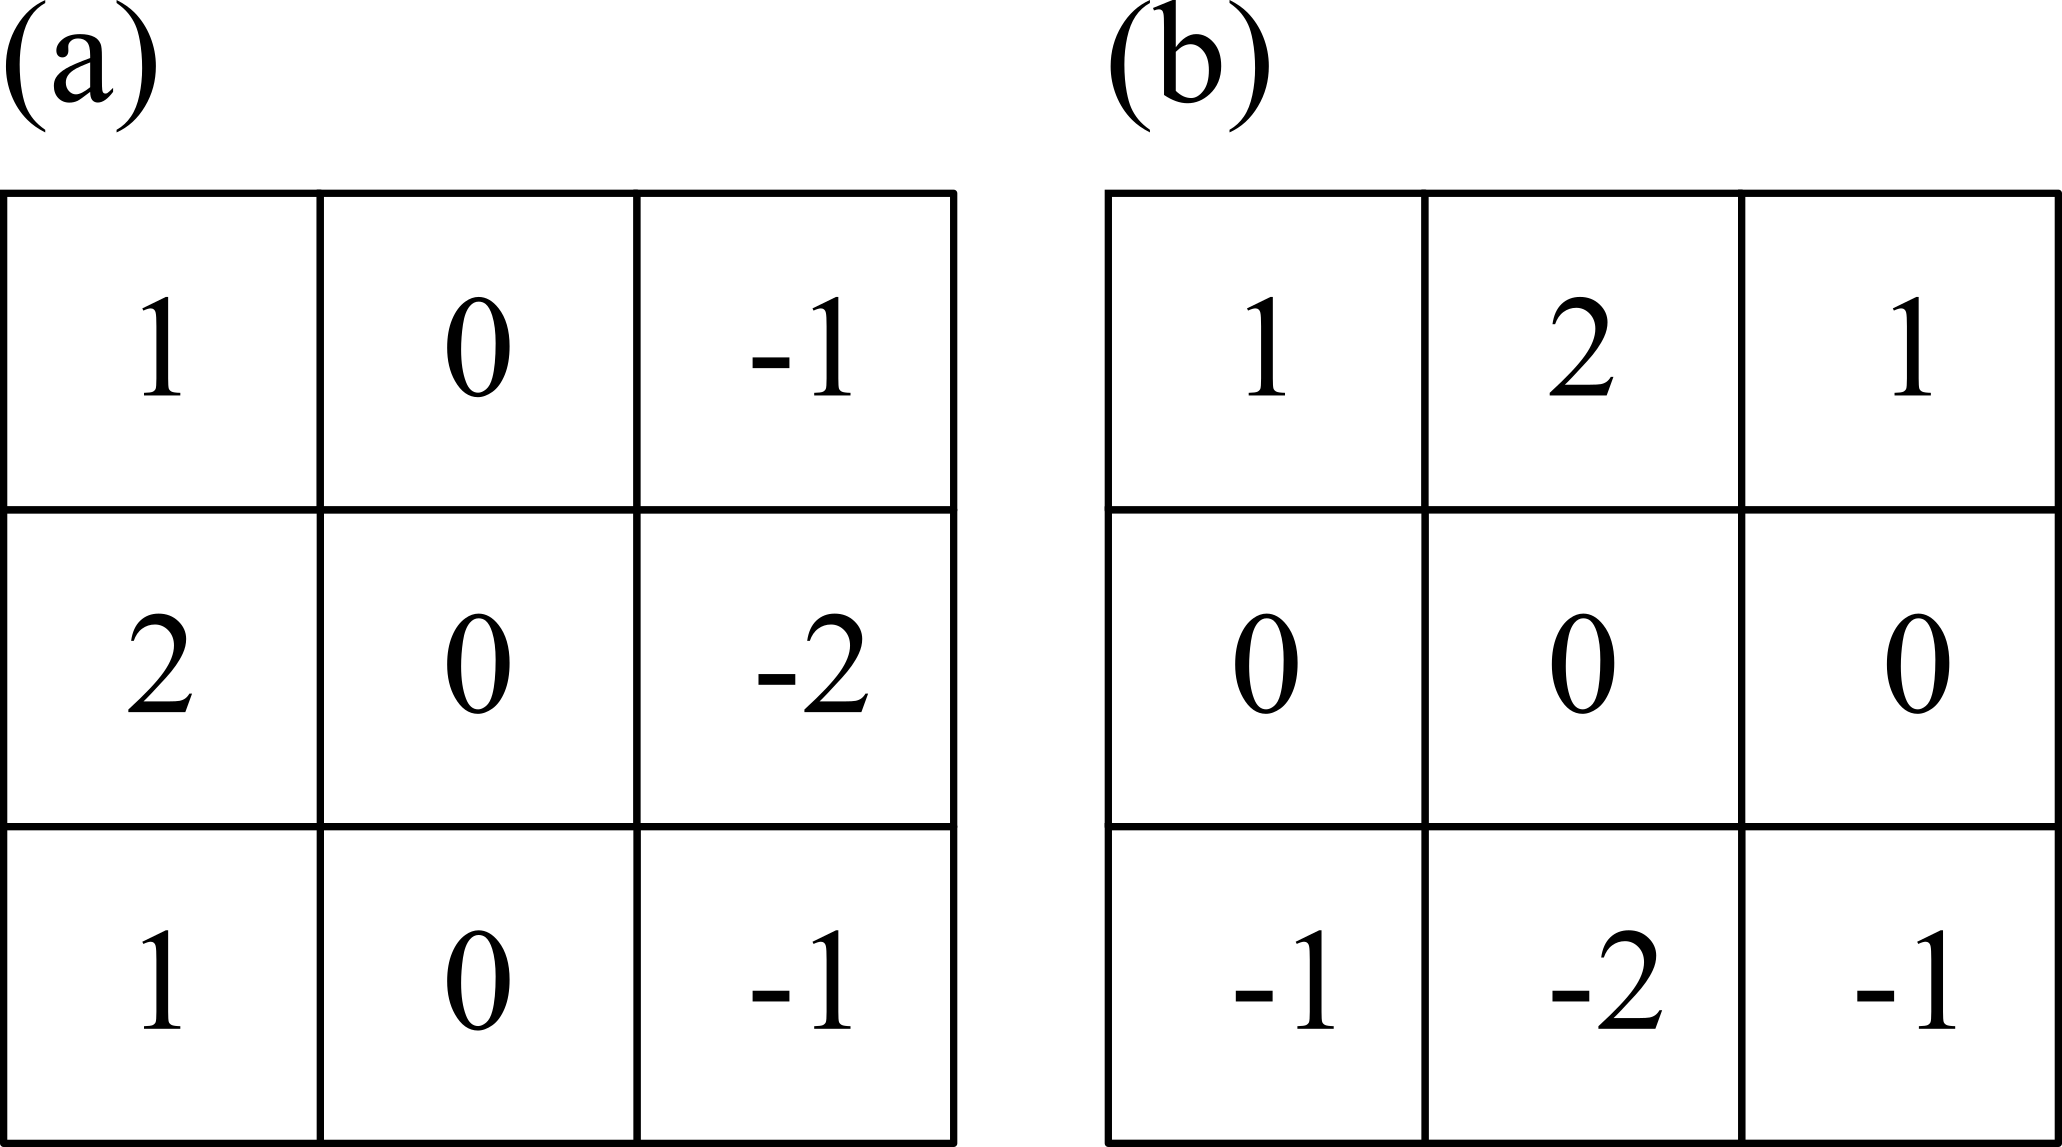
\includegraphics[width=7.0cm,clip]{2-Methods/sobel-filter.png}
    \caption{(a) Horizonal (b) Vertical Sobel filter.}
    \label{fig:sobel}
\end{figure}

\clearpage

\subsubsection{Hough変換による円の検出}
背景処理とSobel filter処理を行った画像(Fig\ref{fig:expPhoto}(c))に,Hough変換を適用し円を検出した.検出手順は,以下に示す通りである.円は中心座標と半径により一意に定まる.このことより,円の中心座標 ($x_c$, $y_c$) ,半径$r$ による1つの円$D$ ($x_c$, $y_c$, $r$) に関して考えると,Fig\ref{fig:hough}に示すように画像内における任意の座標 ($x$, $y$) を通る円は無数に存在する.3つの円の中心座標$C_1$,$C_2$,$C_3$と座標 ($x$, $y$) から円の半径$r$が計算される.無数に存在する座標 ($x, $y) を通る円の座標Dに座標 ($x$, $y$) の輝度値を加算する.この処理を画像内全ての画素に対して行う.本実験におけるHough変換では輝度値の合計が最大となる座標$D$から球の中心座標及び半径を決定した.この中心座標の時間変化より,球の落下速度を計算した.

\begin{figure}[h]
    \centering
    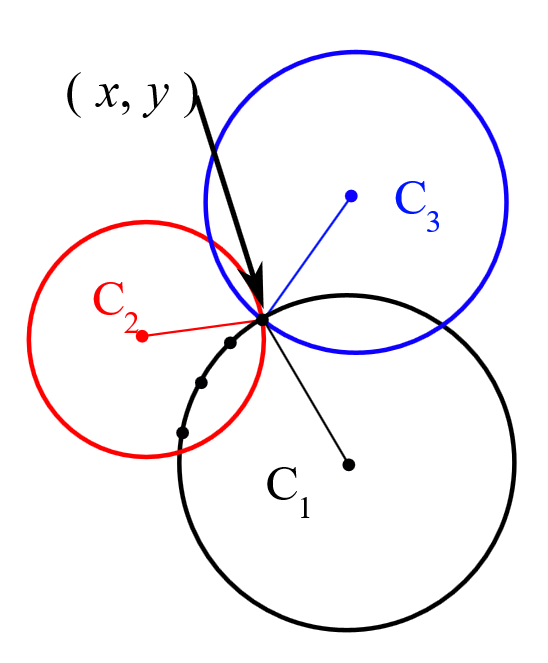
\includegraphics[width=7.0cm,clip]{2-Methods/hough.PNG}
    \caption{Outline of Hough transform.}
    \label{fig:hough}
\end{figure}

\clearpage
\section{溶液物性および圧力場の確認}
\subsection{粘度 計測結果}
球落下実験を行う試験溶液として,異なる質量濃度のPAA溶液を製作した.この製作した溶液の粘度特性を得るため,粘度計を用いて計測を行った.なお,溶媒中の溶質が不均一な状態や,混合時に混入する気泡が存在する状態では,溶液の粘度が正しく計測できない.十分な溶質拡散や脱泡のために時間を要するため,粘度計測は溶液作製直後ではなく,1週間後に行った.それぞれの試料に対し,円錐回転子の回転数を変化させることでせん断速度を変化させ,粘度を各5回計測を行いその平均を求めた.

水道水の粘度計測結果をFig.\ref{fig:vis}(a)に示す.なお,縦軸は粘度,横軸はせん断速度を表す.第2.2節においても示したが,コーンロータの回転速度に応じて,液体のせん断速度を変化させた.その結果,粘度は約1.1[mPa$\cdot$ s]でほぼ一定となっていた.これは,水がニュートン流体であり,粘度を比例係数とした速度勾配とせん断応力の比例関係となっているためであると考えられる.

水道水の場合と同様にPAA溶液の粘度計測を行った結果をFig.\ref{fig:vis}(b)に示す.なお,縦軸は粘度の対数,横軸はせん断速度の対数を表す.ここで,粘度$\mu$はせん断速度$\dot{\gamma}$に対して,粘度定数 $k$,指数$n$を用い Power-law modelに従うものとすると,
\begin{eqnarray}
	\label{eq:power-low}
	\mu=k\cdot\dot{\gamma}^{n-1}
\end{eqnarray}
といった式で与えられる\cite{ref:1}.式(\ref{eq:power-low})を用いて近似線計算を行った結果を,Table \ref{table:power-law}に示す.溶液の濃度が濃いほど,擬塑性を示す$n$は小さくなり,より擬塑性が強くなった.粘性を表す$k$は,濃度の上昇に伴い大きくなった.これらより,濃度が濃くなると,より擬塑性が強く,粘性が大きい流体となったことが分かった.

\begin{figure}[ht]
	\centering
	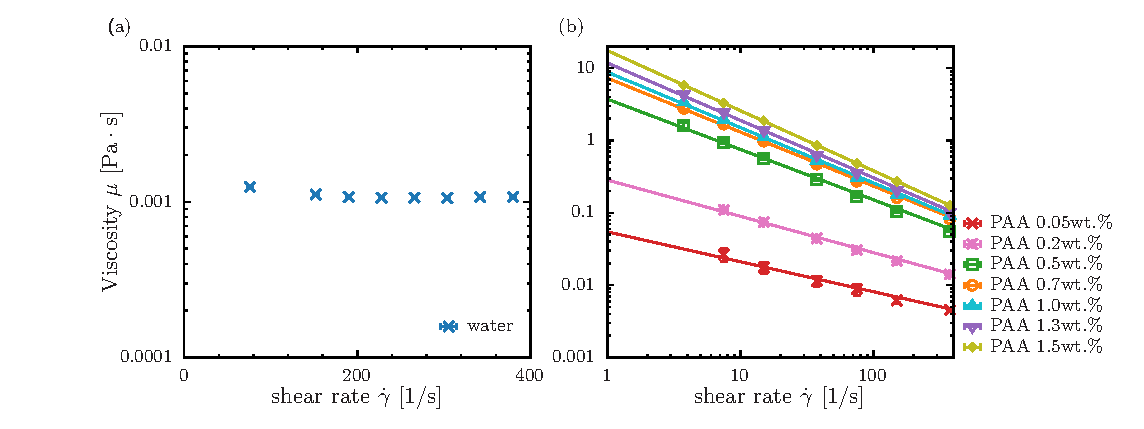
\includegraphics[width=15cm,clip]{3-Physical_Property/viscosity.eps}
	\caption{Viscosity versus shear rate for (a) tap water, (b) PAA solution.}
	\label{fig:vis}
\end{figure}

\begin{table}[h]
	\centering
	\caption{Parameters $k$ and $n$ in the Power-law model for each experimental result.}
	\label{table:power-law}
	\begin{tabular}{c|c|c|c|c|c|c|c} \hline
		PAA[wt.\%] & 0.05  & 0.2  & 0.5  & 0.7  & 1.0  & 1.3  & 1.5  \\ \hline \hline
		$k$        & 0.054 & 0.28 & 3.7  & 7.3  & 8.8  & 12   & 18   \\
		$n$        & 0.59  & 0.50 & 0.30 & 0.25 & 0.23 & 0.21 & 0.17 \\ \hline
	\end{tabular}
\end{table}

\newpage

\subsection{弾性率 計測結果}
\label{sec:elasticity}

作製したPAA溶液の応力に対する弾性特性を計測するため,貯蔵弾性率$G'$,損失弾性率$G''$の応力依存性を計測した.貯蔵弾性率は弾性項を,損失弾性率は粘性項を表す.また,損失正接$\tan\left(\eta\right)$は,
\begin{eqnarray}
	\label{eq:loss_factor}
	\tan\left(\eta\right)=\frac{G''}{G'} ,
\end{eqnarray}
といった式で求めた.損失正接は粘性項,弾性項の比となり,その応力において粘性,弾性いずれの影響を強く受けるか示す.損失正接が1より小さい応力では弾性が支配的,1より大きい応力では粘性が支配的である.

それぞれのPAA質量濃度における,応力に対する,貯蔵弾性率,損失弾性率,損失係数の計測結果をFig.\ref{fig:PAA-elast}に示す.印可する応力が小さい場合,損失正接が1より小さく弾性による影響が強かった.また,応力を大きくすると,損失正接が1より大きくなり粘性による影響が強くなった.これより,応力が小さい場合は弾性による影響が,大きい場合は粘性による影響が大きくなることが分かった.加えて,濃度が濃くなると,貯蔵弾性率,損失弾性率共に大きくなった.これより濃度が濃くなると溶液の粘弾性が強くなることが分かった.
また,損失正接が1となる応力$\tau$を$\tau_0$とする.各質量濃度における,$\tau_0$をTable.\ref{table:PAA-tau0}に示す.質量濃度が上昇すると,$\tau_0$が大きくなった.このことより,濃度が上昇すると弾性による影響が大きくなる事が分かった.

\begin{figure}[ht]
	\centering
	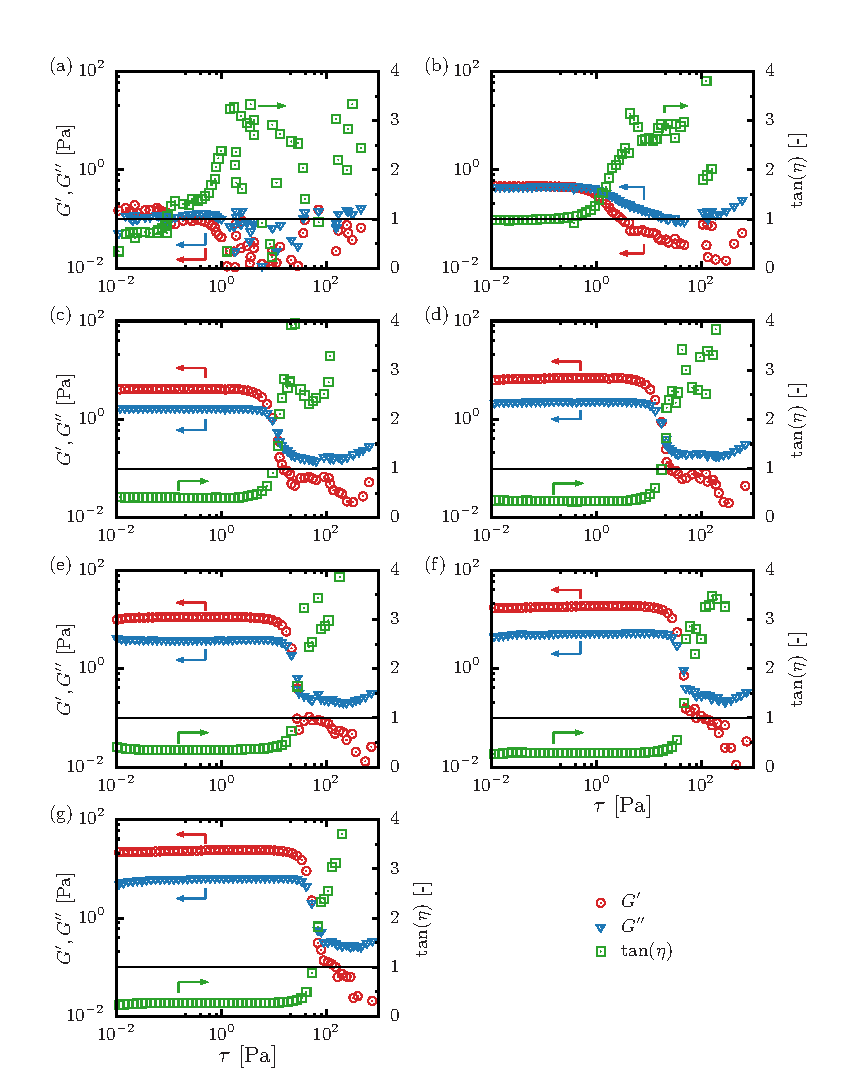
\includegraphics[width=1\textwidth]{3-Physical_Property/elastic_modulus.eps}
	\caption{Stress dependence of storage and loss elastic moduli for (a)0.05wt.\% (b)0.2wt.\% (c)0.5wt.\% (d)0.7wt.\% (e)1.0wt.\% (f)1.3wt.\% (g)1.5wt.\%.}
	\label{fig:PAA-elast}
\end{figure}

\begin{table}[h]
	\centering
	\caption{Relationship between concentration and $\tau_0$ for PAA solution.}
	\label{table:PAA-tau0}
	\begin{tabular}{c|c|c|c|c|c|c|c} \hline
		PAA[wt.\%]   & 0.05  & 0.2  & 0.5 & 0.7 & 1.0 & 1.3 & 1.5 \\ \hline \hline
		$\tau_0$[Pa] & 0.082 & 0.11 & 9.9 & 18  & 22  & 40  & 55  \\ \hline
	\end{tabular}
\end{table}

\clearpage

% //TODO:圧力振幅の溶液依存性を示す
\subsection{圧力振幅 計測結果}

それぞれの質量濃度において,超音波圧力振幅の計測を行った.超音波圧力振幅の結果をFig.\ref{fig:pressure}に示す.縦軸は水槽底面からの高さ,横軸は圧力振幅である.この結果を元にTable \ref{table:press}に,圧力振幅$\Delta{}P$の$y$方向平均値を示す.水槽全体に圧力振幅が発生していることが確認された.

% //TODO:圧力振幅の結果を入れる
\begin{table}[h]
	\centering
	\caption{Averaged value of pressure amplitude.}
	\label{table:press-A}
	\begin{tabular}{c|c|c|c|c|c|c|c} \hline
		PAA[wt.\%]             & 0.05 & 0.2 & 0.5 & 0.7 & 1.0 & 1.3 & 1.5 \\ \hline \hline
		$\bar{\Delta{}P}$[kPa] &      &     &     &     &     &     &     \\ \hline
	\end{tabular}
\end{table}

\begin{figure}[ht]
	\centering
	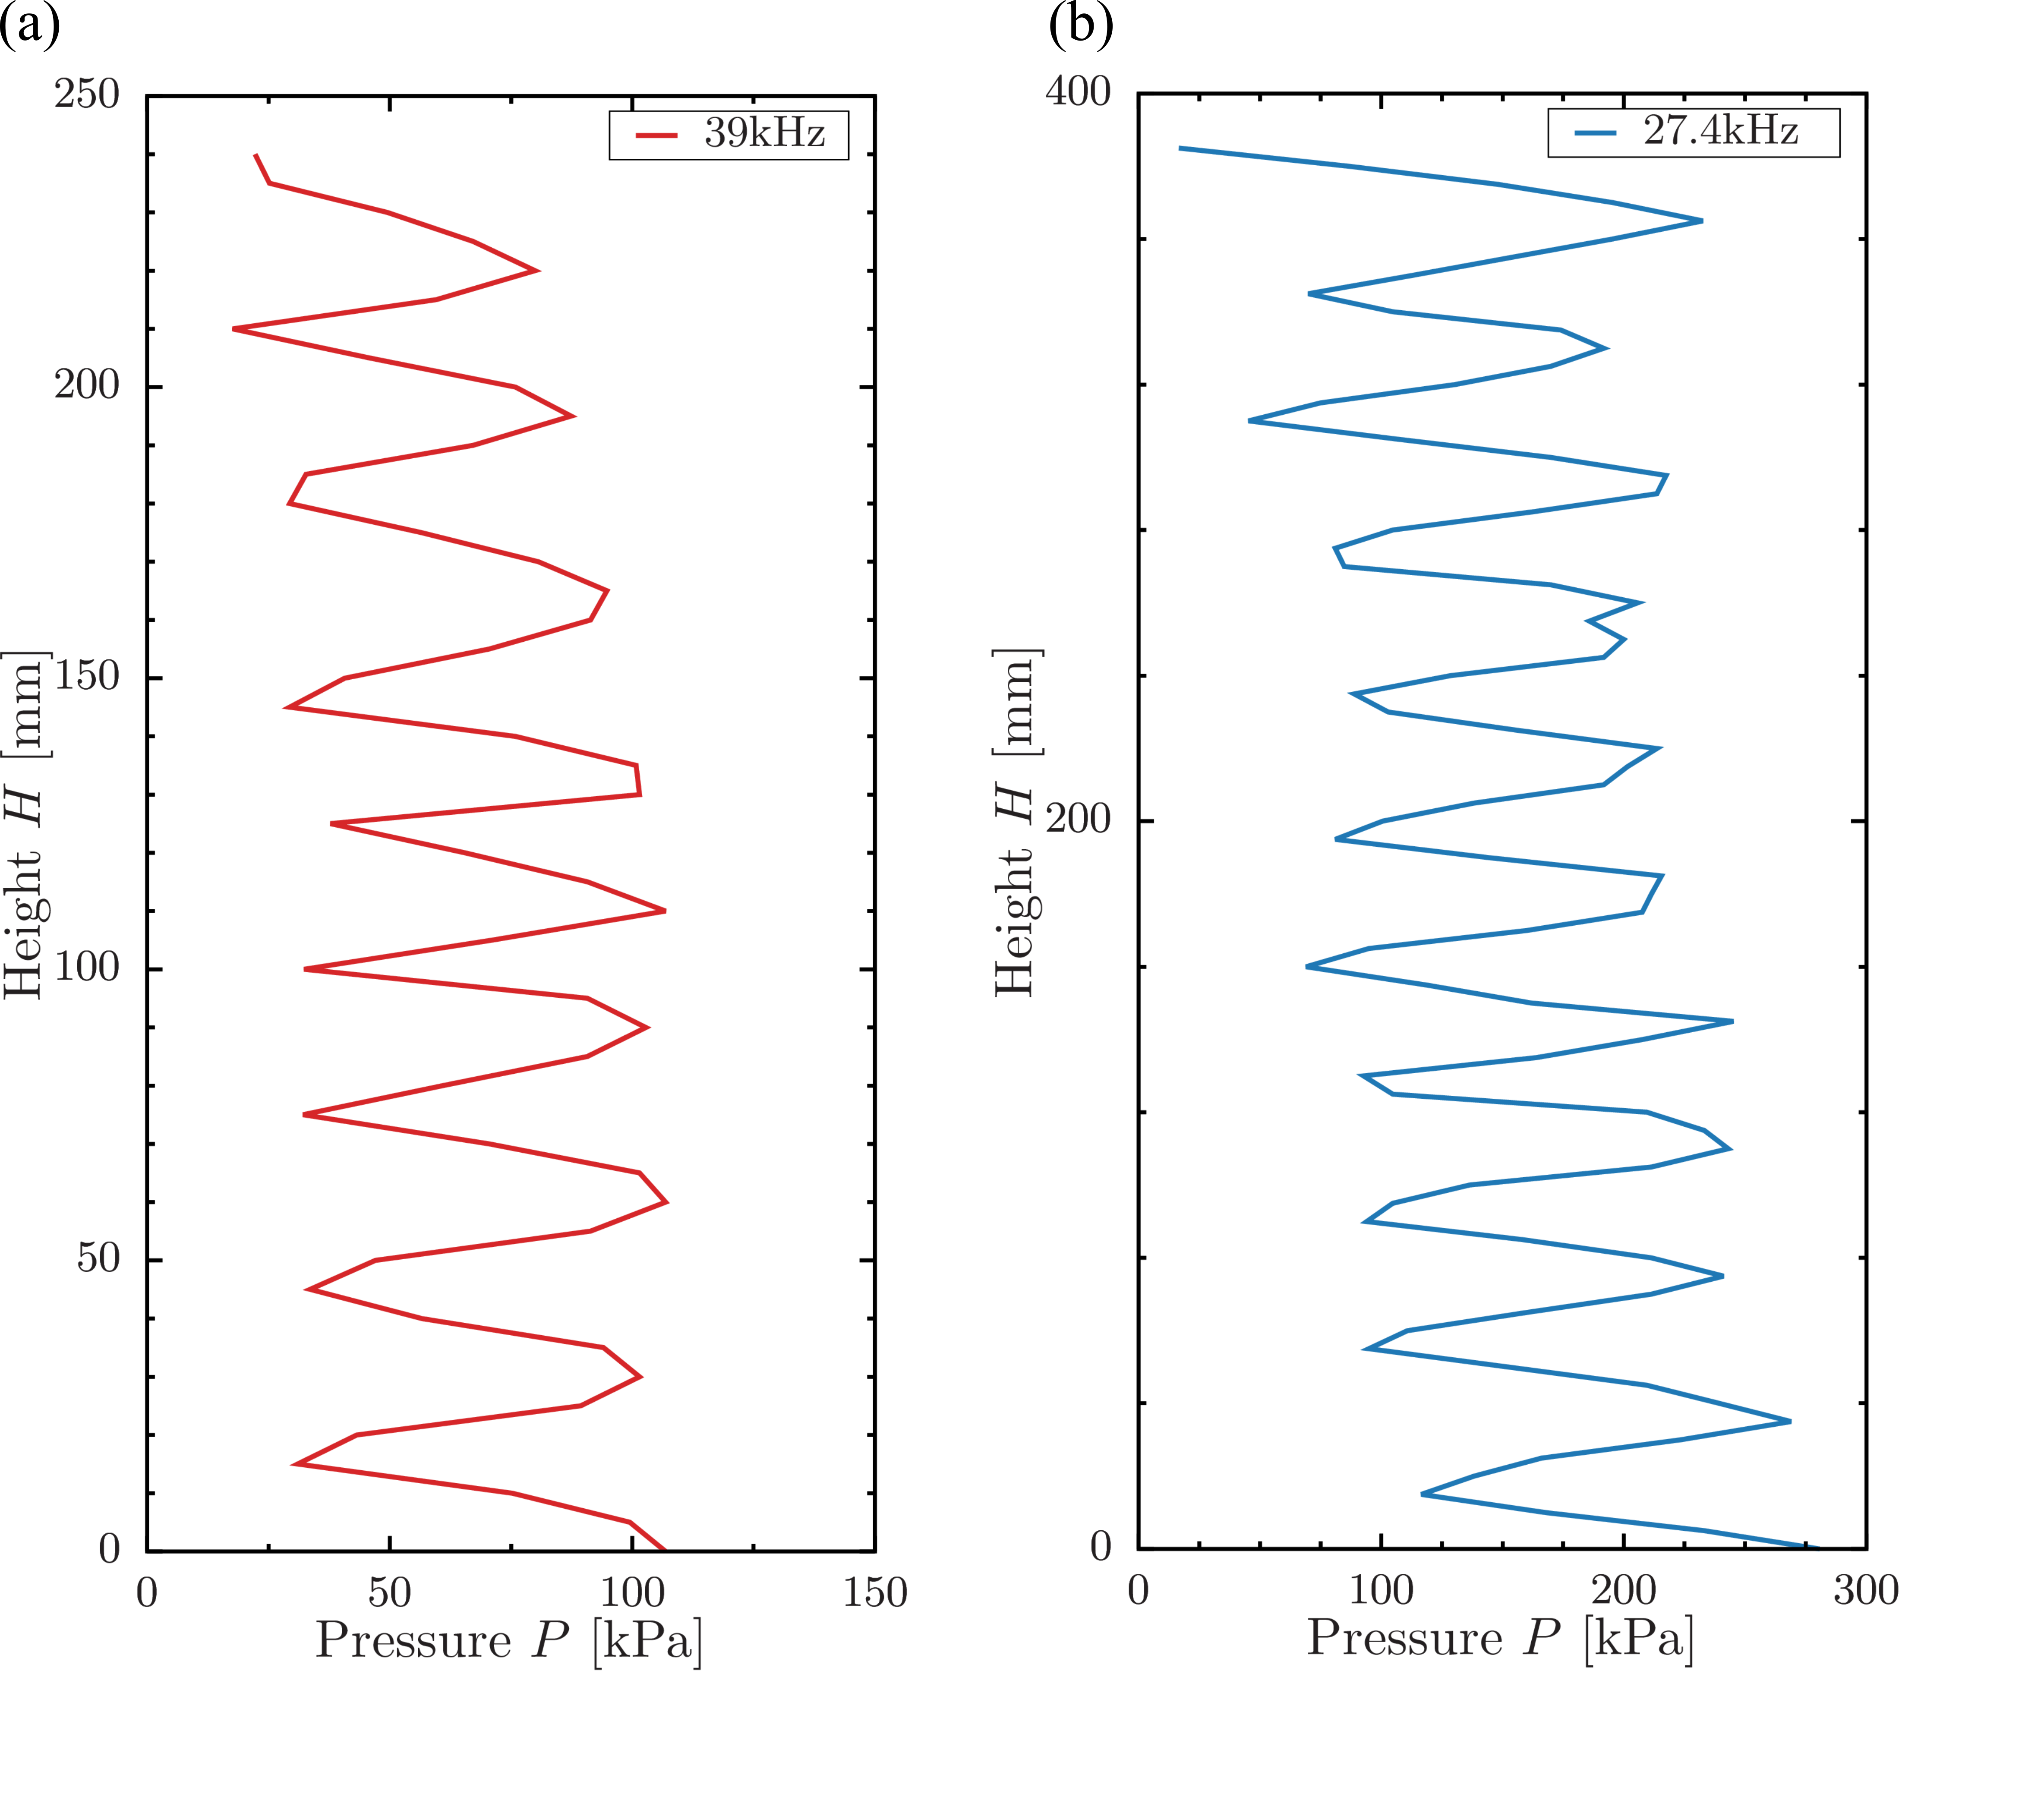
\includegraphics[width=12cm,clip]{3-Physical_Property/press.png}
	\caption{Average pressure amplitude in PAA solution.}
	\label{fig:pressure}
\end{figure}

\newpage
\section{理論}
第\ref{sec:exp-system}節で示した通り,本研究の系では超音波照射された擬塑性流体中を球が落下する.はじめに,擬塑性流体中を球が落下する理論より,球の終端速度のオーダー評価を得る.また,超音波照射による擬塑性流体中の落下球の高速化メカニズムより,落下球周囲の領域ごとの粘度のオーダー評価を得る.そして,超音波照射の有無による速度比のオーダー評価を得る.第\ref{sec:density}章以降の実験によって,これらのオーダー評価の妥当性の検証を行う.

\subsection{擬塑性流体中における球の落下}
本研究の系において,代表速度,代表長さとして,落下球の終端速度$U_\text{T}$,球直径$D=2a$を選ぶ.Power-law model (式(\ref{eq:power-low}))が適用できる流体中おける粒子レイノルズ数は次式で表される\cite{ref:1,ref:8-5}.
\begin{eqnarray}
    Re = \frac{\rho_1 \left(2a\right)^n U_T^{2-n}}{k} .
    \label{eq:re}
\end{eqnarray}
ここで,$\rho_1$は溶液密度である.今回の実験結果の代表例(鋼球,直径10mm,PAA1.0wt.\%)において,溶液密度$\rho_1\approx$1000kg/m$^3$,$2a=$0.01m,$U_T \approx$0.2m/s,$k=$8.8Pa$\cdot \text{s}^n$,$n=$0.23である.この条件を,式(\ref{eq:re})に代入すると$Re\approx$2.3と概算できる.粒子周囲の流れは慣性に比べて粘性が支配的であり,ストークス方程式に概ね従うものと考える.

超音波の伝播に関して,音波の圧力変動の時間スケールは$O\left(10^{-5}\right)$sである.これは,球の落下現象の時間スケール $O\left(10^{0}\right)$sと比べて非常に短い.球の落下に関しては,落下時間スケールで粗視化した平均的な挙動に着目する.球周囲に存在する非圧縮性流体の運動量輸送を考える.球によって誘起される応力テンソルを$\bm{\sigma}$,流体の密度を$\rho$,周囲流体の速度ベクトルを$\bm{v}$,体積力を$\bm{X}$とすると,
\begin{eqnarray}
    \rho \frac{D\bm{v}}{Dt} = \bm{X} + \nabla \cdot \bm{\sigma} ,
    \label{eq:undou}
\end{eqnarray}
となる.また,非圧縮性流体を仮定しているため,以下の連続の式が成り立つ.
\begin{eqnarray}
    \nabla \cdot \bm{v} = 0 .
    \label{eq:renzoku}
\end{eqnarray}
粒子重心位置から見た移動座標系では,式(\ref{eq:undou})の左辺は,以下のように書ける.
\begin{eqnarray}
    \frac{D\bm{v}}{Dt} = \frac{\partial \bm{v}}{\partial t} + \left(\bm{v} - \bm{U}_T \cdot \nabla \right) \bm{v} .
    \label{eq:nabie}
\end{eqnarray}
流れは十分に発達し,定常状態であると仮定すると,式(\ref{eq:nabie})の右辺第1項の時間微分項は0となる.低レイノルズ数であることからStokes近似を用いると,式(\ref{eq:nabie})の右辺第2項の慣性項は無視できる.加えて,粒子周囲流体には密度差がないため,静水圧分を除いた圧力を使って応力${\bm \sigma}$と書くと,体積力${\bm X}$は0と書ける.これらの仮定より,式(\ref{eq:undou})を以下のように簡略化する.
\begin{eqnarray}
    \nabla \cdot \bm{\sigma} = 0 .
    \label{eq:sigma-}
\end{eqnarray}

粒子重心周りの球形領域において,ガウスの発散定理を適用すると以下の関係が成り立つ.
\begin{eqnarray}
    \int_S{\bm{\sigma \cdot \bm{n}}}dS = \int_V{\nabla \cdot \bm{\sigma}}dV ,
    \label{eq:gaussian}
\end{eqnarray}
ここで,$\bm{n}$は球領域および粒子の表面での外向き単位法線ベクトル,$S$はそれぞれの球の表面積,$V$は2つの球の間の体積を表す.式(\ref{eq:sigma-})より,式(\ref{eq:gaussian})の右辺は0とする.式(\ref{eq:sigma-}),(\ref{eq:gaussian})は任意の流体体積に関して成り立つため,球の表面($r = a$)と球外部の任意の領域($r > a$)において,以下の関係が成り立つ.
\begin{eqnarray}
    \int_{r=a}\bm{\sigma}\cdot\bm{e}_r dS=\int_r\bm{\sigma}\cdot\bm{e}_r dS .
    \label{eq:inte}
\end{eqnarray}
ここで,球領域表面では$\bm{n} = \bm{e}_r$,粒子表面では$\bm{n}=-\bm{e}_r$である.式(\ref{eq:inte})は,任意の領域での,面積力の釣り合いを表す.$r = a$における時間平均応力のオーダーを$\langle\sigma\rangle_a$,$r$における時間平均応力のオーダーを$\langle\sigma\rangle_r$とそれぞれする.球の表面積は$S=4\pi r^2$であるので,式(\ref{eq:inte})より,以下の関係が成り立つとみなす.
\begin{eqnarray}
    4\pi a^2\langle\sigma\rangle_a \sim 4\pi r^2\langle\sigma\rangle_r .
    \label{eq:sigma1}
\end{eqnarray}
粒子表面での表面力と体積力の釣り合いより,以下の関係を考える.
\begin{eqnarray}
    4\pi a^2\langle\sigma\rangle_a = \frac{4}{3} \pi a^3 \Delta \rho g .
    \label{eq:sigma2}
\end{eqnarray}
となる.ここで,$\Delta \rho$は球と流体の密度差,$g$は重力加速度である.式(\ref{eq:sigma1}),(\ref{eq:sigma2})より,以下のようにオーダー評価できる.
\begin{eqnarray}
    \langle\sigma\rangle_r \sim \frac{a^3\Delta\rho g}{3r^2} .
\end{eqnarray}
低レイノルズ数で粘性項が支配的であることから,応力を以下のように概算する.
\begin{eqnarray}
    \langle\sigma\rangle_r \sim \mu \dot{\gamma} .
    \label{eq:sigma3}
\end{eqnarray}
Power-law model(式(\ref{eq:power-low}))の粘度を式(\ref{eq:sigma3})に代入して整理すると以下の関係を得る.
\begin{eqnarray}
    \dot{\gamma} \sim \left(\frac{a^3\Delta\rho g}{3r^2 k}\right)^{\frac{1}{n}} ,
    \label{eq:gamma_abs}
\end{eqnarray}
次に,エネルギー散逸に関して考える.単位時間あたりのエネルギーバランスは,位置エネルギーと粘性によるエネルギー散逸の時間変化の釣り合いとして書ける.すなわち,
釣り合うため,より,以下の式が成立する.
\begin{eqnarray}
    \int_{r>a}\bar{\epsilon}dV = 4 \pi \int^\infty_a \bar{\epsilon}r^2 dr = \frac{4}{3}\pi a^3\Delta\rho g U_T ,
    \label{eq:eg}
\end{eqnarray}
と表される.ここで,$U_T$は球の終端速度,$\bar{\epsilon}$は時間平均された単位体積当たりのエネルギー散逸率である.また,エネルギー散逸率$\bar{\epsilon}$は,以下の様に概算される.
\begin{eqnarray}
    \bar{\epsilon} \sim \langle\sigma\rangle_r\dot{\gamma} \sim \mu \dot{\gamma}^2 \sim \frac{\langle\sigma\rangle_r^2}{\mu} .
    \label{eq:eps}
\end{eqnarray}
式(\ref{eq:sigma3}),(\ref{eq:eg}),(\ref{eq:eps})より,超音波照射されていないときの終端速度$U_\text{off}$は
\begin{eqnarray}
    U_\text{off} \sim \frac{a^3\Delta\rho g}{3}\int_a^\infty\frac{dr}{\mu r^2} ,
    \label{eq:UT0}
\end{eqnarray}
と見積もられる.式(\ref{eq:power-low}),(\ref{eq:gamma_abs}),(\ref{eq:UT0})より,終端速度は下記の様に書き直される.
\begin{eqnarray}
    U_\text{off} \sim \frac{a^3\Delta\rho g}{3}  \int^{\infty}_{a} \frac{dr}{\mu r^2} \sim \left(\frac{\Delta \rho g}{3k}\right)^{\frac{1}{n}}\frac{n}{2-n}a^{\frac{n+1}{n}} .
    \label{eq:UT}
\end{eqnarray}

\subsection{超音波照射された擬塑性流体中の球周囲流体の領域に関して}
超音波照射された擬塑性流体中の球周囲流体の領域の概略図をFig\ref{fig:layer}に示す.球の周囲より音響境界層,球の落下による領域,バルク領域と分類される.音響境界層におけるせん断速度を$\dot{\gamma}_\text{ABL}$,球の落下による球周囲のせん断速度を$\dot{\gamma}_\text{U}$,バルク領域におけるせん断速度を$\dot{\gamma}_\text{Bulk}$とすると,それぞれ以下のように見積もられる.
\begin{eqnarray}
    \dot{\gamma}_\text{ABL} \sim \frac{u}{\delta} , \label{eq:dotU}\\
    \dot{\gamma}_\text{U} \sim \frac{U_\text{T}}{a} , \label{eq:UTgamma} \\
    \dot{\gamma}_\text{Bulk} \sim \frac{u}{\lambda} . \label{eq:dotB}
\end{eqnarray}
ここで,$u$は音波によって加振される流体粒子速度,$\delta$は音響境界層厚さを表す.音響境界層厚さ$\delta$は,次式のように見積もられる\cite{deshpande2001vibrational,wiklund2012acoustofluidics}.
\begin{eqnarray}
    \delta \sim \sqrt{\frac{\mu_{ABL}}{\pi \rho_h f}} ,
    \label{eq:delta2}
\end{eqnarray}
ここで,周波数$f$である.それぞれの領域のせん断速度(式(\ref{eq:dotU})-(\ref{eq:dotB}))より,Power-law model(式(\ref{eq:power-low}))を適用すると,音響境界層における粘度を$\mu_\text{ABL}$球の落下による球周囲の粘度を$\mu_\text{U}$,バルクにおける粘度を$\mu_\text{Bulk}$とすると,それぞれ以下のように見積もられる.
\begin{eqnarray}
    \mu_\text{ABL} \sim k\left(\frac{u}{\delta}\right)^{n-1} , \label{eq:muABL} \\
    \mu_\text{U} \sim k \left(\frac{U_\text{T}}{a}\right)^{n-1} ,\label{eq:muU} \\
    \mu_\text{Bulk} \sim k \left(\frac{u}{\lambda}\right)^{n-1} . \label{eq:Bulk}
\end{eqnarray}
以上より,式(\ref{eq:sigma3})を用いて球の落下による応力$\tau_\text{U}$は,以下のように見積もられる.
\begin{eqnarray}
    \tau_\text{U} \sim k \left(\frac{U_\text{T}}{a}\right)^n ,
    \label{eq:tauU}
\end{eqnarray}

\begin{figure}[ht]
    \centering
    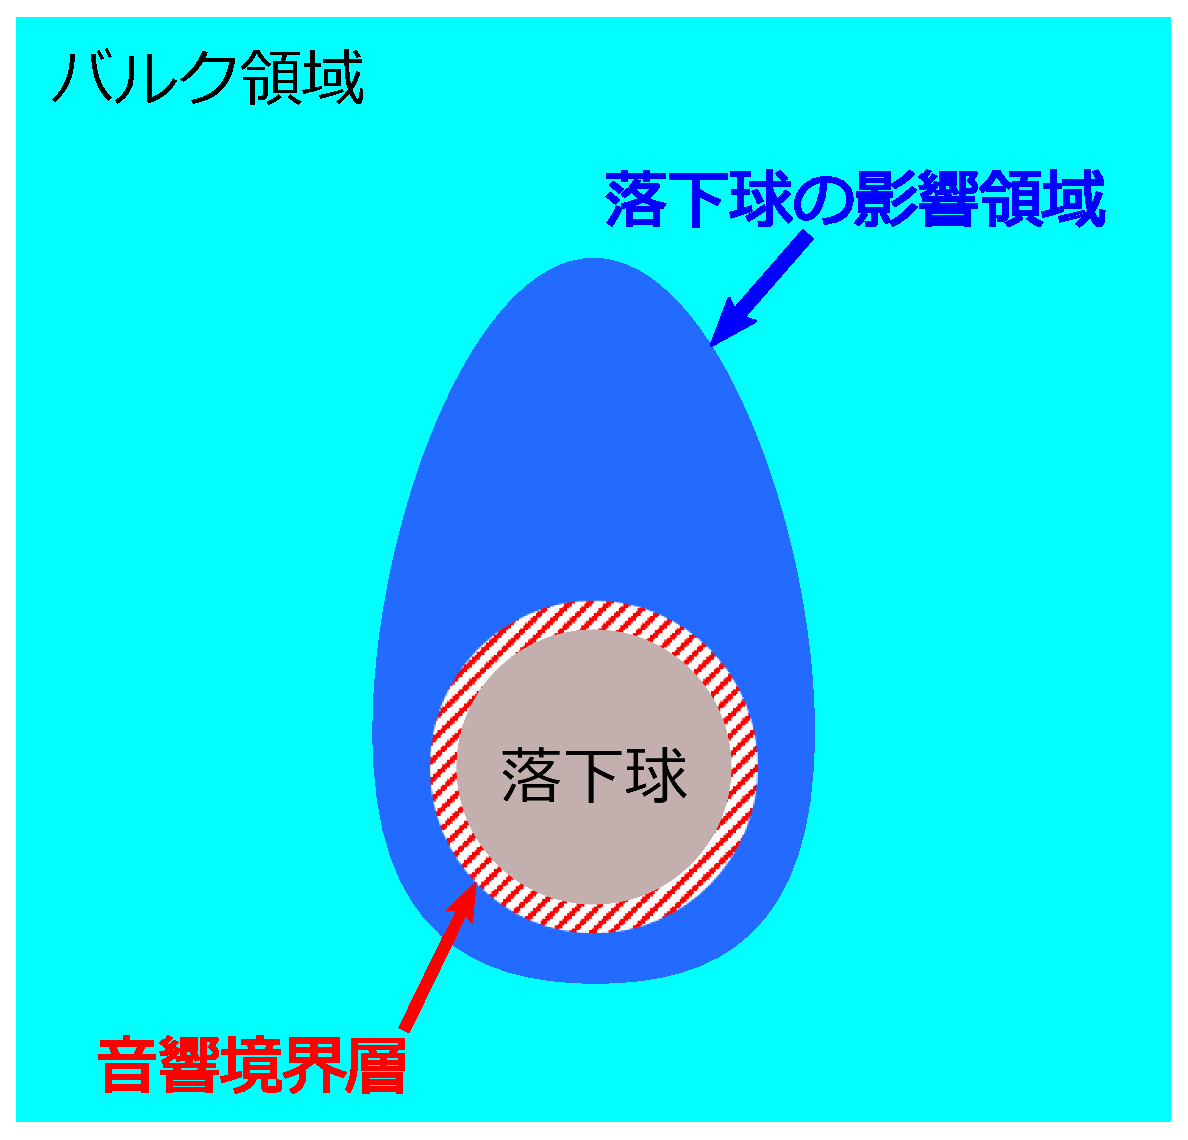
\includegraphics[width=0.5\textwidth]{4-Theory/boundary_layer.eps}
    \caption{Layers of the effect of a falling sphere on the fluid.}
    \label{fig:layer}
\end{figure}

\subsection{超音波照射に伴う球の高速化}
\label{sec:UTdiff}
流体粒子速度$u$に関して,球の落下方向を$z$とすると運動方程式は次式となる.
\begin{eqnarray}
    \frac{\partial u}{\partial t} + \frac{1}{\rho_1}\frac{\partial P}{\partial z} = 0 .
    \label{eq:newton-1}
\end{eqnarray}
ここで,$t$は時刻,$P$は圧力である.また,連続の式は圧縮性流体と仮定すると以下の式となる.
\begin{eqnarray}
    \frac{\partial u}{\partial z} + \frac{1}{\rho_1 c^2}\frac{\partial P}{\partial t} = 0 .
\end{eqnarray}
音波の周波数は一定であり,容器内の圧力変化は音波に依存するので,以下の近似を用いる.
\begin{eqnarray}
    \frac{\partial u}{\partial t} &\sim& uf ,\label{eq:1-1}\\
    \partial P &\sim& \Delta P ,\label{eq:1-2}\\
    \partial z &\sim& \lambda .\label{eq:1-3}
\end{eqnarray}
ここで,$\Delta P$は音響圧振動,$\lambda$は超音波の波長である.式(\ref{eq:1-1}),(\ref{eq:1-2}),(\ref{eq:1-3})を用いて,式(\ref{eq:newton-1})の近似を行うと次式のようになる.
\begin{eqnarray}
    uf \sim \frac{\Delta P}{\rho_1 \lambda} .
    \label{eq:u-1}
\end{eqnarray}
周波数$f$,波長$\lambda$,音速$c$の関係から式(\ref{eq:u-1})を書き換えると次式となる.
\begin{eqnarray}
    u \sim \frac{\Delta P}{\rho_1 c} .
\end{eqnarray}

音響境界層厚さ$\delta$は,式(\ref{eq:delta2})に式(\ref{eq:muABL})を代入すると,次のように表される.
\begin{eqnarray}
    \delta \sim \left(\frac{k\left(\Delta P\right)^{n-1}}{\pi \rho^n_1 c^{n-1} f}\right)^{\frac{1}{n+1}} .
    \label{eq:delta}
\end{eqnarray}

よって,超音波照射下における終端速度$U_\text{on}$は,式(\ref{eq:UT})より,
\begin{eqnarray}
    U_\text{on} \sim \frac{a^3\Delta\rho g}{3}  \int^{\infty}_{a} \frac{dr}{\mu_{ABL} r^2} \sim \frac{a\Delta \rho \delta g}{3\mu_{ABL}} ,
    \label{eq:U_ABL}
\end{eqnarray}
と見積もられる.終端速度$U_\text{off}$における,粘度$\mu_U$とする.式(\ref{eq:UT}),(\ref{eq:U_ABL})より,超音波照射の有無による終端速度比は,
\begin{eqnarray}
    \frac{U_\text{on}}{U_\text{off}} \sim \frac{\mu_U}{\mu_{ABL}}\frac{\delta}{a} ,
    \label{eq:Udiff}
\end{eqnarray}
と表される.

\newpage
\section{球密度による影響}

超音波照射された擬塑性流体中に球を落下させた結果をFig.\ref{fig:0.05-0.2}-\ref{fig:1.5}に示す.この結果より,濃度ごとに終端速度を求めた結果をFig.\ref{fig:rhoUT}に示す.縦軸は終端速度$U_\text{T}$,横軸は密度差$\Delta\rho$である.密度差が大きくなると,終端速度が大きくなることが分かった.また,濃度ごとに高速化度合を求めた結果をFig.\ref{fig:rhoUdiff}に示す.縦軸は高速化度合$U_\text{on}/U_\text{off}$,横軸は密度差である.PAA濃度0.2,1.5wt.\%においてはあまり高速化が見られなかった.一方で,0.5,1.0wt.\%において,密度差が小さくなると高速化が顕著にみられた.

超音波照射された擬塑性流体中を落下する球の高速化に対する,落下球の密度による影響を考える.\ref{sec:UTdiff}節にて示した,落下球の高速化度合の理論式(\ref{eq:Udiff})に終端速度の理論式(\ref{eq:UT})を代入すると,
\begin{eqnarray}
    \frac{U_{ABL}}{U_T} \sim \left(\frac{\Delta\rho{}g}{3}\right)^{\frac{n-1}{n}}\cdot\frac{2-n}{n}\cdot\frac{\delta}{\mu_{ABL}}\cdot\left(\frac{k}{a}\right)^{\frac{1}{n}} ,
    \label{eq:UdiffRho}
\end{eqnarray}
となる.本実験において,落下球の密度をパラメータとして考える.他の条件に関して同一であると考えると,超音波照射に伴う高速化は式(\ref{eq:UdiffRho})より,
\begin{eqnarray}
    \frac{U_{ABL}}{U_T} \sim \left(\Delta\rho{}\right)^{\frac{n-1}{n}} ,
    \label{eq:UdiffRho2}
\end{eqnarray}
と表される.

これらの結果より式(\ref{eq:UdiffRho2})を用いて,落下球と流体の密度差と,超音波照射による高速化の関係性をFig.\ref{fig:rhoUdiffAll}に示す.縦軸は高速化度合$U_\text{on}/U_\text{off}$,横軸は密度差のみによる影響を考慮した$\Delta\rho^{\left(\left(n-1\right)/n\right)}$である.全条件の結果をFig.\ref{fig:rhoUdiffAll}(a)に,0.2wt.\% PAA溶液以外の結果をFig.\ref{fig:rhoUdiffAll}(b)に示す.0.2wt\%PAA溶液の条件において,高速化度合は密度差のみによる影響に対して,相関関係は見られなかった.これは,0.2wt\%PAA溶液においてPAA濃度が非常に希薄であるため,高速化現象が発生していないためだと考えられる.一方でそれ以外の条件において,高速化度合は密度差のみによる影響に対して弱い正の相関関係を示した.これは,密度差以外の濃度による影響を考慮していないためだと考えられる.このことより,密度差を用いて超音波照射された擬塑性流体中を落下する球の高速化度合を整理することができることが分かった.

\begin{figure}[ht]
    \centering
    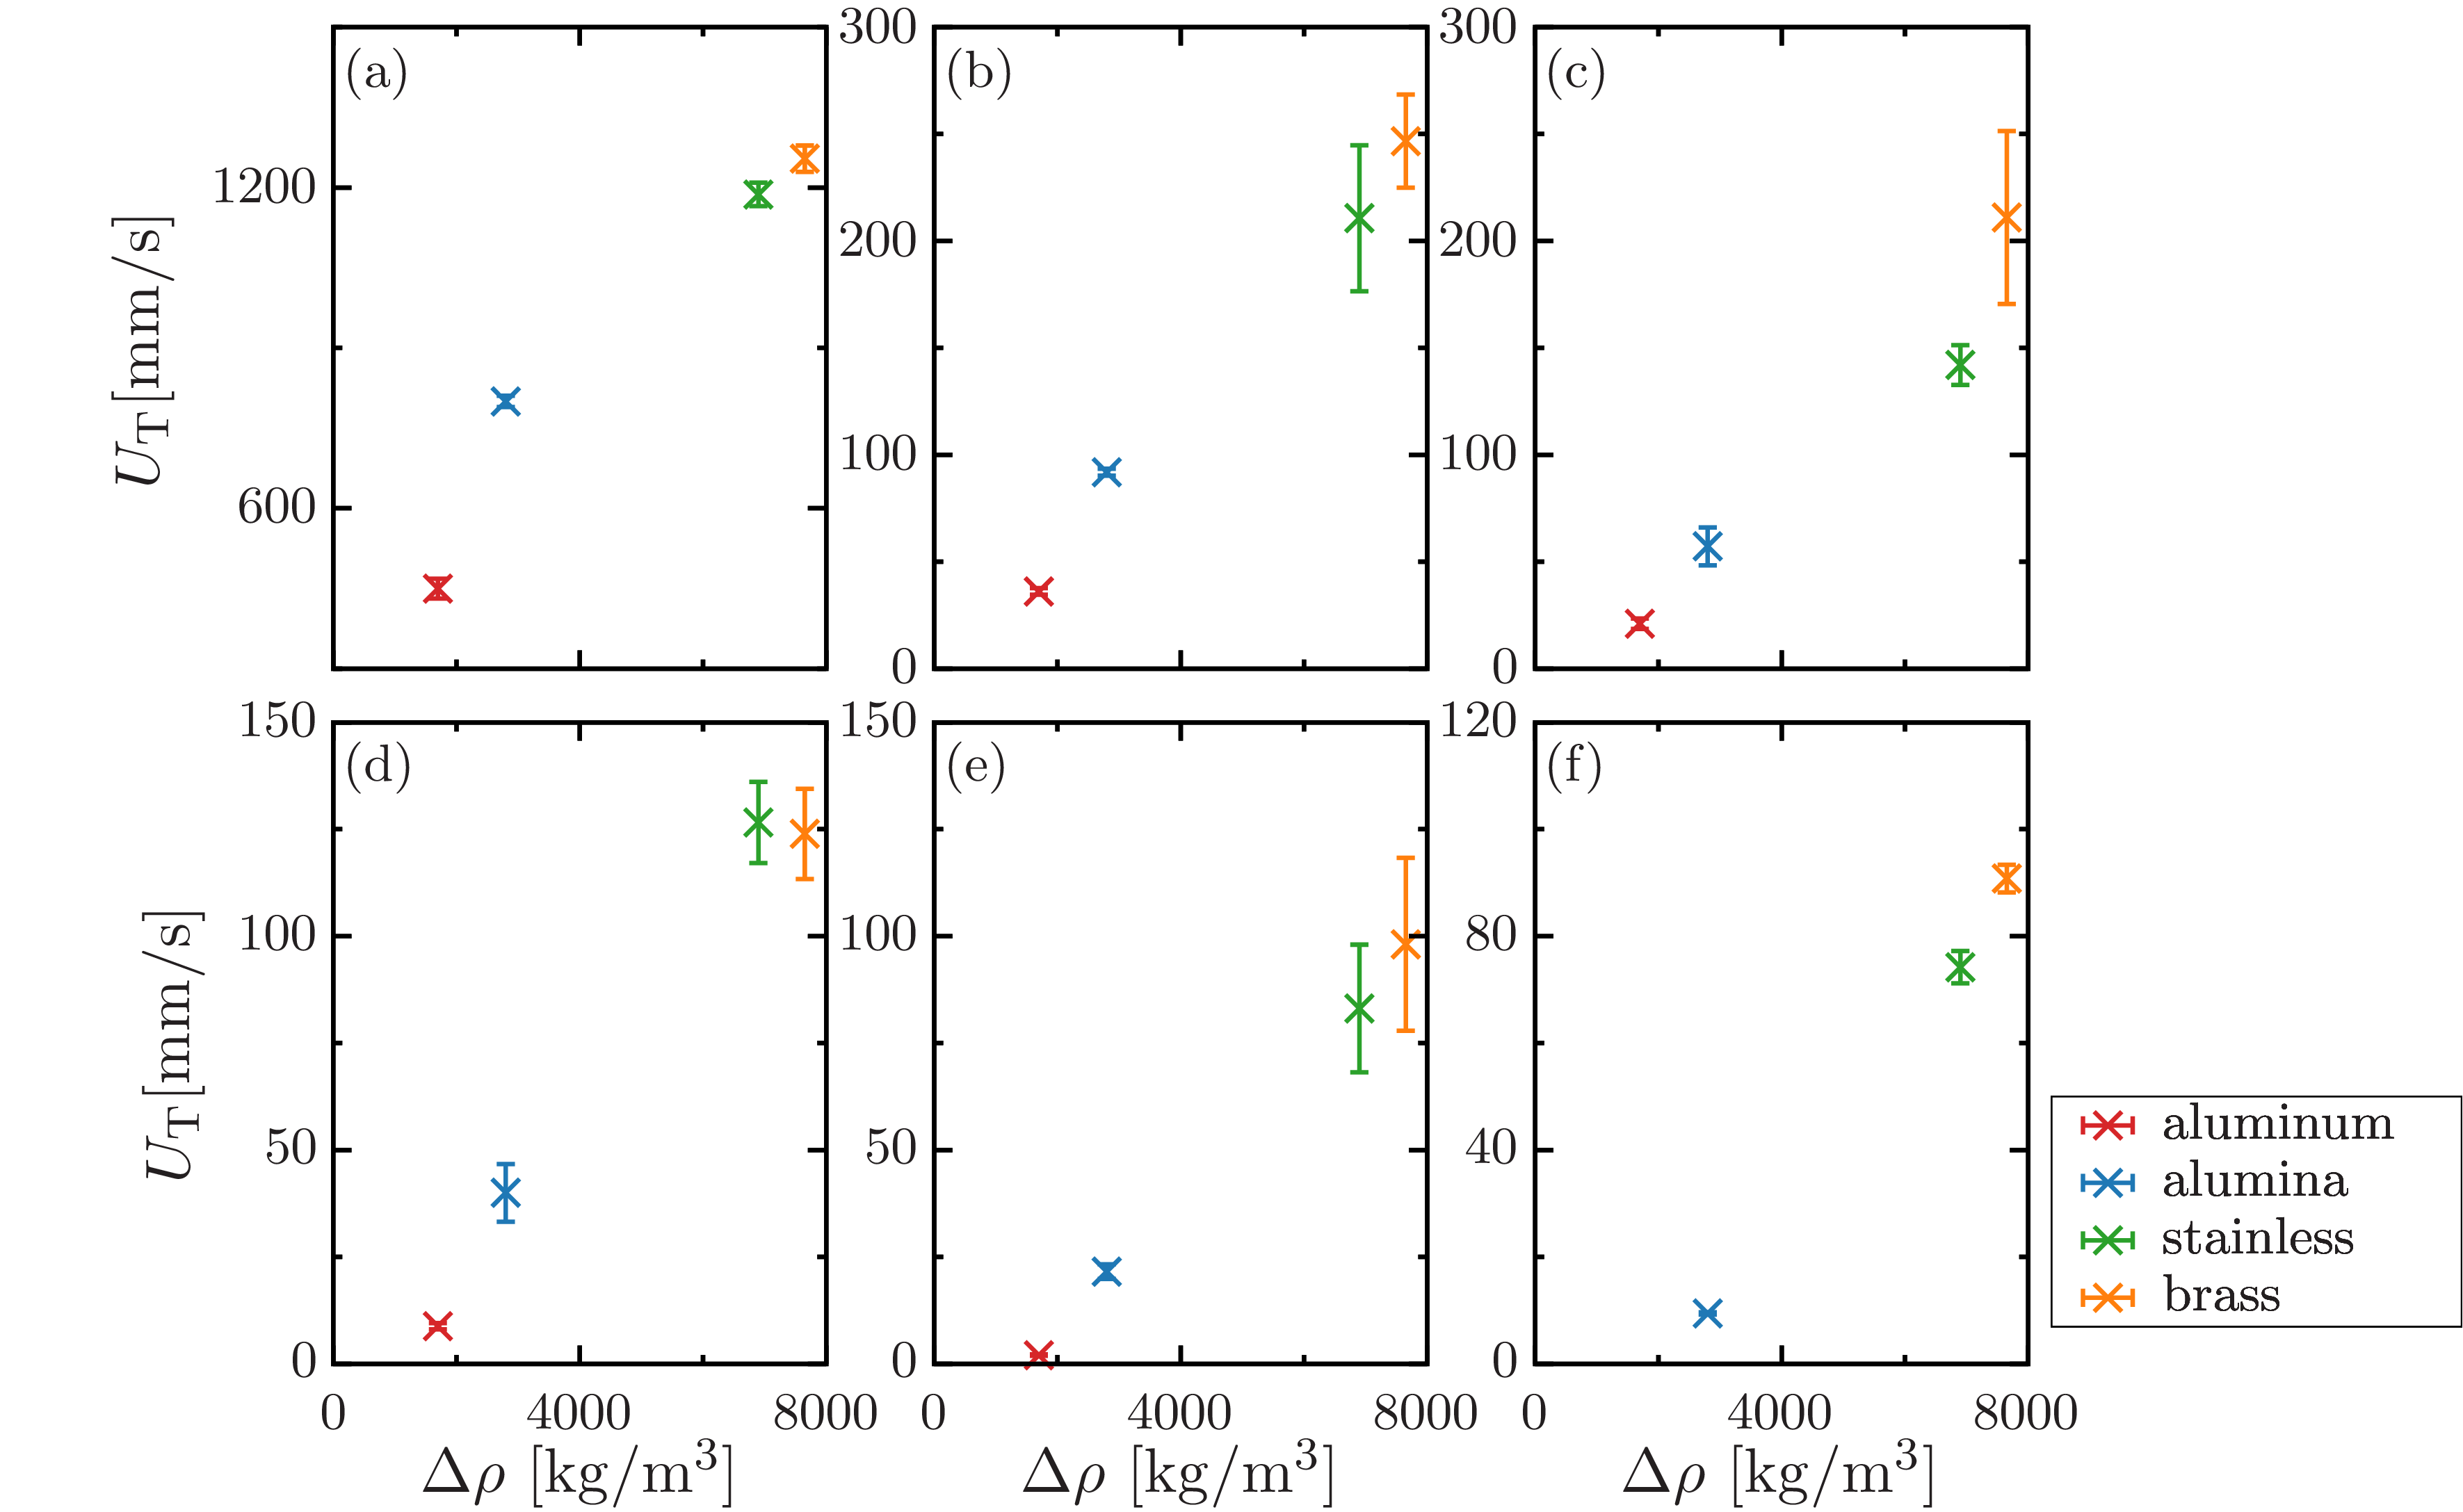
\includegraphics[width=1.0\textwidth]{./5-Results/density/rhoUT.png}
    \caption{Termination velocity by density difference in PAA solution (a)0.2wt.\%, (b)0.5wt.\%, (c)0.7wt.\%, (d)1.0wt.\%, (e)1.3wt.\%, (f)1.5wt.\%.}
    \label{fig:rhoUT}
\end{figure}

\begin{figure}[ht]
    \centering
    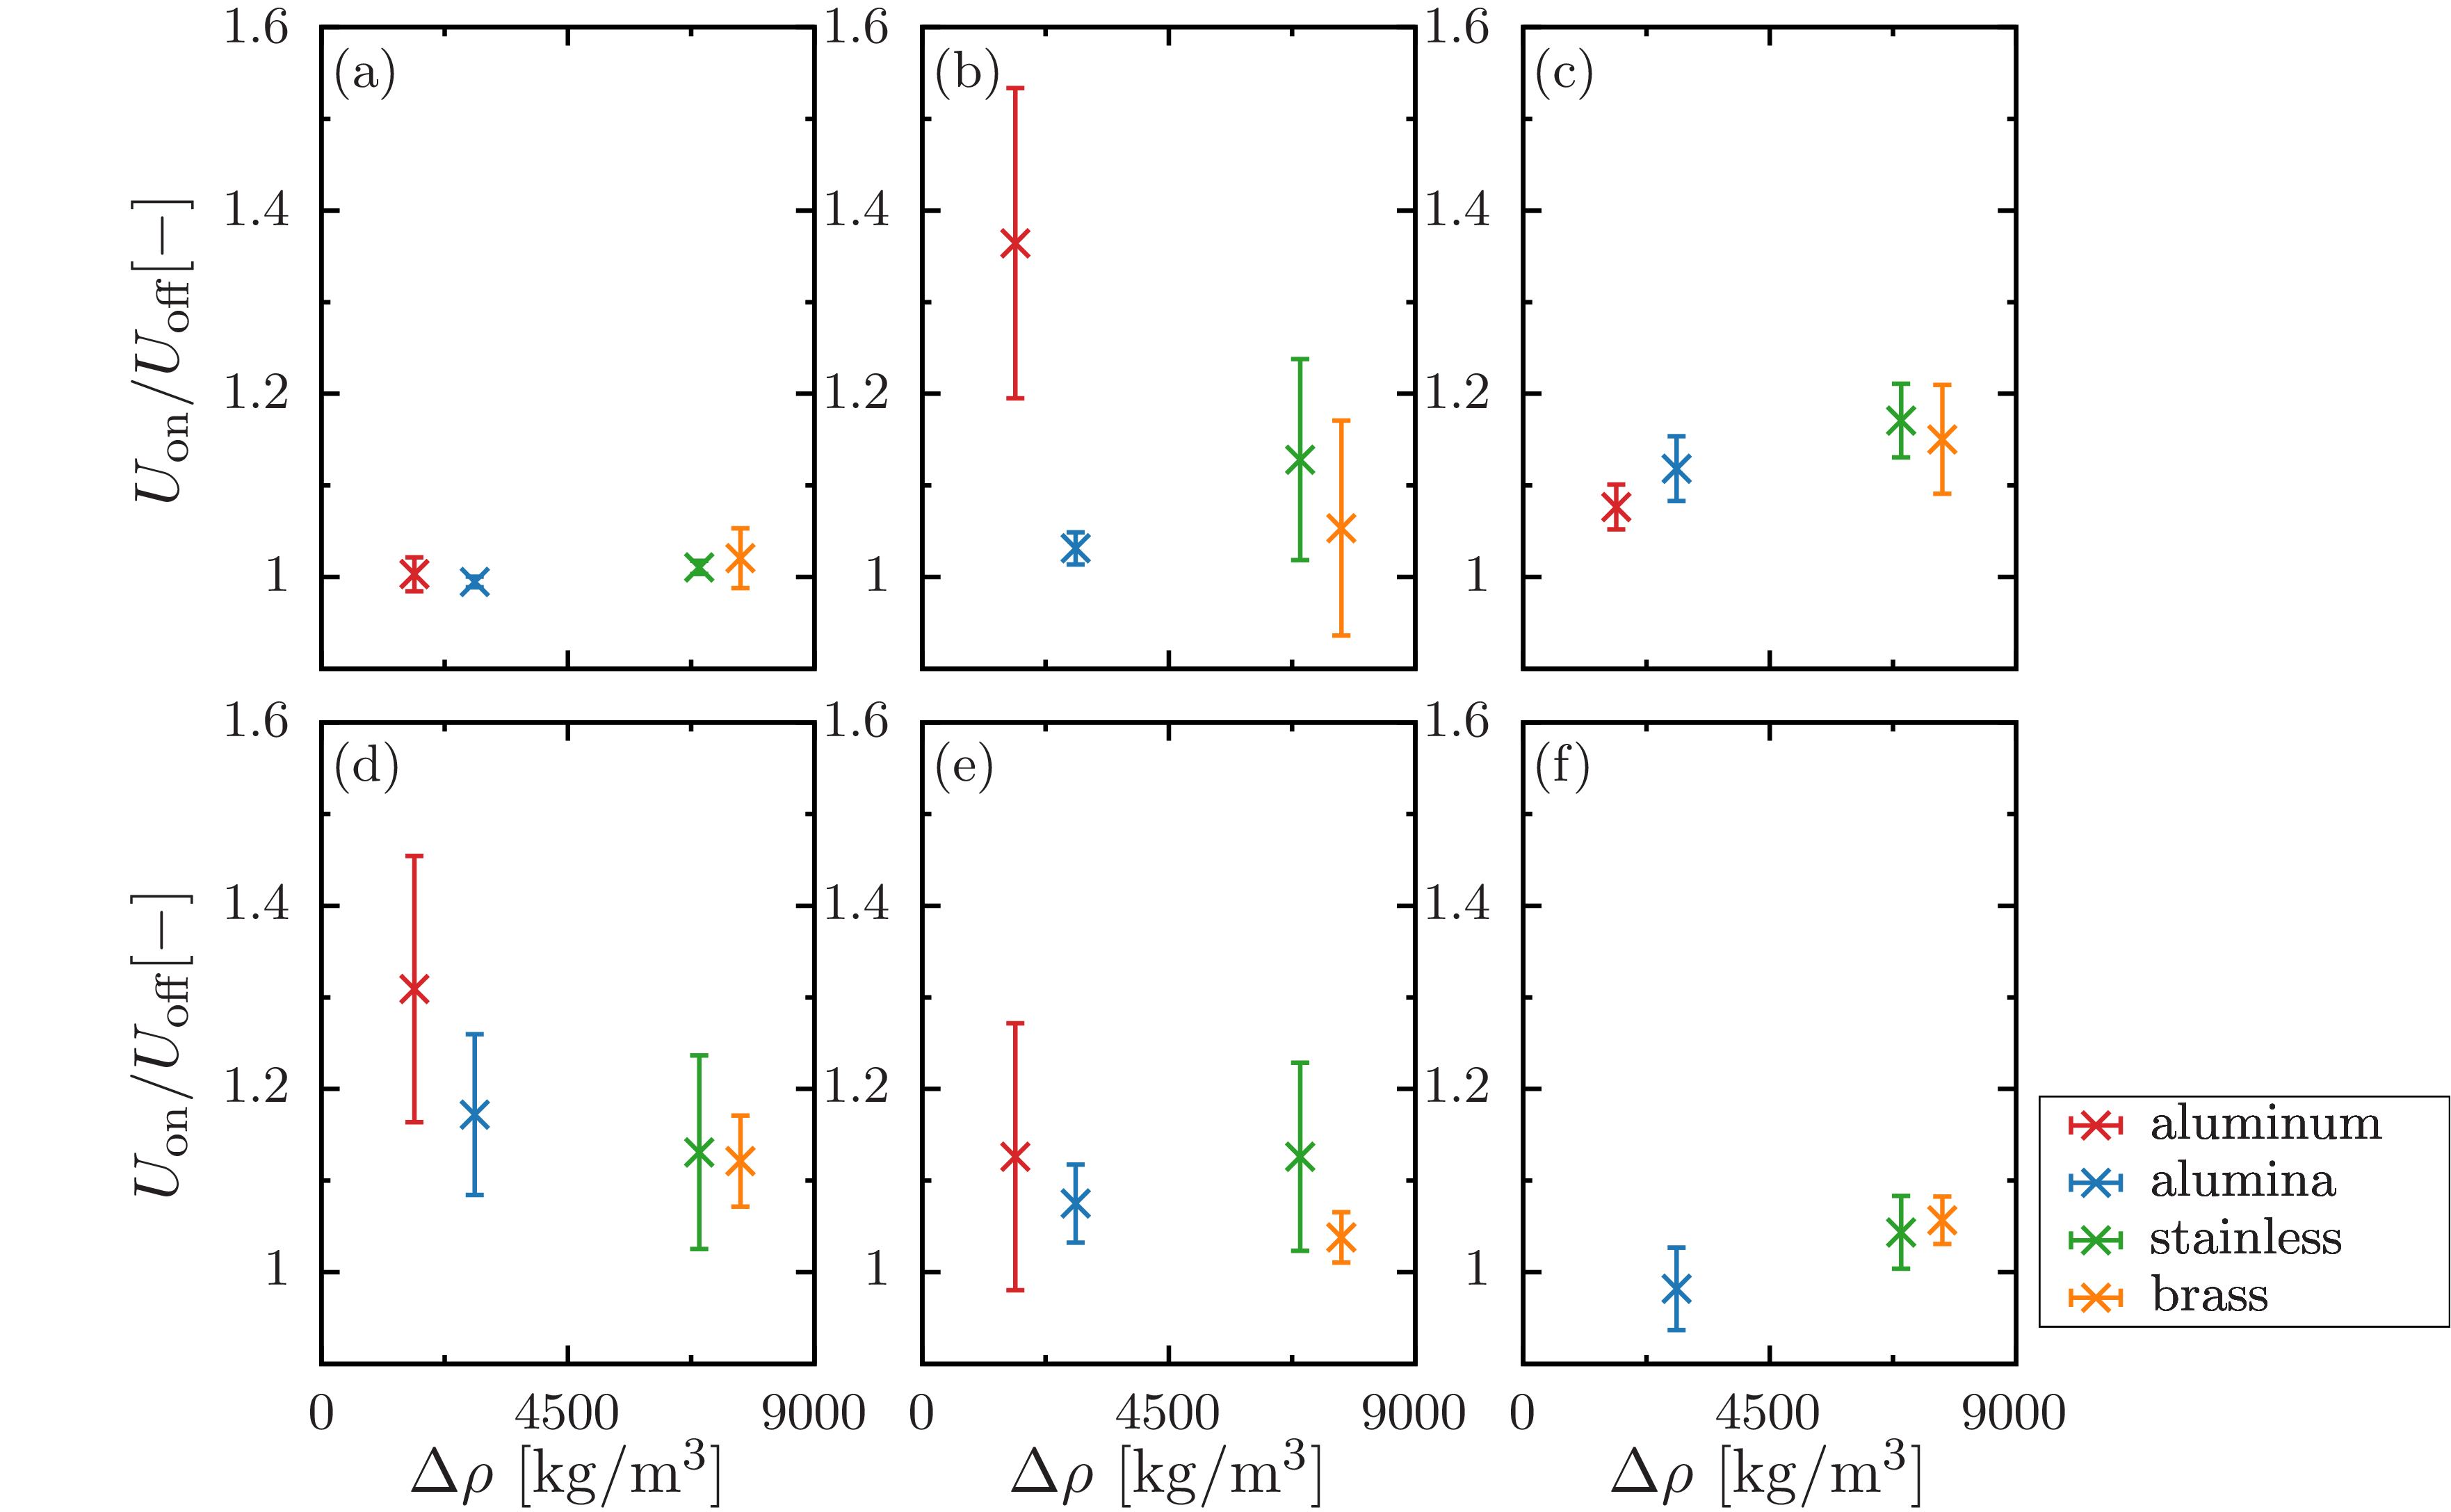
\includegraphics[width=1.0\textwidth]{./5-Results/density/rhoUdiff.png}
    \caption{Velocity ratio by density difference in PAA solution (a)0.2wt.\%, (b)0.5wt.\%, (c)0.7wt.\%, (d)1.0wt.\%, (e)1.3wt.\%, (f)1.5wt.\%.}
    \label{fig:rhoUdiff}
\end{figure}

\begin{figure}[ht]
    \centering
    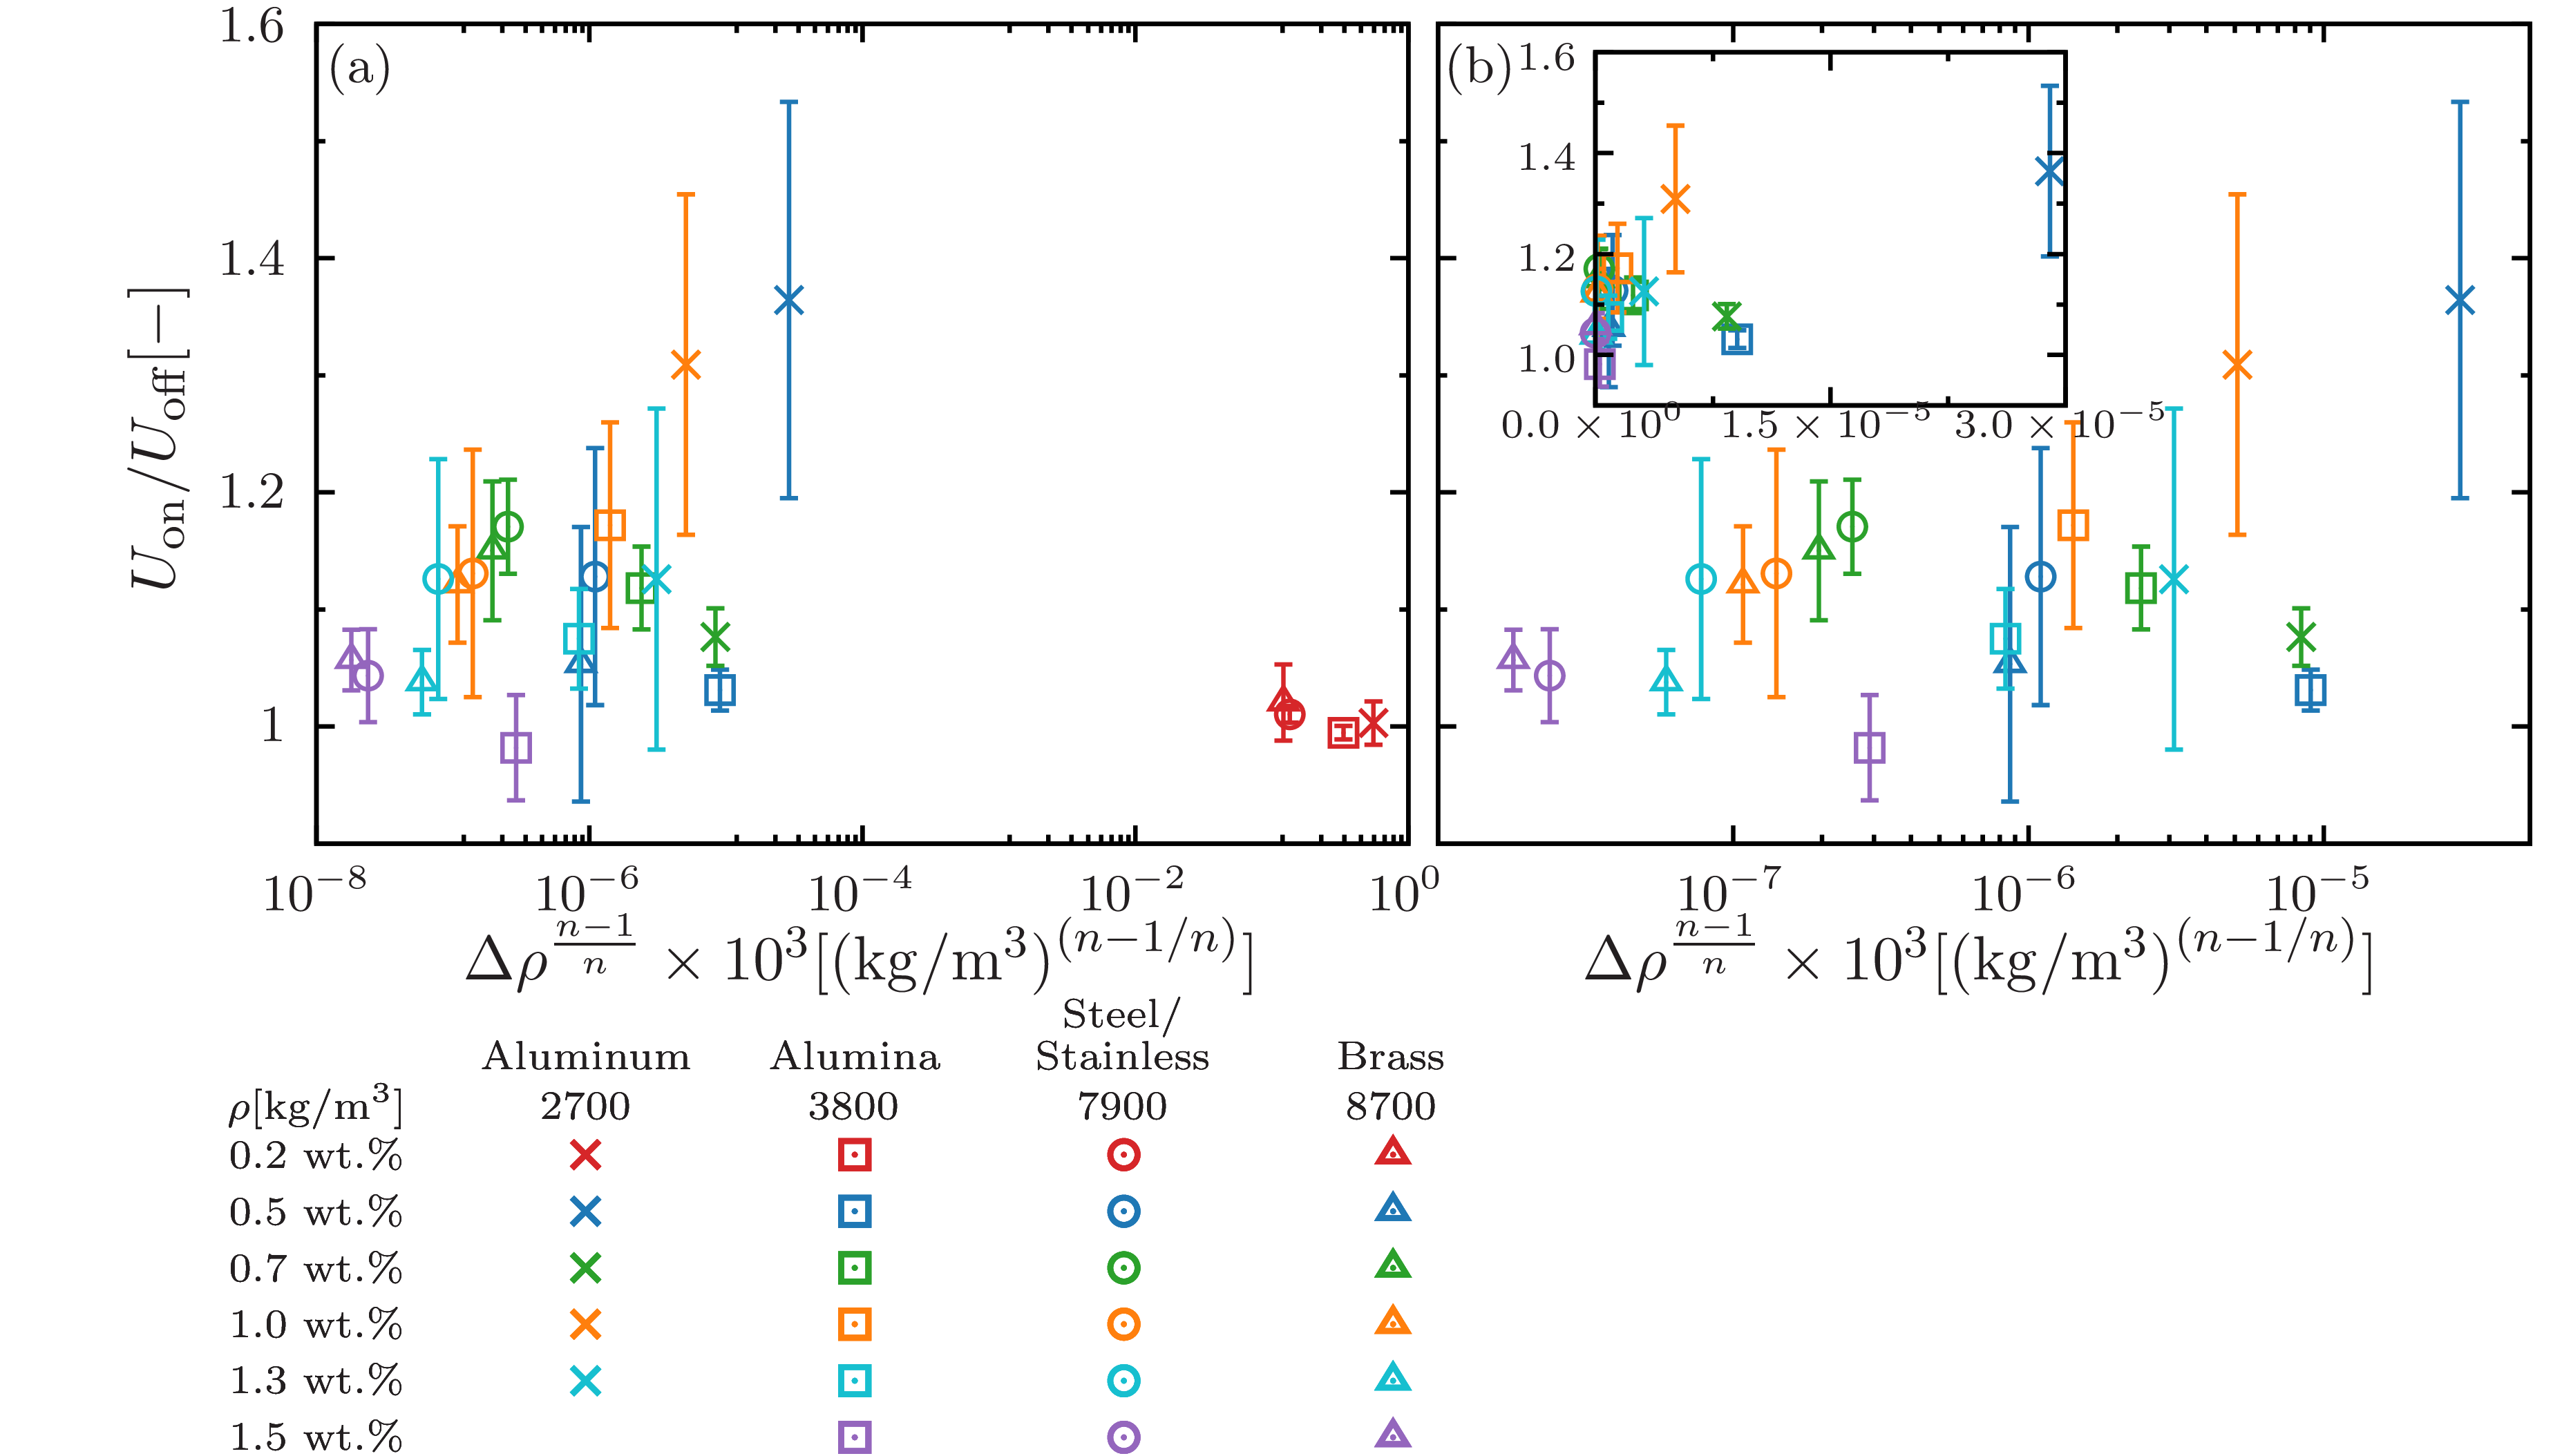
\includegraphics[width=1.0\textwidth]{./5-Results/density/rhoUdiffAll.png}
    \caption{Relationship between density difference and velocity ratio by (a)all data, (b)with out 0.2wt.\% PAA solution data.}
    \label{fig:rhoUdiffAll}
\end{figure}
\clearpage
\section{溶液濃度の影響}

先ほどの節では,密度による落下球高速化への影響を議論したが,本節では溶液濃度による高速化への影響に関して考える.

PAA溶液濃度と終端速度の関係をFig.\ref{fig:concentrationUT}に示す.溶液濃度が濃くなると,終端速度が遅くなることが分かった.PAA溶液濃度と高速化度合の関係をFig.\ref{fig:concentrationUdiff}に示す.縦軸は高速化度合$U_\text{on}/U_\text{off}$,横軸はPAA溶液濃度である.アルミニウム,アルミナにおいてはPAA濃度1wt.\%をピークとして高速化が見られた.一方でステンレスは明瞭な高速化のピークが見られなかったが,PAA濃度0.7-1.3wt.\%のいずれかに高速化のピークが存在すると考えられる.また,真鍮においてPAA濃度0.7wt.\%をピークとして高速化が見られた.これらより,濃度が濃くなると高速化が顕著になるが,濃すぎると高速化がみられにくくなることが分かった.

式(\ref{eq:UdiffRho})を用いて,落下球の密度,溶液濃度の影響を整理した結果をFig.\ref{fig:concentrationUdiffAll}に示す.先述のFig.\ref{fig:rhoUdiffAll}よりも弱い正の相関がみられた.落下球の高速化に対して,粘性による影響よりも密度による影響がより大きいと分かった.

\begin{figure}[ht]
    \centering
    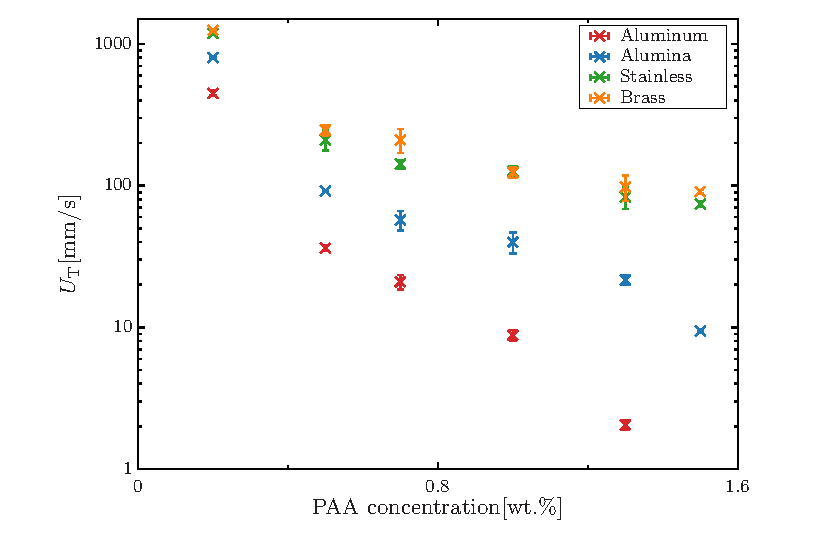
\includegraphics[width=0.8\textwidth]{./5-Results/concentrationUT.eps}
    \caption{Termination velocity in PAA solution concentration.}
    \label{fig:concentrationUT}
\end{figure}

\begin{figure}[ht]
    \centering
    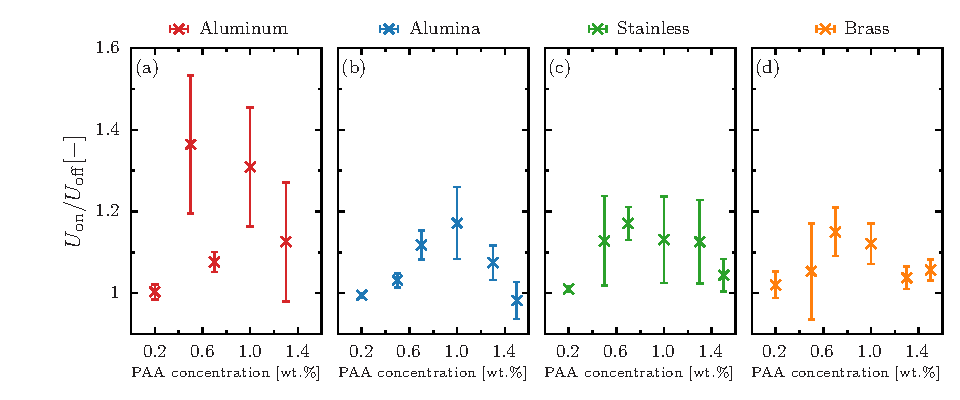
\includegraphics[width=1.0\textwidth]{./5-Results/concentrationUdiff.eps}
    \caption{Velocity ratio in PAA solution concentration (a)Aluminum, (b)Alumina, (c)Stainless, (d)Brass.}
    \label{fig:concentrationUdiff}
\end{figure}

\begin{figure}[ht]
    \centering
    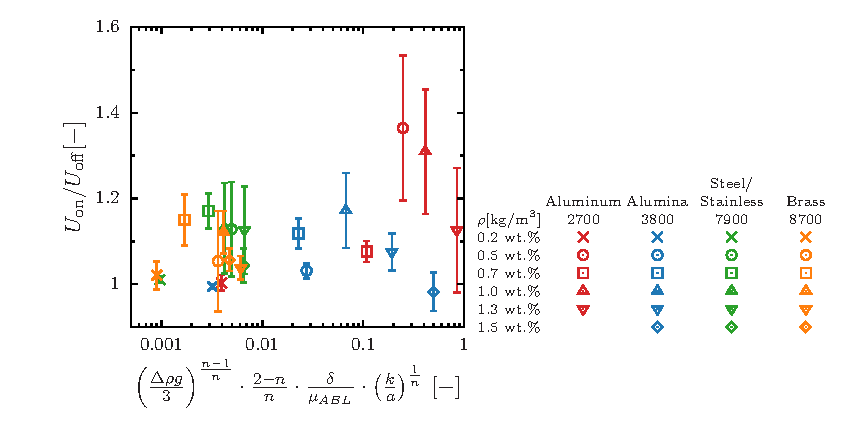
\includegraphics[width=1.0\textwidth]{./5-Results/concentrationUdiffAll.eps}
    \caption{Relationship between density, viscosity and terminal velocity.}
    \label{fig:concentrationUdiffAll}
\end{figure}
\clearpage
\section{高速化に対する球径の影響}
\label{sec:diameter}
先行研究より拡張した領域における球径による影響を考えるため,異なる寸法の鋼球を用いて落下球実験を行った.先行研究に比べて,広いパラメータ範囲で実験条件(Table\ref{table:exp-conditions-dia})を定めた.媒質の質量濃度ごとに球径による高速化への影響を検討する.

\subsection{PAA1.0wt.\%の場合}
PAA1.0wt.\%における球径変化の実験結果をFig\ref{fig:diameter}に示す.その結果より,落下球の直径と終端速度の関係をFig\ref{fig:diaUT}(a)に示す.落下球の直径が大きくなると,終端速度が指数関数的に高速化した.また,直径と超音波照射による高速化度合の関係をFig\ref{fig:diaUT}(b)に示す.落下球の直径10mmをピークとして超音波照射による高速化が見られた.

これらより,式(\ref{eq:Udiff})を用いて整理した結果をFig\ref{fig:muUdiff}に示す.Fig\ref{fig:muUdiff}(a)においては先行研究\cite{ref:8}の実験結果全範囲を,Fig\ref{fig:muUdiff}(b)においては今回の実験結果によって得られた範囲を拡大した結果を示す.落下球の直径10mm以上において,粘度比と音響境界層を球の半径で規格化した値は,超音波照射による球の高速化度合いに対して正の相関関係にあった.一方で先行研究\cite{ref:8}において示された範囲では,高速化が抑制され非常に小さな値となっていた.先行研究\cite{ref:8}では,この抑制が弾性影響に由来することが示唆されている.弾性影響は第\ref{sec:elasticity-discussion}章で,議論する.

\begin{figure}[ht]
    \centering
    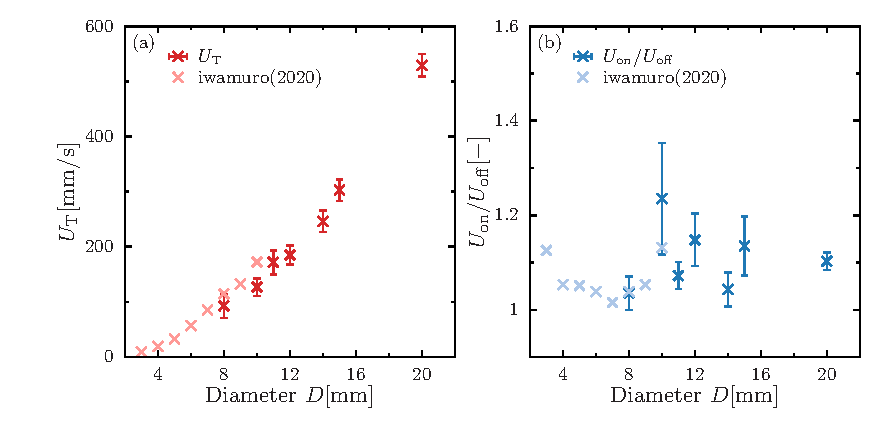
\includegraphics[width=1\textwidth]{./5-Results/diaUT_Udiff.eps}
    \caption{Relationship between diameter and (a)terminal velocity, (b)velocity rato.}
    \label{fig:diaUT}
\end{figure}

\begin{figure}[ht]
    \centering
    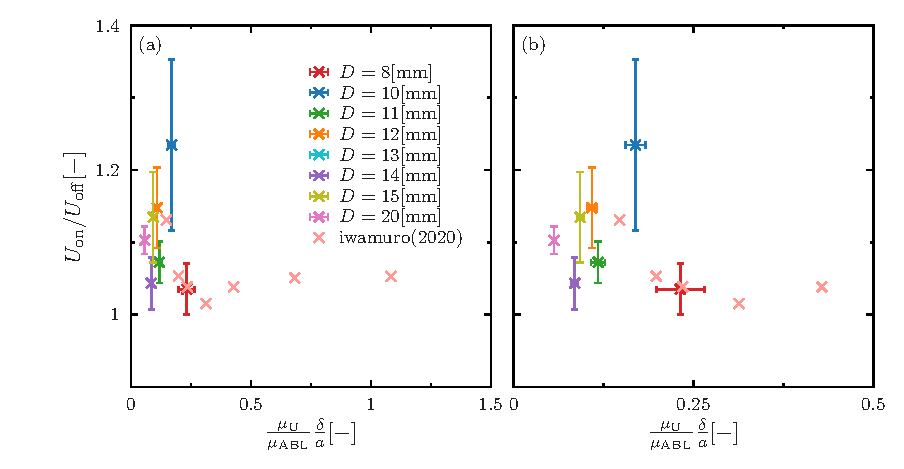
\includegraphics[width=1\textwidth]{./5-Results/mu_Udiff.eps}
    \caption{Relationship between velocity rato and viscosity ratio, the acoustic boundary layer thickness, radius (a)with Iwamuro (2020), (b)without Iwamuro (2020).}
    \label{fig:muUdiff}
\end{figure}

\newpage

\subsection{PAA0.5wt.\%の場合}
PAA0.5wt.\%における球径変化の実験結果をFig\ref{fig:diameter-0.5}に示す.その結果より,落下球の直径と終端速度の関係をFig\ref{fig:diaUT0.5}(a)に示す.落下球の直径が大きくなると,PAA1wt.\%の場合と同様に終端速度が指数関数的に高速化した.また,直径と超音波照射による高速化度合いの関係をFig\ref{fig:diaUT0.5}(b)に示す.PAA1wt.\%の場合と同様に落下球の直径10mmをピークとして超音波照射による高速化が見られた.

式(\ref{eq:Udiff})を用いて高速化度合を整理した結果をFig\ref{fig:muUdiff0.5}に示す.落下球の直径が10mm以上において粘度比と音響境界層を球の半径で規格化した値は,超音波照射による球の高速化度合いに対して正の相関関係にあった.一方で,直径5mmの落下球は高速化度合いが非常に小さくなった.このことに関して,他の結果も含めて,本研究\ref{sec:viscosity},\ref{sec:elasticity-discussion}章にて,議論を行う.
\begin{figure}[ht]
    \centering
    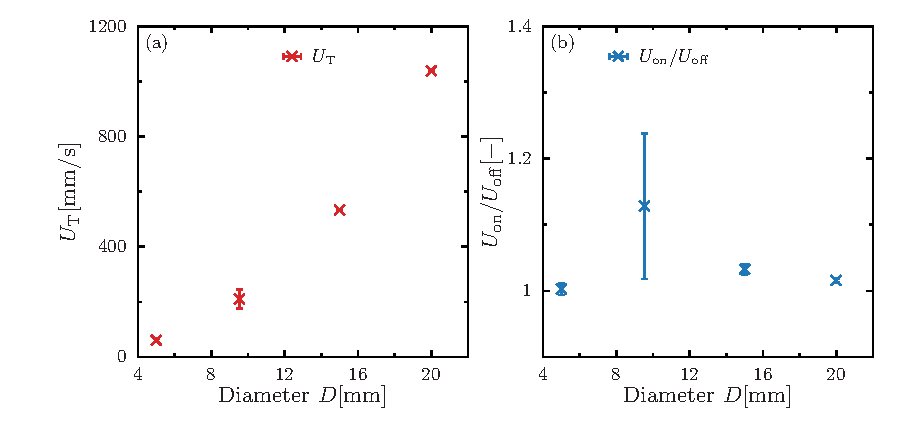
\includegraphics[width=1\textwidth]{./5-Results/diameter-0.5/diaUT_Udiff.eps}
    \caption{Relationship between diameter and (a)terminal velocity, (b)velocity rato.}
    \label{fig:diaUT0.5}
\end{figure}

\begin{figure}[ht]
    \centering
    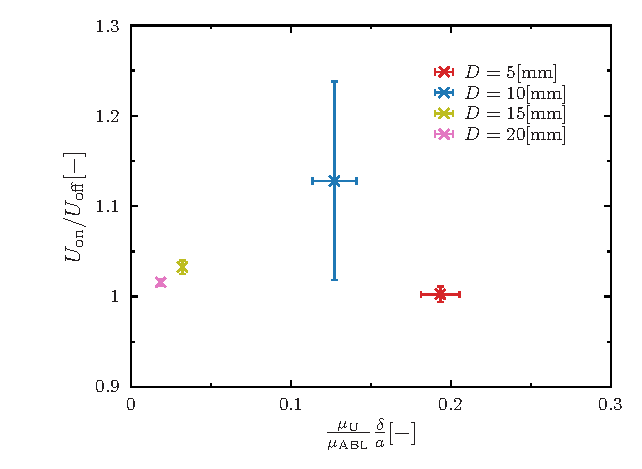
\includegraphics[width=0.8\textwidth]{./5-Results/diameter-0.5/mu_Udiff.eps}
    \caption{Relationship between velocity rato and viscosity ratio, the acoustic boundary layer thickness, radius.}
    \label{fig:muUdiff0.5}
\end{figure}

\clearpage

\subsection{PAA0.2,1.3wt.\%の場合}
PAA0.2,1.3wt.\%における球径変化の実験結果をFig\ref{fig:diameter-0.2-1.3}に示す.その結果より,落下球の直径と終端速度の関係をFig\ref{fig:diaUT0.2-1.3}(a)に示す.落下球の直径が大きくなると,他の質量濃度と同様に終端速度が高速化した.また,直径と超音波照射による高速化度合いの関係をFig\ref{fig:diaUT0.2-1.3}(b)に示す.PAA0.2wt.\%において,顕著な高速化は見られなかった.一方で,PAA1.3wt.\%において,落下球の直径が小さい場合に高速化が見られた.

式(\ref{eq:Udiff})を用いて高速化度合いを整理した結果をFig\ref{fig:muUdiff0.2-1.3}に示す.粘度比と音響境界層厚さを球の半径で規格化した値は,超音波照射による球の高速化度合いに対して正の相関関係にあった.他の結果も含めて,本研究\ref{sec:viscosity},\ref{sec:elasticity-discussion}章にて,より詳しい議論を行う.

\begin{figure}[ht]
    \centering
    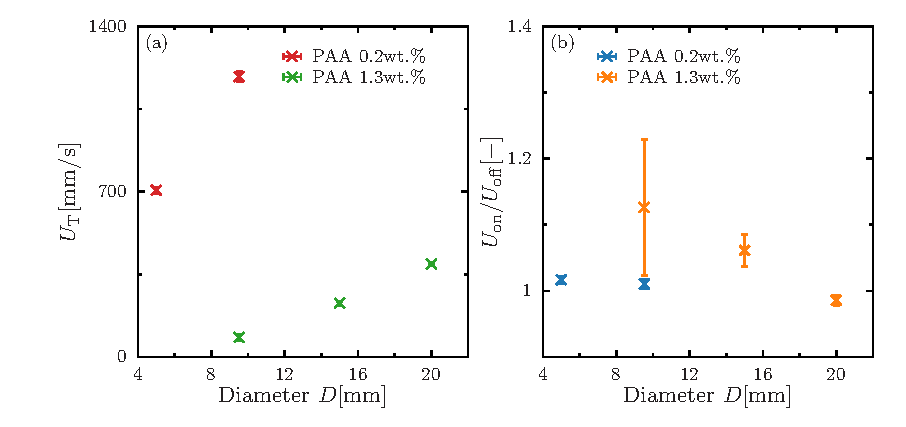
\includegraphics[width=0.9\textwidth]{./5-Results/diameter-0.2-1.3/diaUT_Udiff.eps}
    \caption{Relationship between diameter and (a)terminal velocity, (b)velocity rato.}
    \label{fig:diaUT0.2-1.3}
\end{figure}

\begin{figure}[ht]
    \centering
    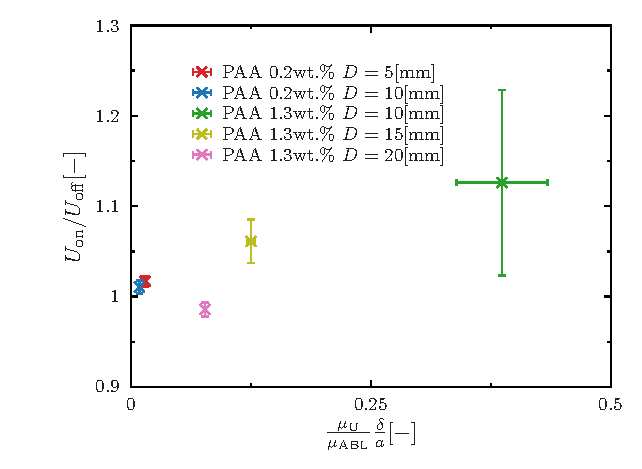
\includegraphics[width=0.7\textwidth]{./5-Results/diameter-0.2-1.3/mu_Udiff.eps}
    \caption{Relationship between velocity rato and viscosity ratio, the acoustic boundary layer thickness, radius.}
    \label{fig:muUdiff0.2-1.3}
\end{figure}
\clearpage
\section{粘度による整理}

これまでの実験結果を先行研究である岩室\cite{ref:8}で用いられた手法で整理を行う.式(\ref{eq:Udiff})を用い
Fig.\ref{fig:viscosity_ratio}に示す.

\begin{figure}[ht]
    \centering
    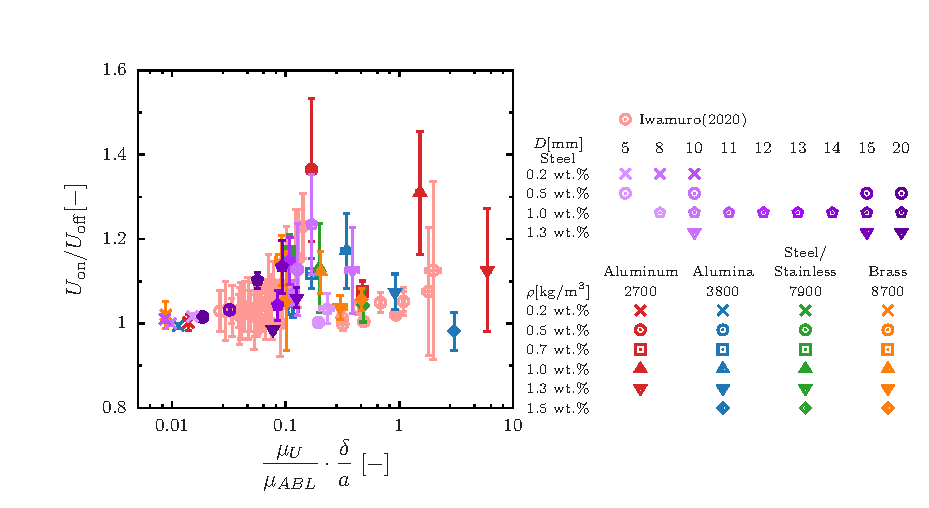
\includegraphics[width=1.0\textwidth]{5-Results/viscosity.eps}
    \caption{}
    \label{fig:viscosity_ratio}
\end{figure}

\clearpage
\section{弾性による影響}

粘性による影響では説明が十分にできない
球の落下によって生じる応力$\tau_\text{U}$に関して,
\begin{eqnarray}
    \tau_U \sim k \times \left(\frac{U_\text{T}}{a}\right),
    \label{eq:tauU}
\end{eqnarray}
といった式で近似できる.この式(\ref{eq:tauU})を用いて,
応力比
Fig.\ref{fig:elastcity}に示す.

\begin{figure}[h]
    \centering
    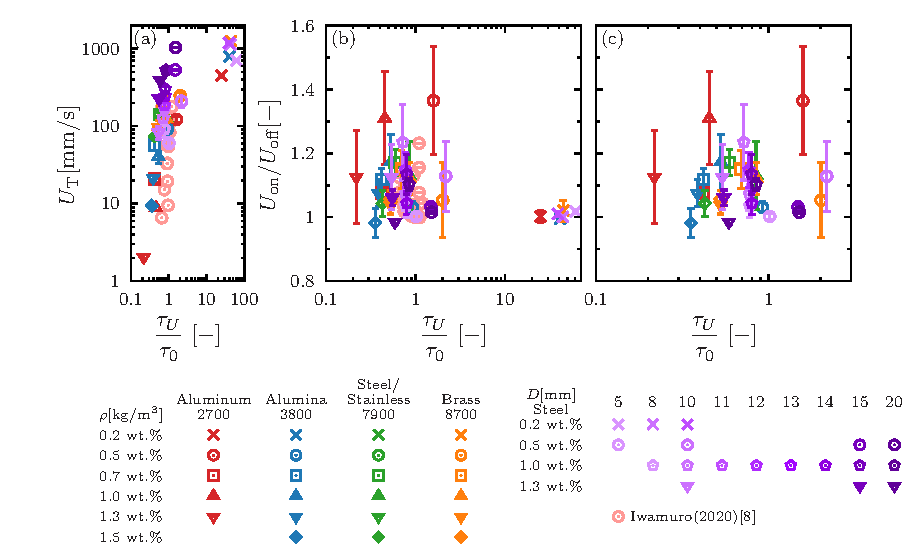
\includegraphics[width=1.0\textwidth]{5-Results/elastcity.eps}
    \caption{Relationship between velocity ratio and elasticity ratio$\tau_\text{U}/\tau_\text{0}$.}
    \label{fig:elastcity}
\end{figure}

\clearpage
\newpage
\clearpage
\section{結言}

今回,従来の落下球の把持方法を変化させ,真空ポンプを用いて球の把持を行った.その結果,電磁石を用いて球の把持をした場合と比較して,落下開始時のオーバーシュートがあまり見られなかった.一方で,真空ポンプを用いて球を把持した場合においても,球に初速を与えた場合,落下開始時にオーバーシュートが見られた.これらを踏まえて,電磁石を用いて球の把持を行った場合,落下開始時に初速を与えていることが分かった.真空ポンプを用いて球の把持を行った場合,初速が存在しないことも分かった.また,落下開始時のオーバーシュートは流体の弾性によるものだが,$De$数を用いることでオーバーシュートの有無を分類することができると分かった.

球の落下間隔を変化させた場合,落下間隔が長くなると,落下速度が遅くなった.これは落下間隔が長くなると,粘弾性の回復が十分にされるためだと分かった.また,球の落下間隔を変化させた場合も音響境界層内の粘度とその厚さによって,超音波照射による高速化が発生していることが分かった.今回は粘性による影響のみを議論したが,落下間隔が長くなると,落下開始時にオーバーシュートといった弾性による影響も見られた.このことより,弾性による影響も調査する必要があると考えられる.


\newpage
\begin{appendices}
	\section{球落下実験 実験結果}
\label{sec:expData}

\subsection{密度・濃度による影響に関して}
本研究において,落下させる球の密度,擬塑性流体の質量濃度を変化させた.それぞれの質量濃度における,球の落下速度をFig.\ref{fig:0.05-0.2}-\ref{fig:1.5}に示す.横軸は経過時間[s],縦軸は落下速度[m/s]である.

\begin{figure}[h]
    \centering
    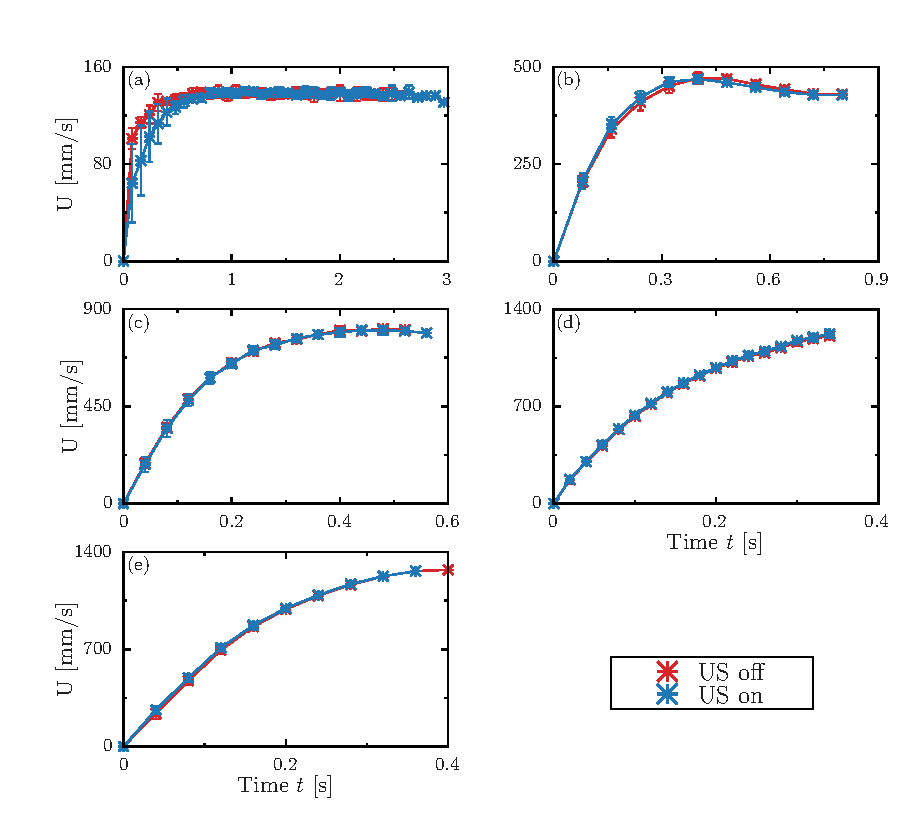
\includegraphics[width=1.0\textwidth]{5-Results/0.05-0.2.eps}
    \caption{Velocity of a falling sphere made by (a)nylon in 0.05 wt.\% PAA solution, (b)aluminum, (c)alumina, (d)stainless,(e)brass in 0.2 wt.\% PAA solution.}
    \label{fig:0.05-0.2}
\end{figure}

\begin{figure}[h]
    \centering
    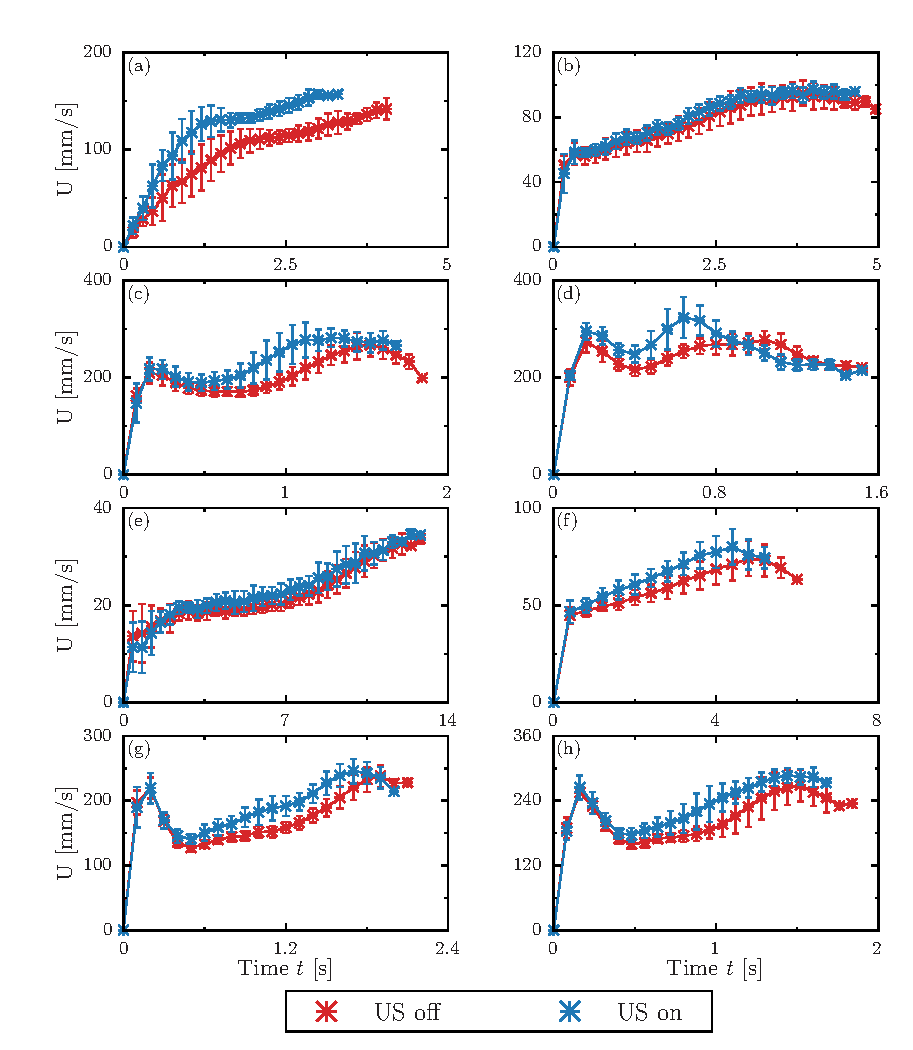
\includegraphics[width=1.0\textwidth]{5-Results/0.5-0.7.eps}
    \caption{Velocity of a falling sphere made by (a)aluminum, (b)alumina, (c)stainless,(d)brass in 0.5 wt.\% PAA solution, (e)aluminum, (f)alumina, (g)stainless,(h)brass in 0.7 wt.\% PAA solution.}
    \label{fig:0.5-0.7}
\end{figure}

\begin{figure}[h]
    \centering
    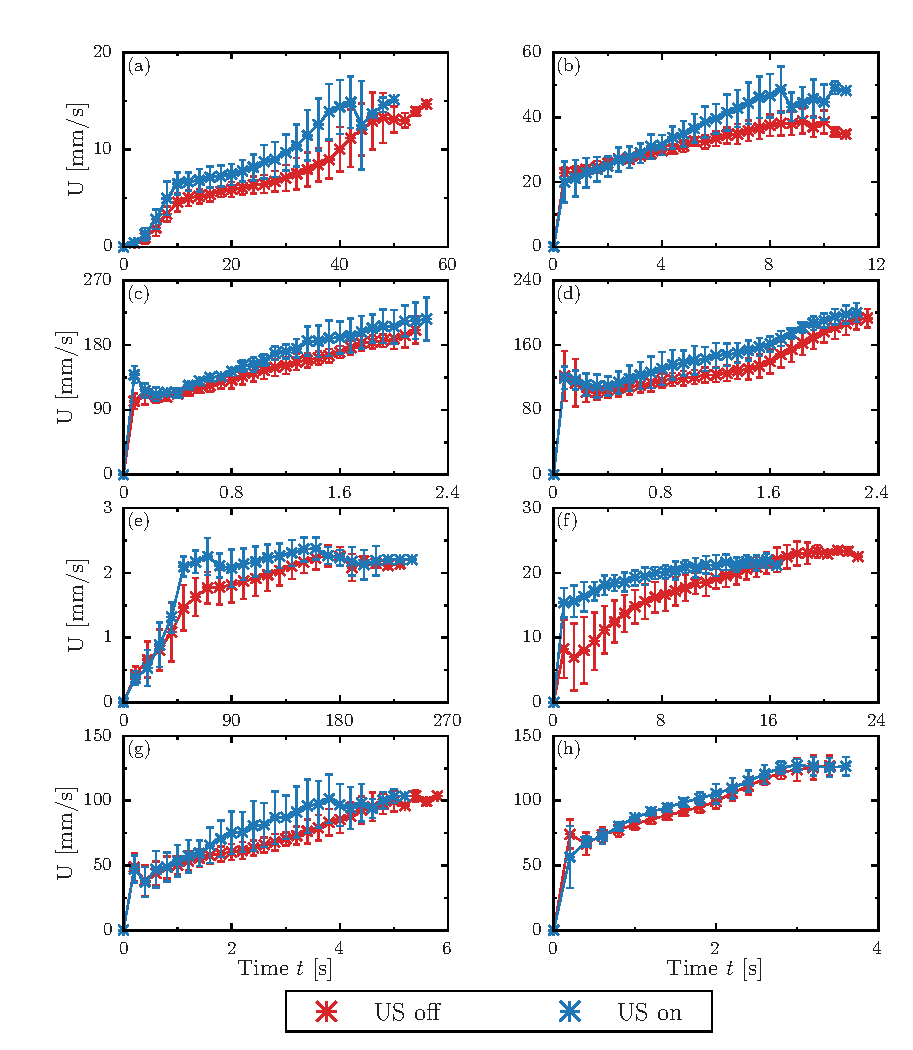
\includegraphics[width=1.0\textwidth]{5-Results/1.0-1.3.eps}
    \caption{Velocity of a falling sphere made by (a)aluminum, (b)alumina, (c)stainless,(d)brass in 1.0 wt.\% PAA solution, (e)aluminum, (f)alumina, (g)stainless,(h)brass in 1.3 wt.\% PAA solution.}
    \label{fig:1.0-1.3}
\end{figure}

\begin{figure}[h]
    \centering
    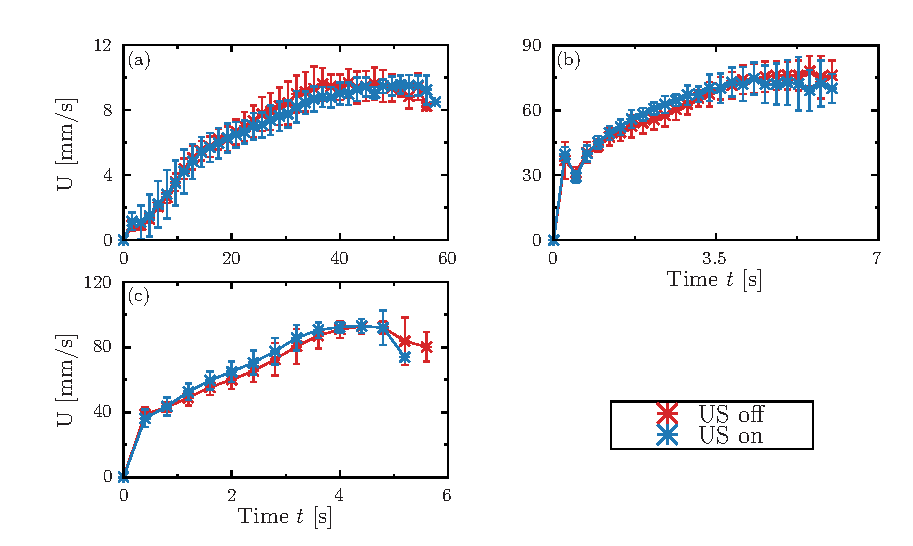
\includegraphics[width=1.0\textwidth]{5-Results/1.5.eps}
    \caption{Velocity of a falling sphere made by (a)alumina, (b)stainless,(c)brass in 1.5 wt.\% PAA solution.}
    \label{fig:1.5}
\end{figure}

\clearpage

\subsection{球径による影響に関して}

球径を変化させた際の実験結果をFig.\ref{fig:diameter}-\ref{fig:diameter-0.2-1.3}に示す.横軸は経過時間[s],縦軸は落下速度[m/s]である.

\begin{figure}[h]
    \centering
    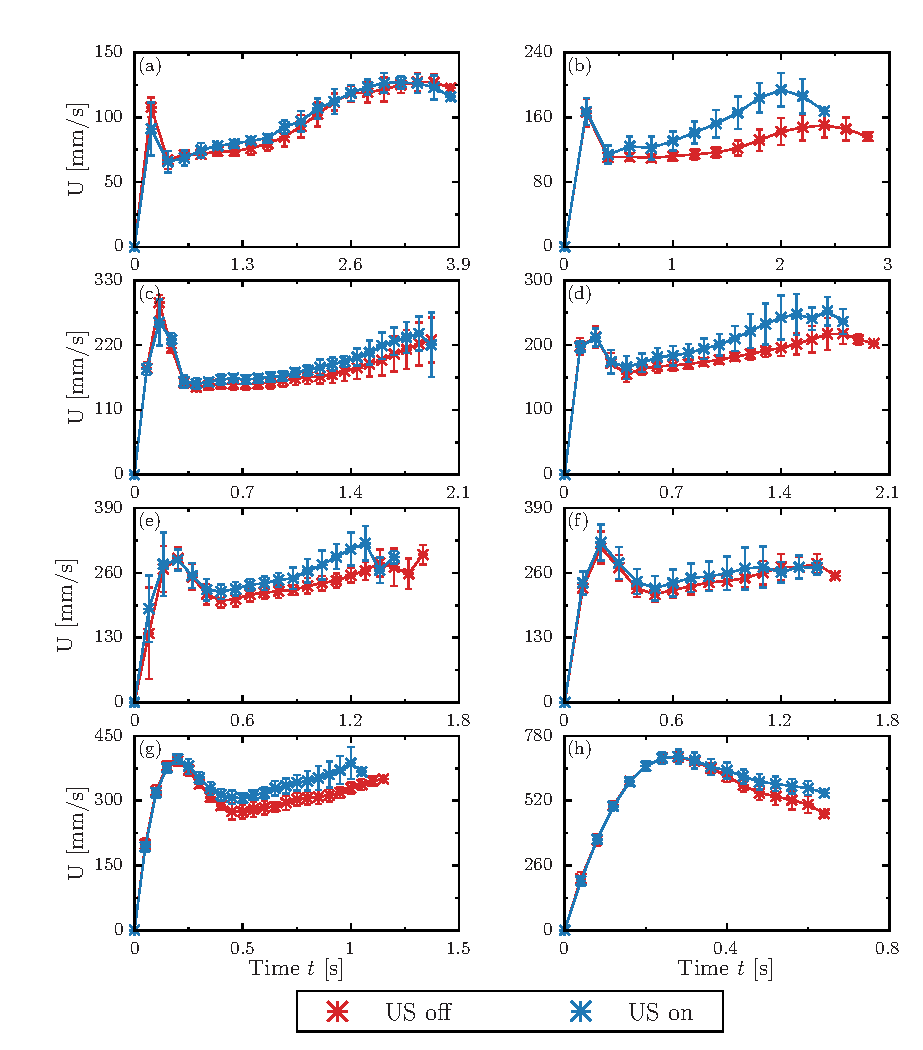
\includegraphics[width=0.9\textwidth]{X-Appendix/diameter/diameter.eps}
    \caption{Velocity of a falling sphere in 1.0wt.\% PAA of (a)8mm, (b)10mm, (c)11mm, (d)12mm, (e)13mm, (f)14mm, (g)15mm, (h)20mm.}
    \label{fig:diameter}
\end{figure}

\begin{figure}[h]
    \centering
    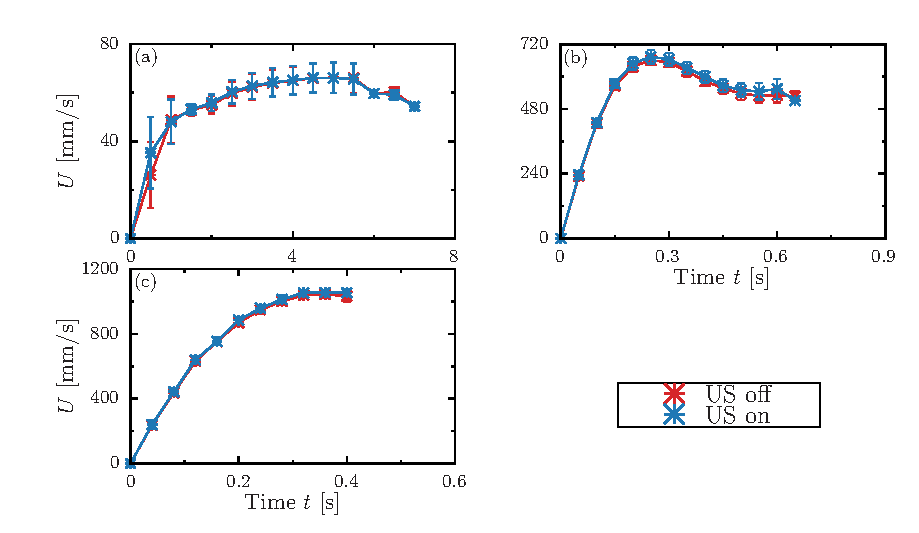
\includegraphics[width=1\textwidth]{X-Appendix/diameter-0.5/diameter.eps}
    \caption{Velocity of a falling sphere in 0.5wt.\% PAA of (a)5mm, (b)15mm, (c)20mm.}
    \label{fig:diameter-0.5}
\end{figure}

\begin{figure}[h]
    \centering
    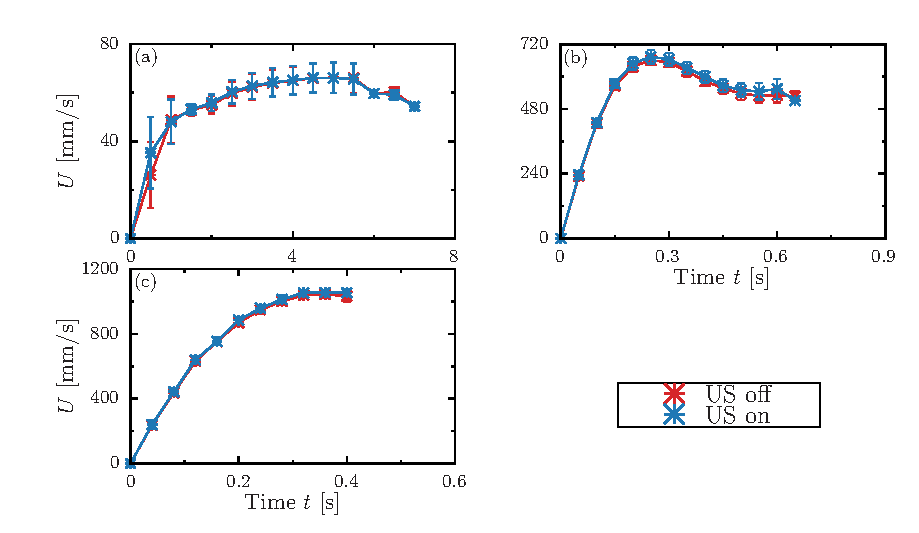
\includegraphics[width=1\textwidth]{X-Appendix/diameter-0.5/diameter.eps}
    \caption{Velocity of a falling sphere in (a)0.2wt.\% PAA of 5mm, 1.3wt.\% PAA of (b)15mm, (c)20mm.}
    \label{fig:diameter-0.2-1.3}
\end{figure}

	\clearpage
	\section{実験装置の改良による影響}
\label{sec:reexp}
先行研究\cite{ref:8}において,電磁石を用いて,磁力によって球の把持を行っていた.本研究において,強磁性体以外の球の把持を行うため,真空ポンプを用いて吸引する手法に変更した.その把持手法の変化に伴う影響を議論する.

\subsection{実験装置}

電磁石を用いた実験装置をFig.\ref{fig:magnet_device}に示す.電磁石の磁力によって落下球の把持を行った.球を落下させるとき,電磁石への通電を切り,落下方向に力を加えて球を落下させた.また,本実験は先行研究と同様の条件で行うため,外寸において高さ248.5mm,幅47mm,奥行き47mm,厚さ3.5mmの矩形ガラス水槽で実験を行った.また,照射する超音波の周波数は39kHzとした.

\begin{figure}[H]
    \centering
    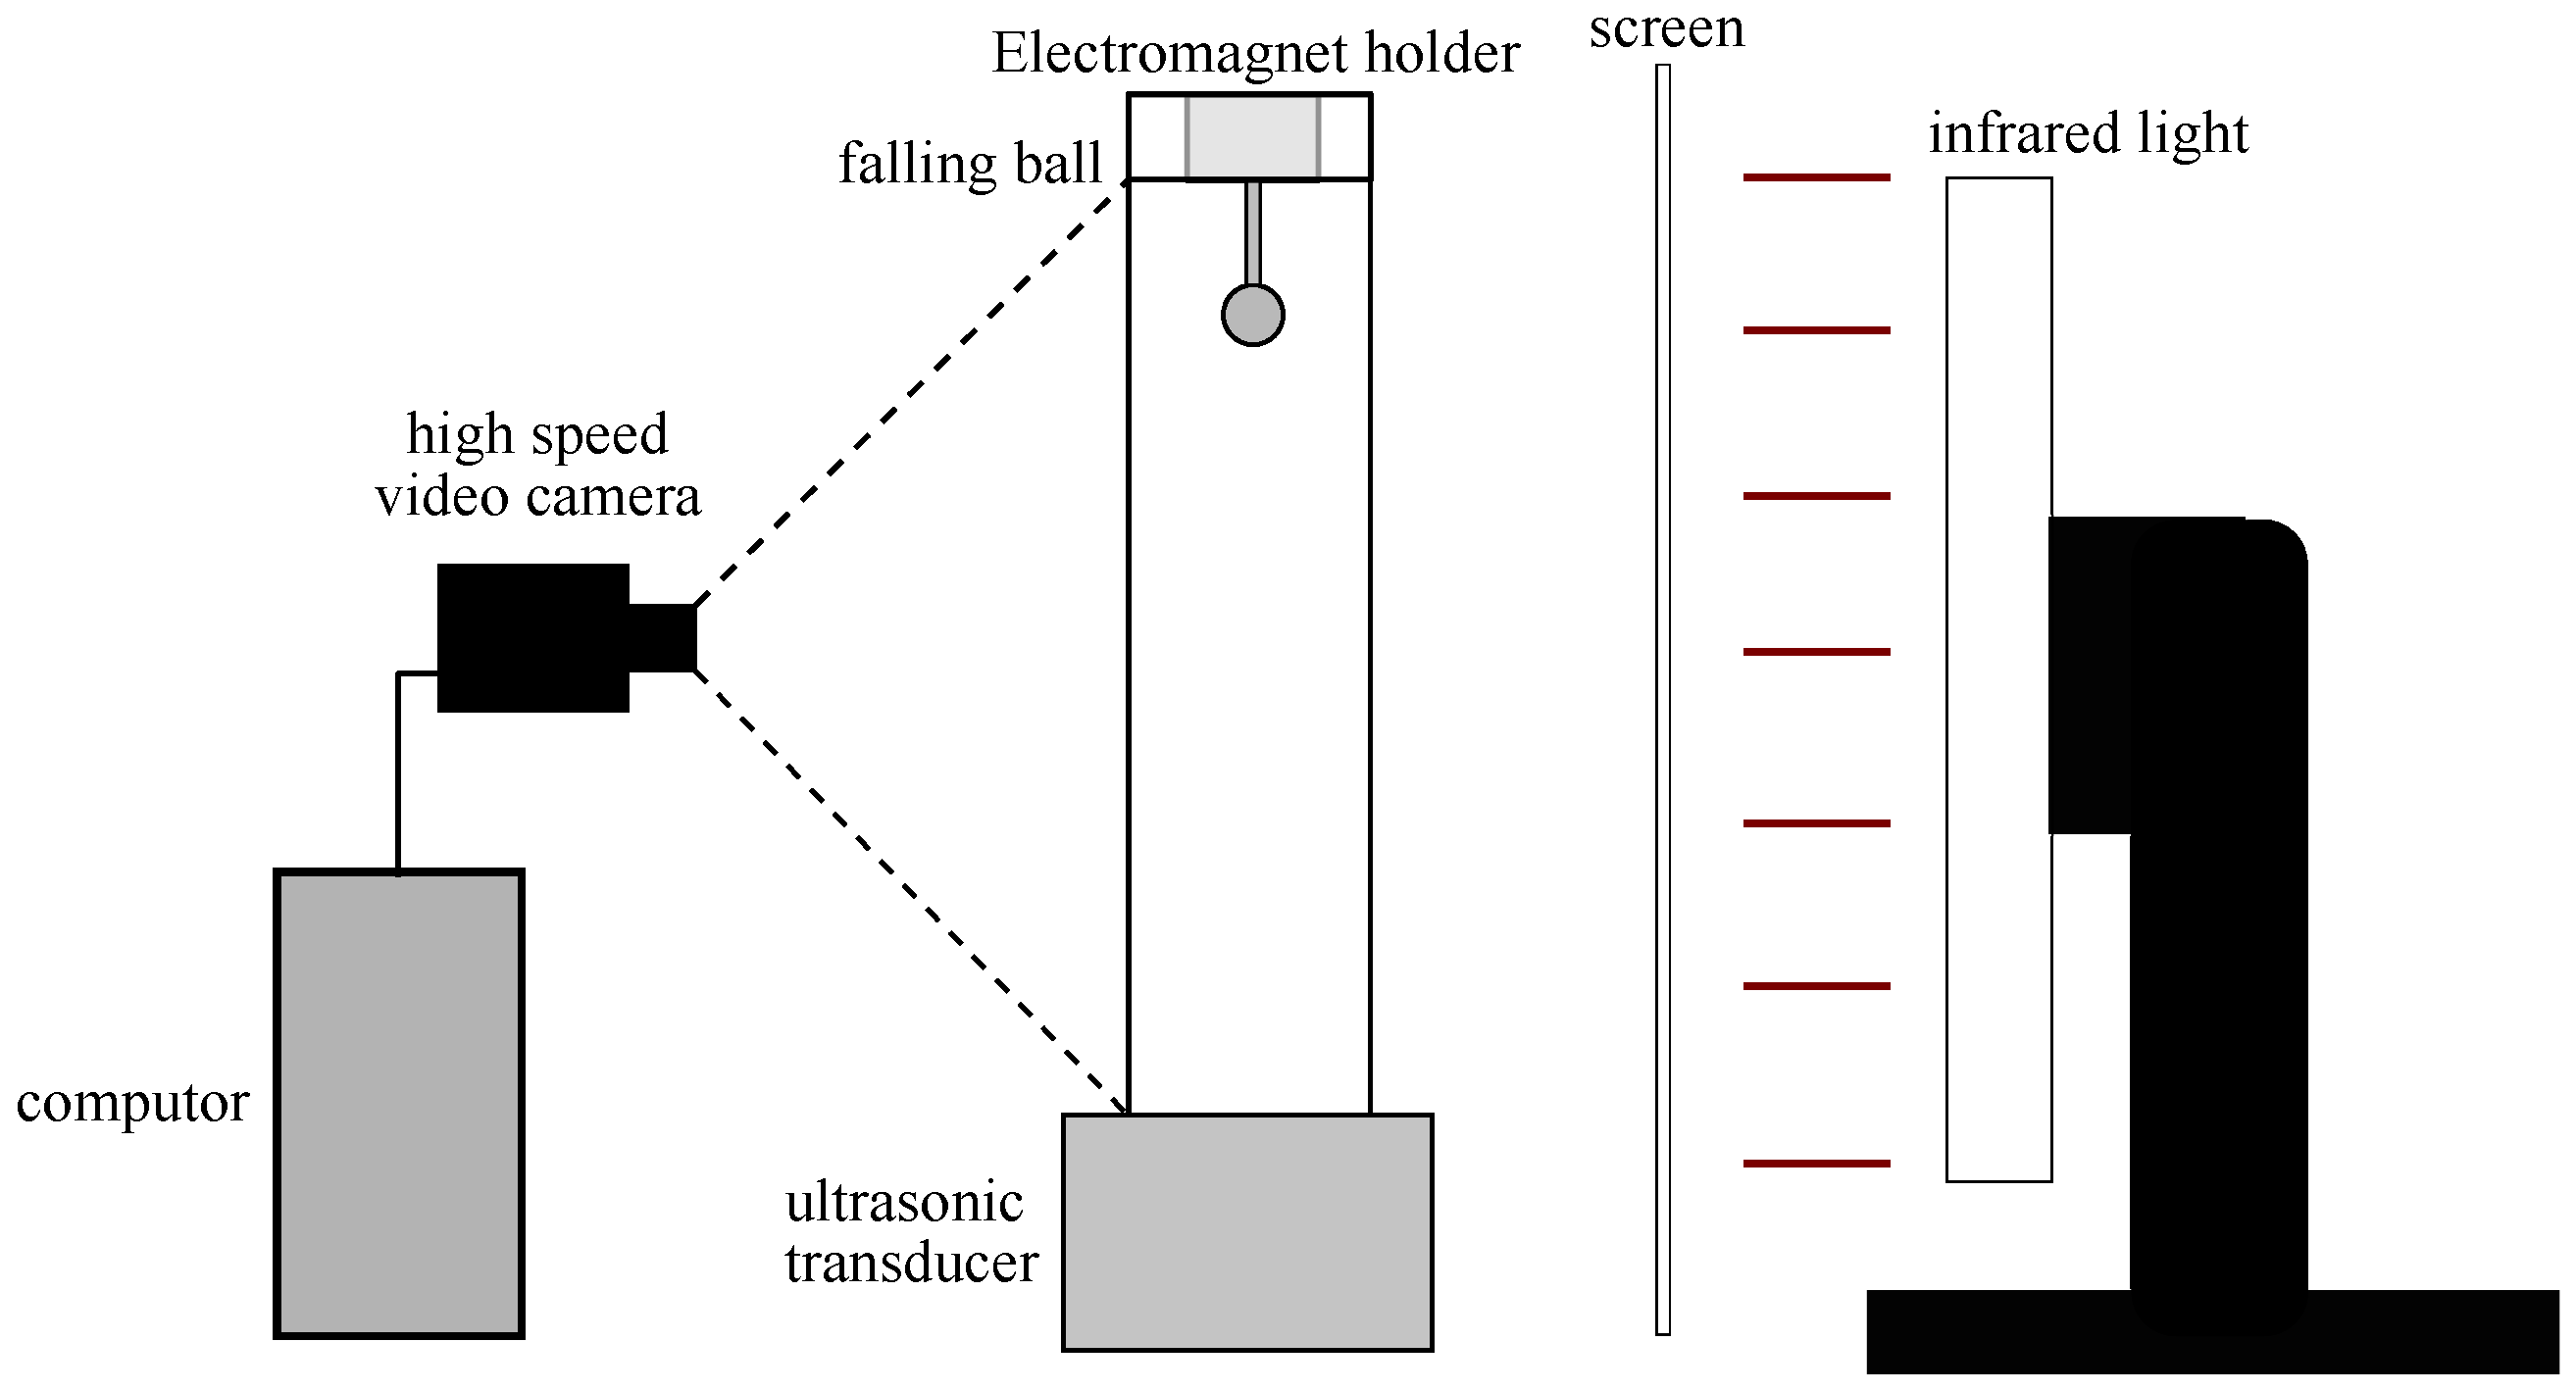
\includegraphics[width=0.95\textwidth]{X-Appendix/device/magnet_device.eps}
    \caption{Schematic view of the experimental apparatus by using electromagnet.}
    \label{fig:magnet_device}
\end{figure}

\subsection{落下実験結果}
真空ポンプを用いて球を把持した場合と電磁石を用いて球を把持した場合の結果をFig \ref{fig:falling-A}に示す.縦軸は落下速度,横軸は落下開始時からの経過時間である.落下開始時に電磁石を用いた場合はオーバーシュートが見られるが,真空ポンプを用いた場合はオーバーシュートが見られなかった.これは,落下開始時における初速による影響が考えられる.本研究\ref{sec:interval-velocity}章にて,初速を与えた場合に関して考える.

終端速度と高速化度合の関係をFig\ref{fig:falling-Udiff}(a)に示す.縦軸は高速化度合,横軸は落下球の終端速度である.真空ポンプを用いて球を把持した場合,先行研究である岩室\cite{ref:8}や電磁石を用いて球を把持した場合と比較し,超音波照射による高速化が顕著に現れなかった.また,粘度比と音響境界層を球の半径で規格化した値と高速化度合の関係をFig.\ref{fig:falling-Udiff}(b)に示す.真空ポンプを用いて把持した場合,粘度比と音響境界層を球の半径で規格化した値が0.1を超える領域に存在する.これは,本研究\ref{sec:viscosity}章で示した高速化があまり見られなくなる領域となっており,真空ポンプを用いて把持した場合,高速化があまり見られていない.先行研究である岩室\cite{ref:8}と今回の実験結果に差異が生じた理由は,作製した溶液の特性や音響圧の違いによって生じたと考えられる.
\begin{figure}[H]
    \centering
    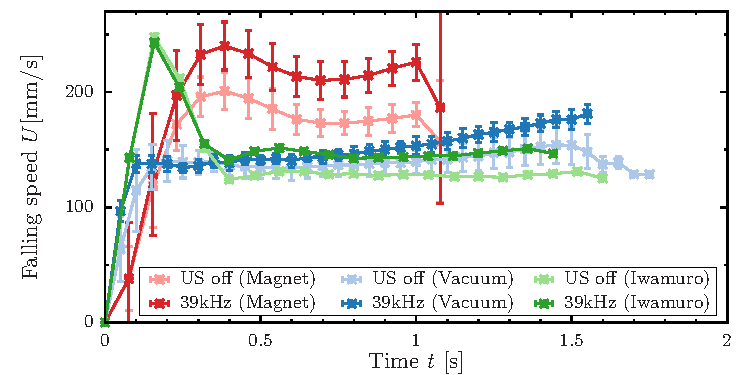
\includegraphics[width=1\textwidth]{./X-Appendix/magnet_vacuum/magnet_vacuum.eps}
    \caption{Falling speed of a sphere in 1.0wt.\%PAA solution with and without ultrasound irradiation.}
    \label{fig:falling-A}
\end{figure}

\begin{figure}[H]
    \centering
    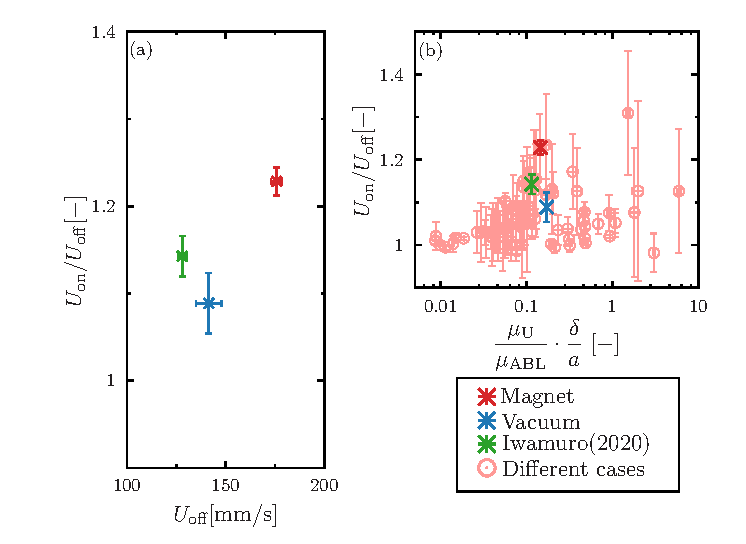
\includegraphics[width=1\textwidth]{./X-Appendix/magnet_vacuum/magnet_vacuum_cal.eps}
    \caption{Relationship velocity ratio and (a)terminal velocity, (b)viscosity ratio.}
    \label{fig:falling-Udiff}
\end{figure}

% \subsection{落下開始時のオーバーシュートへの影響}
% \label{sec:dis-de}

% 今回,球を把持する手法を,電磁石を用いて把持する方法から真空ポンプを用いて把持する方法に変化させた.この時,落下開始時0-0.3sにおける落下速度のオーバーシュートが,先行研究\cite{ref:8,ref:9}より小さくなった.落下開始時のオーバーシュートは弾性による影響によって生じる\cite{ref:12}.以下で,オーバーシュートが見られなくなった原因を,物質の流動性を表す$De$数より考える.$De$数が大きくなると,弾性的傾向が強くなり,$De$数が小さくなると,粘性的流動を表す.

% $De$数は下記の様に緩和時間$\lambda$,代表時間$T$の比で表される.
% \begin{equation}
%     De = \frac{\lambda}{T} .
%     \label{eq:De}
% \end{equation}
% 代表時間$T$に関して,超音波照射を行っていない場合の球の落下条件においても考えるため,
% \begin{equation}
%     T = \frac{a}{U} ,
%     \label{eq:T}
% \end{equation}
% となる.ここで,球の落下速度$U$,球の半径$a$である.また,緩和時間$\lambda$は,粘度$\mu$,貯蔵弾性率$G'$を用いて,
% \begin{equation}
%     \lambda \approx \frac{\mu}{G'} ,
%     \label{eq:lamda}
% \end{equation}
% と見積もられる.緩和時間は変形の経過時間において,粘弾性流体が流体的挙動を示すか,固体的挙動を示すかの指標である\cite{ref:sakanishi}.粘度$\mu$に関して,落下球によるせん断領域における粘度となるため,式(\ref{eq:muU})の$\mu_\text{U}$を用いる.

% これら式(\ref{eq:De}),(\ref{eq:T}),(\ref{eq:lamda}),(\ref{eq:muU})より,$De$数は,
% \begin{equation}
%     De \sim \frac{k}{G'} {\left(\frac{U}{a}\right)}^n ,
%     \label{eq:De2}
% \end{equation}
% となり,粘度定数$k$,貯蔵弾性率$G'$,落下速度$U$,球の半径$a$によって見積もられる.

% 貯蔵弾性率$G'$に関して,Fig.\ref{fig:PAA-elast}にて示した応力との関係性の結果を用いる.ここで応力$\tau$は,落下球によって生じた応力$\tau_\text{U}$を用いる.

% Fig. \ref{fig:iwamuro-fall}に先行研究であるIwamuro \textit{et al}.\cite{ref:8}の球径ごとの実験結果を示す.Fig.\ref{fig:falling-A}, \ref{fig:iwamuro-fall}それぞれの結果より,ピーク速度$U_{peak}$と終端速度$U_{ave}$を算出した.続いて,式(\ref{eq:tau-cal})を用いて,それぞれの速度における応力$\tau_{peak}$,$\tau_{ave}$の算出を行った.これら算出結果と先行研究の計測結果Fig.\ref{fig:iwamuro-G}より,貯蔵弾性率$G'$も求めた.これらの結果を,Table \ref{table:iwamuro}に示す.

% また,式(\ref{eq:muU})を用いて,ピーク速度/終端速度それぞれの粘度$\mu_{peak}$,$\mu_\text{U}$を概算した.これらの粘度を式(\ref{eq:lamda})に代入し,それぞれの緩和時間$\lambda_{peak}$,$\lambda_{ave}$の算出を行った.そして,それらの緩和時間より,式(\ref{eq:De})を用いて,それぞれの$De$数,$De_{peak}$,$De_{ave}$を求めた.これらの結果を,Table \ref{table:iwamuro2}に示す.

% Table \ref{table:iwamuro2}より,ピーク速度より求めた$De_{peak}$と,終端速度より求めた$De_{ave}$において,大きな差異が見られないことが分かった.以降,$De_{peak}$に関してのみ議論を行う.$De_{peak}$に関して,落下速度のオーバーシュート$U_{peak}/U_{ave}$との関係をFig.\ref{fig:De-overshoot}に示す.横軸は$De$数,縦軸は落下速度のオーバーシュート$U_{peak}/U_{ave}$である.この図より,$De$数とオーバーシュートには正の相関があり,$De$数が増加するとオーバーシュートも大きくなることが分かった.

% \begin{table}[H]
%     \caption{Peak speed $U_{peak}$/ terminal speed $U_{ave}$, stress $\tau$, storage modulus $G'$ Calculation result.}
%     \label{table:iwamuro}
%     \centering
%     \begin{tabular}{ccccccc}
%         \hline
%         \multirow{2}{*}{実験者}  & 球直径[mm] & ピーク速度[mm/s] & 終端速度[mm/s] & \multicolumn{2}{c}{応力[Pa]} & 貯蔵弾性率[Pa]        \\
%                                  & $D=2a$     & $U_{peak}$       & $U_{ave}$      & $\tau_{peak}$                & $\tau_{ave}$   & $G'$ \\
%         \hline \hline
%         \multirow{8}{*}{Iwamuro} & 3          & 10.08            & 9.05           & 14.6                         & 14.2           & 8    \\
%                                  & 4          & 23.2             & 19.4           & 16.5                         & 15.9           & 7    \\
%                                  & 5          & 34.8             & 32.6           & 17.2                         & 17.0           & 6.7  \\
%                                  & 6          & 46.3             & 54.8           & 17.6                         & 18.3           & 6.5  \\
%                                  & 7          & 79.8             & 82             & 19.3                         & 19.4           & 5.5  \\
%                                  & 8          & 130              & 113            & 20.9                         & 20.3           & 5    \\
%                                  & 9          & 193              & 133            & 22.3                         & 20.5           & 4    \\
%                                  & 10         & 256              & 168            & 23.2                         & 21.2           & 3.5  \\
%         \hline \hline
%         Niwa                     & 10         & 148              & 144            & 18.9                         & 18.7           & 6    \\
%         \hline
%     \end{tabular}
% \end{table}
% \begin{table}[H]
%     \caption{Viscosity $\mu$, Relaxation time $\lambda$, number of $De$ Calculation result.}
%     \label{table:iwamuro2}
%     \centering
%     \begin{tabular}{ccccccccc}
%         \hline
%         \multirow{2}{*}{実験者}  & 球直径     & \multicolumn{2}{c}{粘度[Pa$\cdot$s]} & \multicolumn{2}{c}{緩和時間[s]} & \multicolumn{2}{c}{$De$数[-]}                                              \\
%                                  & $D=2a$[mm] & $\mu_{peak}$                         & $\mu_{ave}$                     & $\lambda_{peak}$              & $\lambda_{ave}$ & $De_{peak}$ & $De_{ave}$ \\
%         \hline \hline
%         \multirow{8}{*}{Iwamuro} & 3          & 2.17                                 & 2.36                            & 0.27                          & 0.29            & 1.82        & 1.78       \\
%                                  & 4          & 1.42                                 & 1.63                            & 0.20                          & 0.23            & 2.36        & 2.26       \\
%                                  & 5          & 1.24                                 & 1.30                            & 0.18                          & 0.19            & 2.57        & 2.53       \\
%                                  & 6          & 1.14                                 & 1.00                            & 0.18                          & 0.15            & 2.71        & 2.82       \\
%                                  & 7          & 0.85                                 & 0.83                            & 0.15                          & 0.15            & 3.51        & 3.53       \\
%                                  & 8          & 0.64                                 & 0.72                            & 0.13                          & 0.14            & 4.19        & 4.05       \\
%                                  & 9          & 0.52                                 & 0.69                            & 0.13                          & 0.17            & 5.58        & 5.12       \\
%                                  & 10         & 0.45                                 & 0.63                            & 0.13                          & 0.18            & 6.64        & 6.03       \\
%         \hline \hline
%         Niwa                     & 10         & 0.64                                 & 0.65                            & 0.11                          & 0.11            & 3.15        & 3.12       \\
%         \hline
%     \end{tabular}
% \end{table}

% \begin{figure}[H]
%     \begin{center}
%         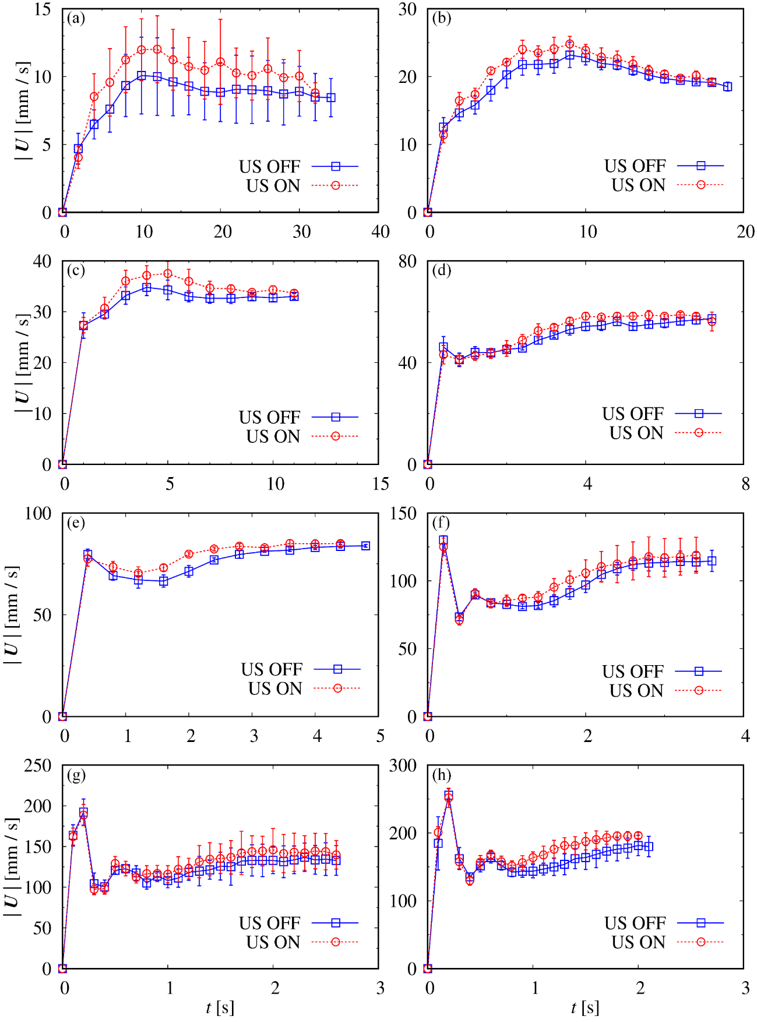
\includegraphics[width=13cm,clip]{X-Appendix/over_shoot/iwamuro-fall.png}
%         \caption{Speed of a falling sphere in diameter of (a) 3 mm, (b) 4 mm, (c) 5 mm, (d) 6 mm, (e) 7 mm, (f) 8 mm, (g) 9 mm, (h) 10 mm in 1.0 wt.\% PAA solution with ultrasound fixed frequency at 27.4 kHz and $\Delta \bar{P} \approx$ 180 kPa\cite{ref:8}.}
%         \label{fig:iwamuro-fall}
%     \end{center}
% \end{figure}

% \begin{figure}[H]
%     \begin{center}
%         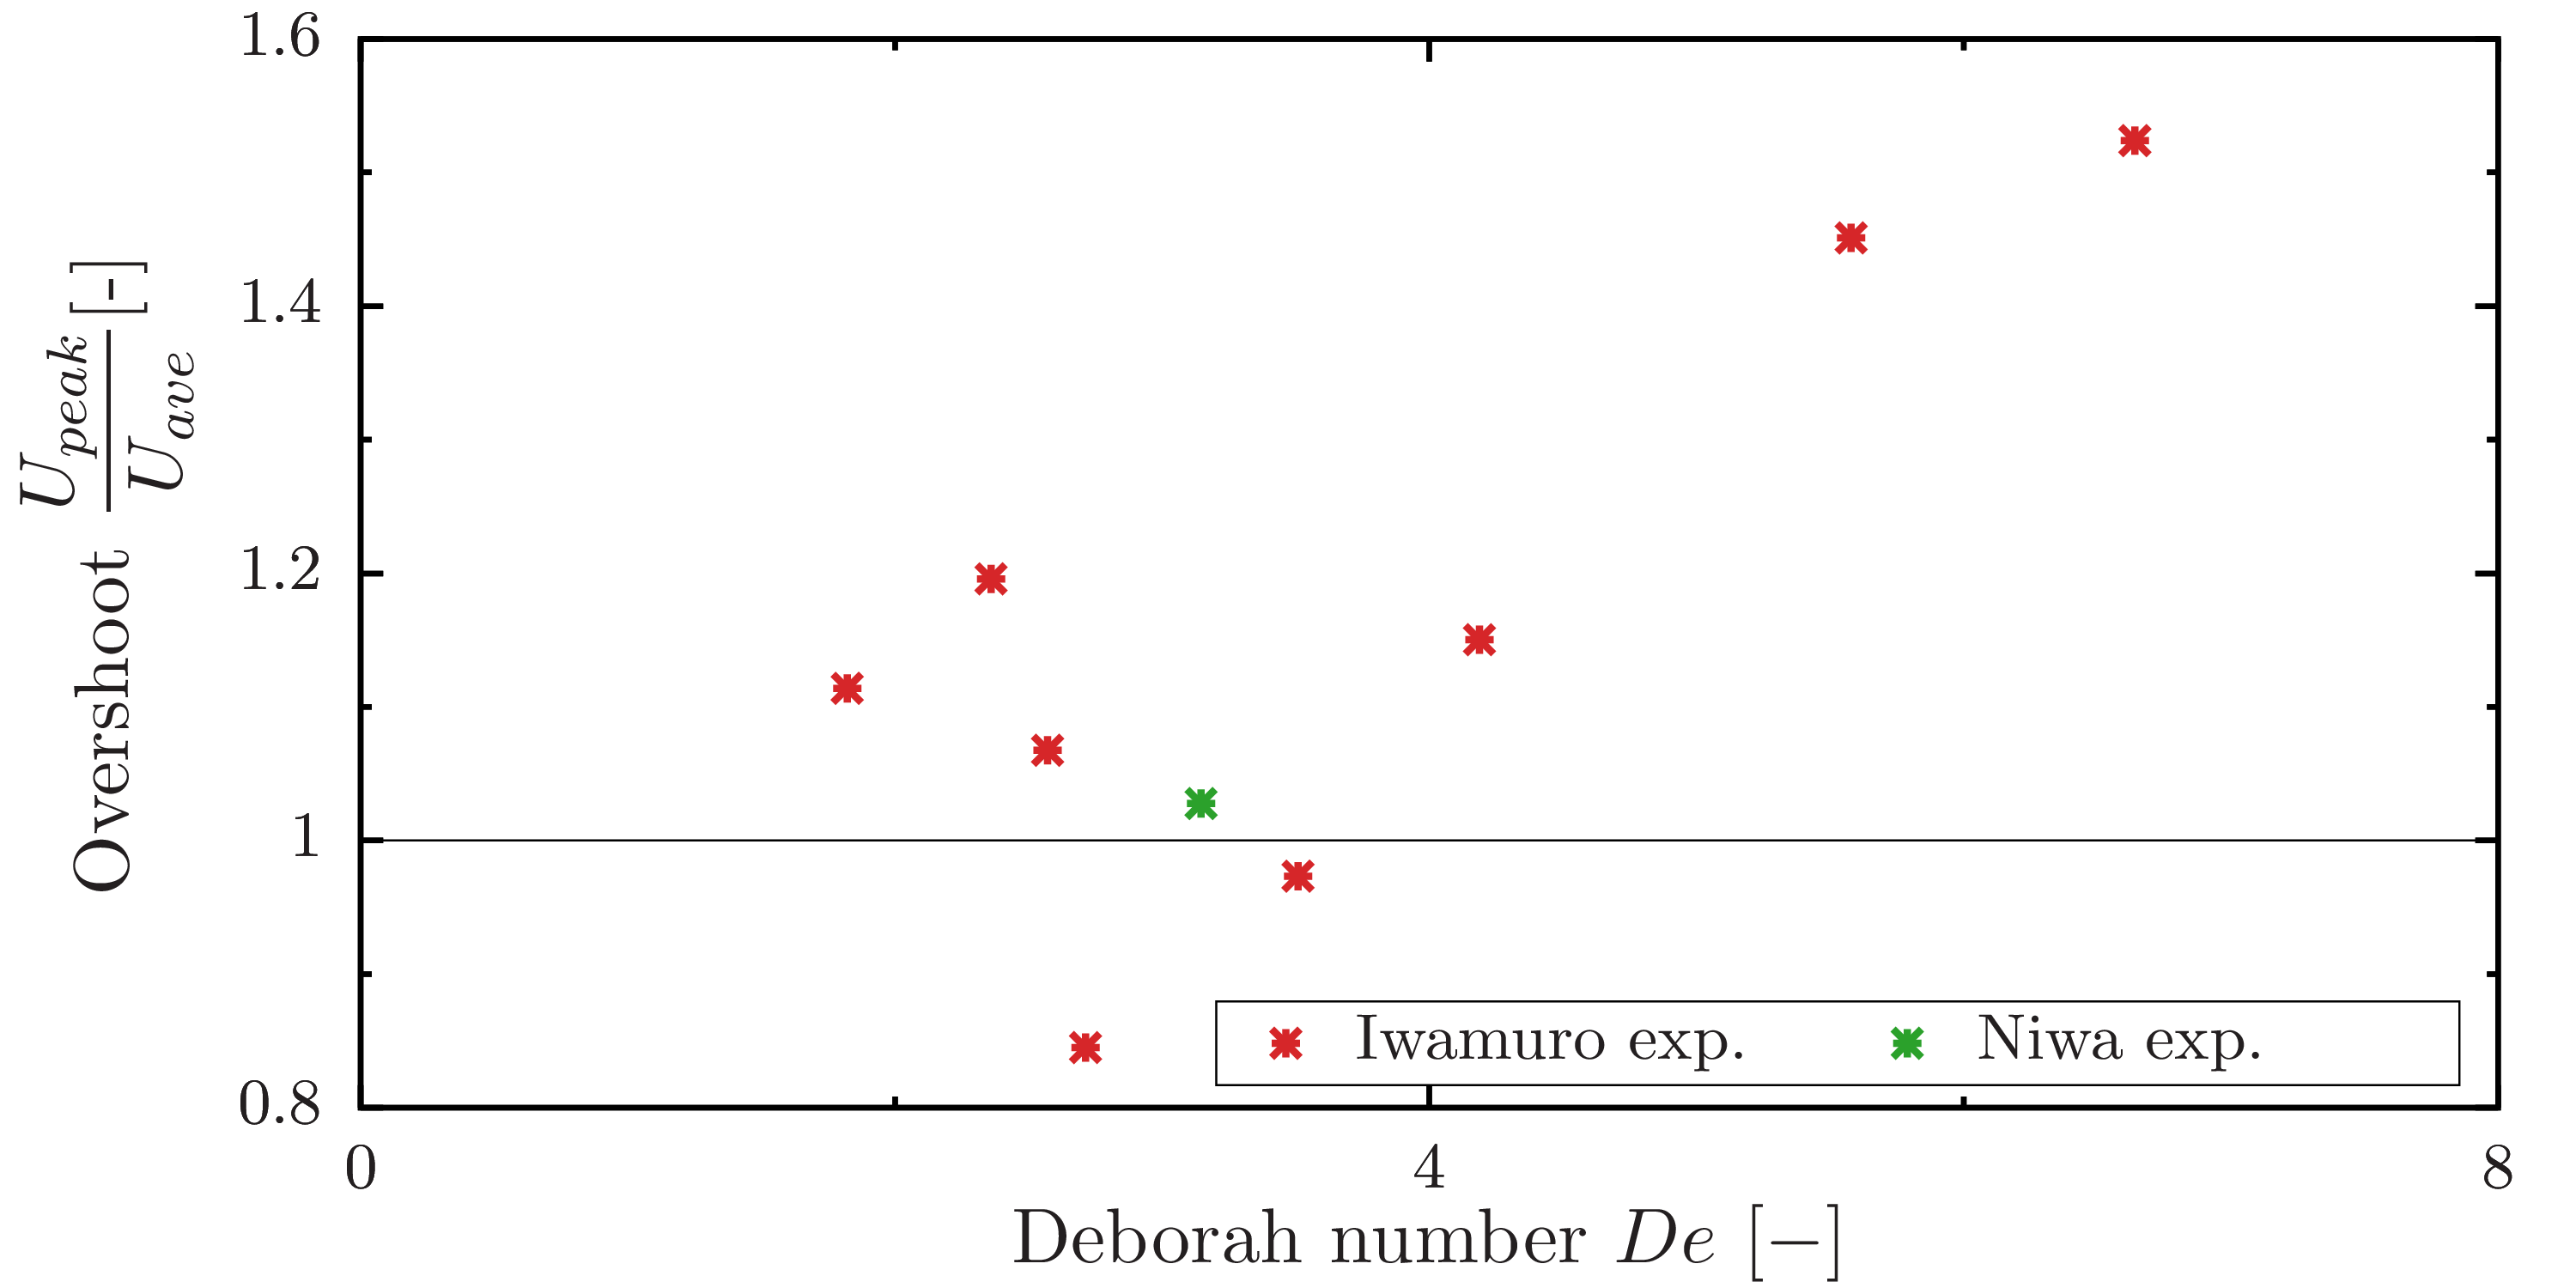
\includegraphics[width=15cm,clip]{5-Results/De-overshoot.png}
%         \caption{Relationship between overshoot $U_{peak}/U_{ave}$ and Deborah number $De$ for falling spheres.}
%         \label{fig:De-overshoot}
%     \end{center}
% \end{figure}

\section{初速による影響に関して}
\label{sec:interval-velocity}
\ref{sec:reexp}章にて,実験装置の改良によってピーク速度が減少し,オーバーシュートが小さくなったことを示した.本節において,電磁石を用いて把持した場合,ピーク速度が大きくなった理由に関して考察を行う.電磁石を用いて球を把持した場合,電磁石へ落下方向に力を与えて落下を開始させている.この時,微小ではあるが落下開始時に初速が存在する.一方で真空ポンプを用いて球を把持した場合,吸着パッドを大気圧にすると球は落下する.この場合,球に力が加わらないため,初速は存在しない.このように初速の有無がオーバーシュートの変化に大きく関与していると考えられる.

初速の有無が与える影響に関して調査するため,真空ポンプを用いて球中心が液面より高さ$H=$5mmとなる地点で把持し,そこから球を落下させた.その結果をFig.\ref{fig:h-5}に示す.縦軸は落下速度,横軸は初速ありの場合は液面に球中心が入ったときを0s,初速なしの場合は落下開始時刻を0sとした時刻である.この条件において,初速は313mm/sとなる.ピーク速度は440mm/sとなり,初速を超えて加速した.これは初速と重力による加速が,粘性抵抗や浮力よりも大きく,弾性は遅れて発生するため,初速を超えて加速したと考えられる.よって,電磁石を用いて球を把持した場合は初速による影響がオーバーシュートとして現れるが,真空ポンプを用いて球を把持した場合は初速が非常に小さいためその影響を受けないということが分かった.

\begin{figure}[H]
    \begin{center}
        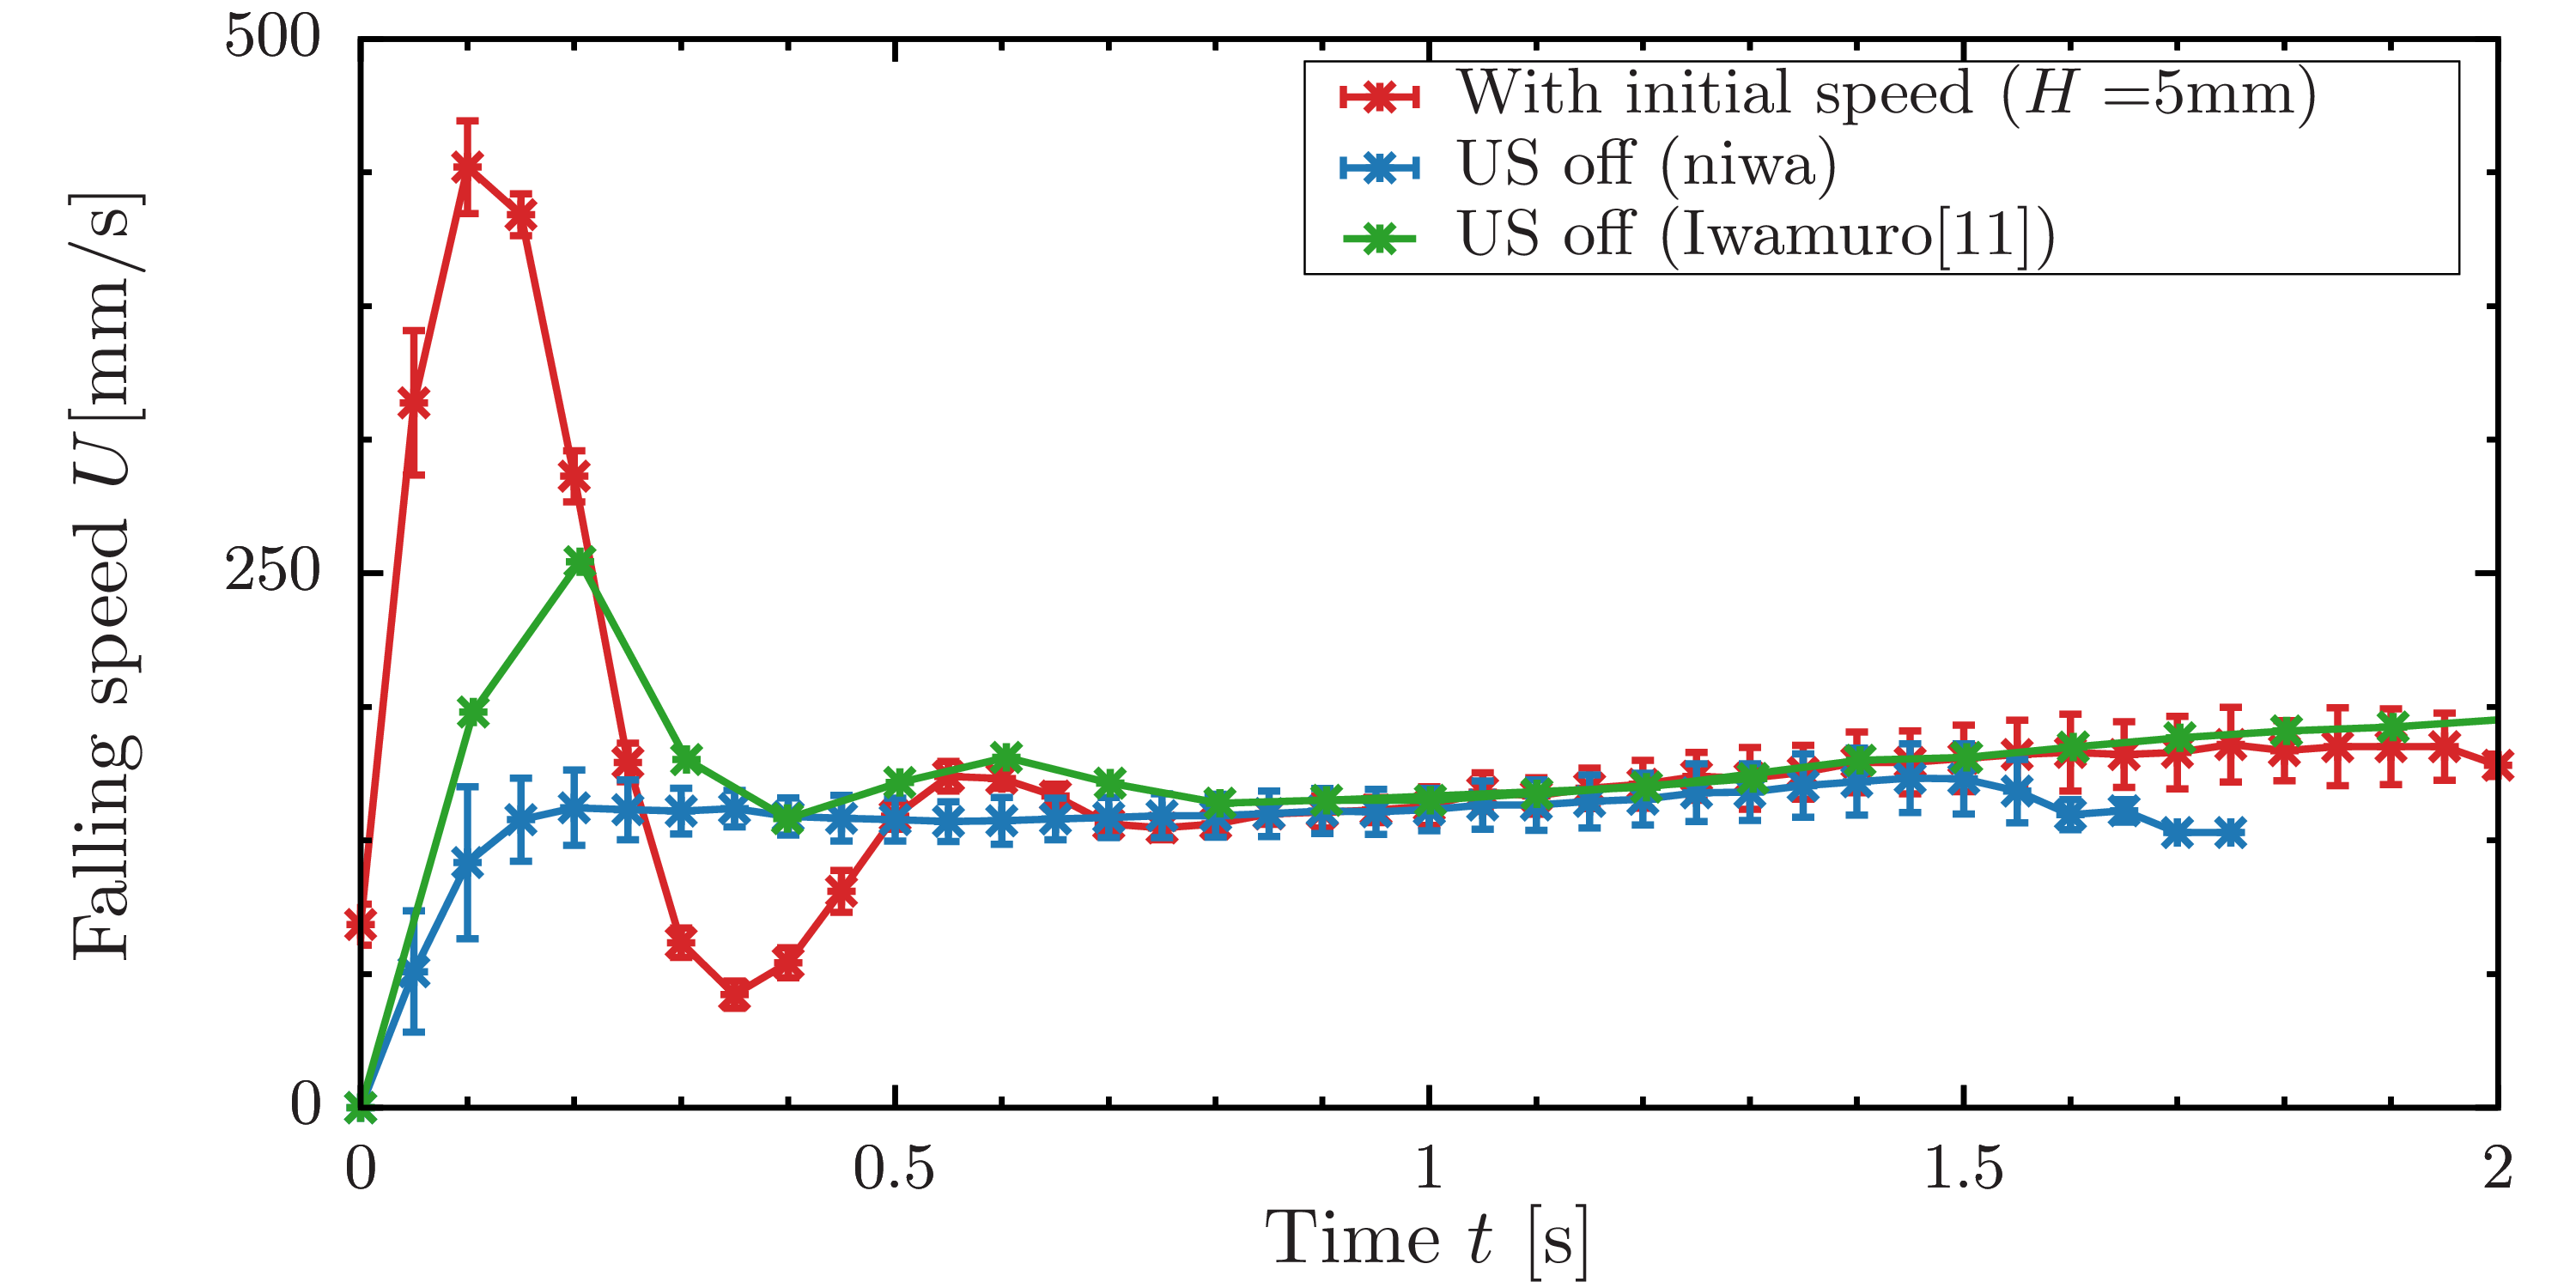
\includegraphics[width=15cm,clip]{X-Appendix/h-5.png}
        \caption{Falling speed of a sphere in 1.0wt.\% PAA solution falling with initial speed.}
        \label{fig:h-5}
    \end{center}
\end{figure}
	\clearpage
	\section{落下間隔変化における擬塑性流体の経時変化}

Fig. \ref{fig:falling-5-2}, \ref{fig:falling-10-2}, \ref{fig:falling-20-2}に落下間隔を5分, 10分, 20分と変化させた実験における落下速度の経時変化を示す.縦軸は落下速度,横軸は落下開始時からの経過時間である.溶液の作成後,7日後と60日後に落下速度の計測を行った.溶液作成7日後のが,60日後よりもより超音波による高速化の影響を受けた.また,落下速度は時間経過とともに早くなった.これは溶液の経時変化によって粘度が小さく溶液が変化したためと考えられる.

\begin{figure}[ht]
    \centering
    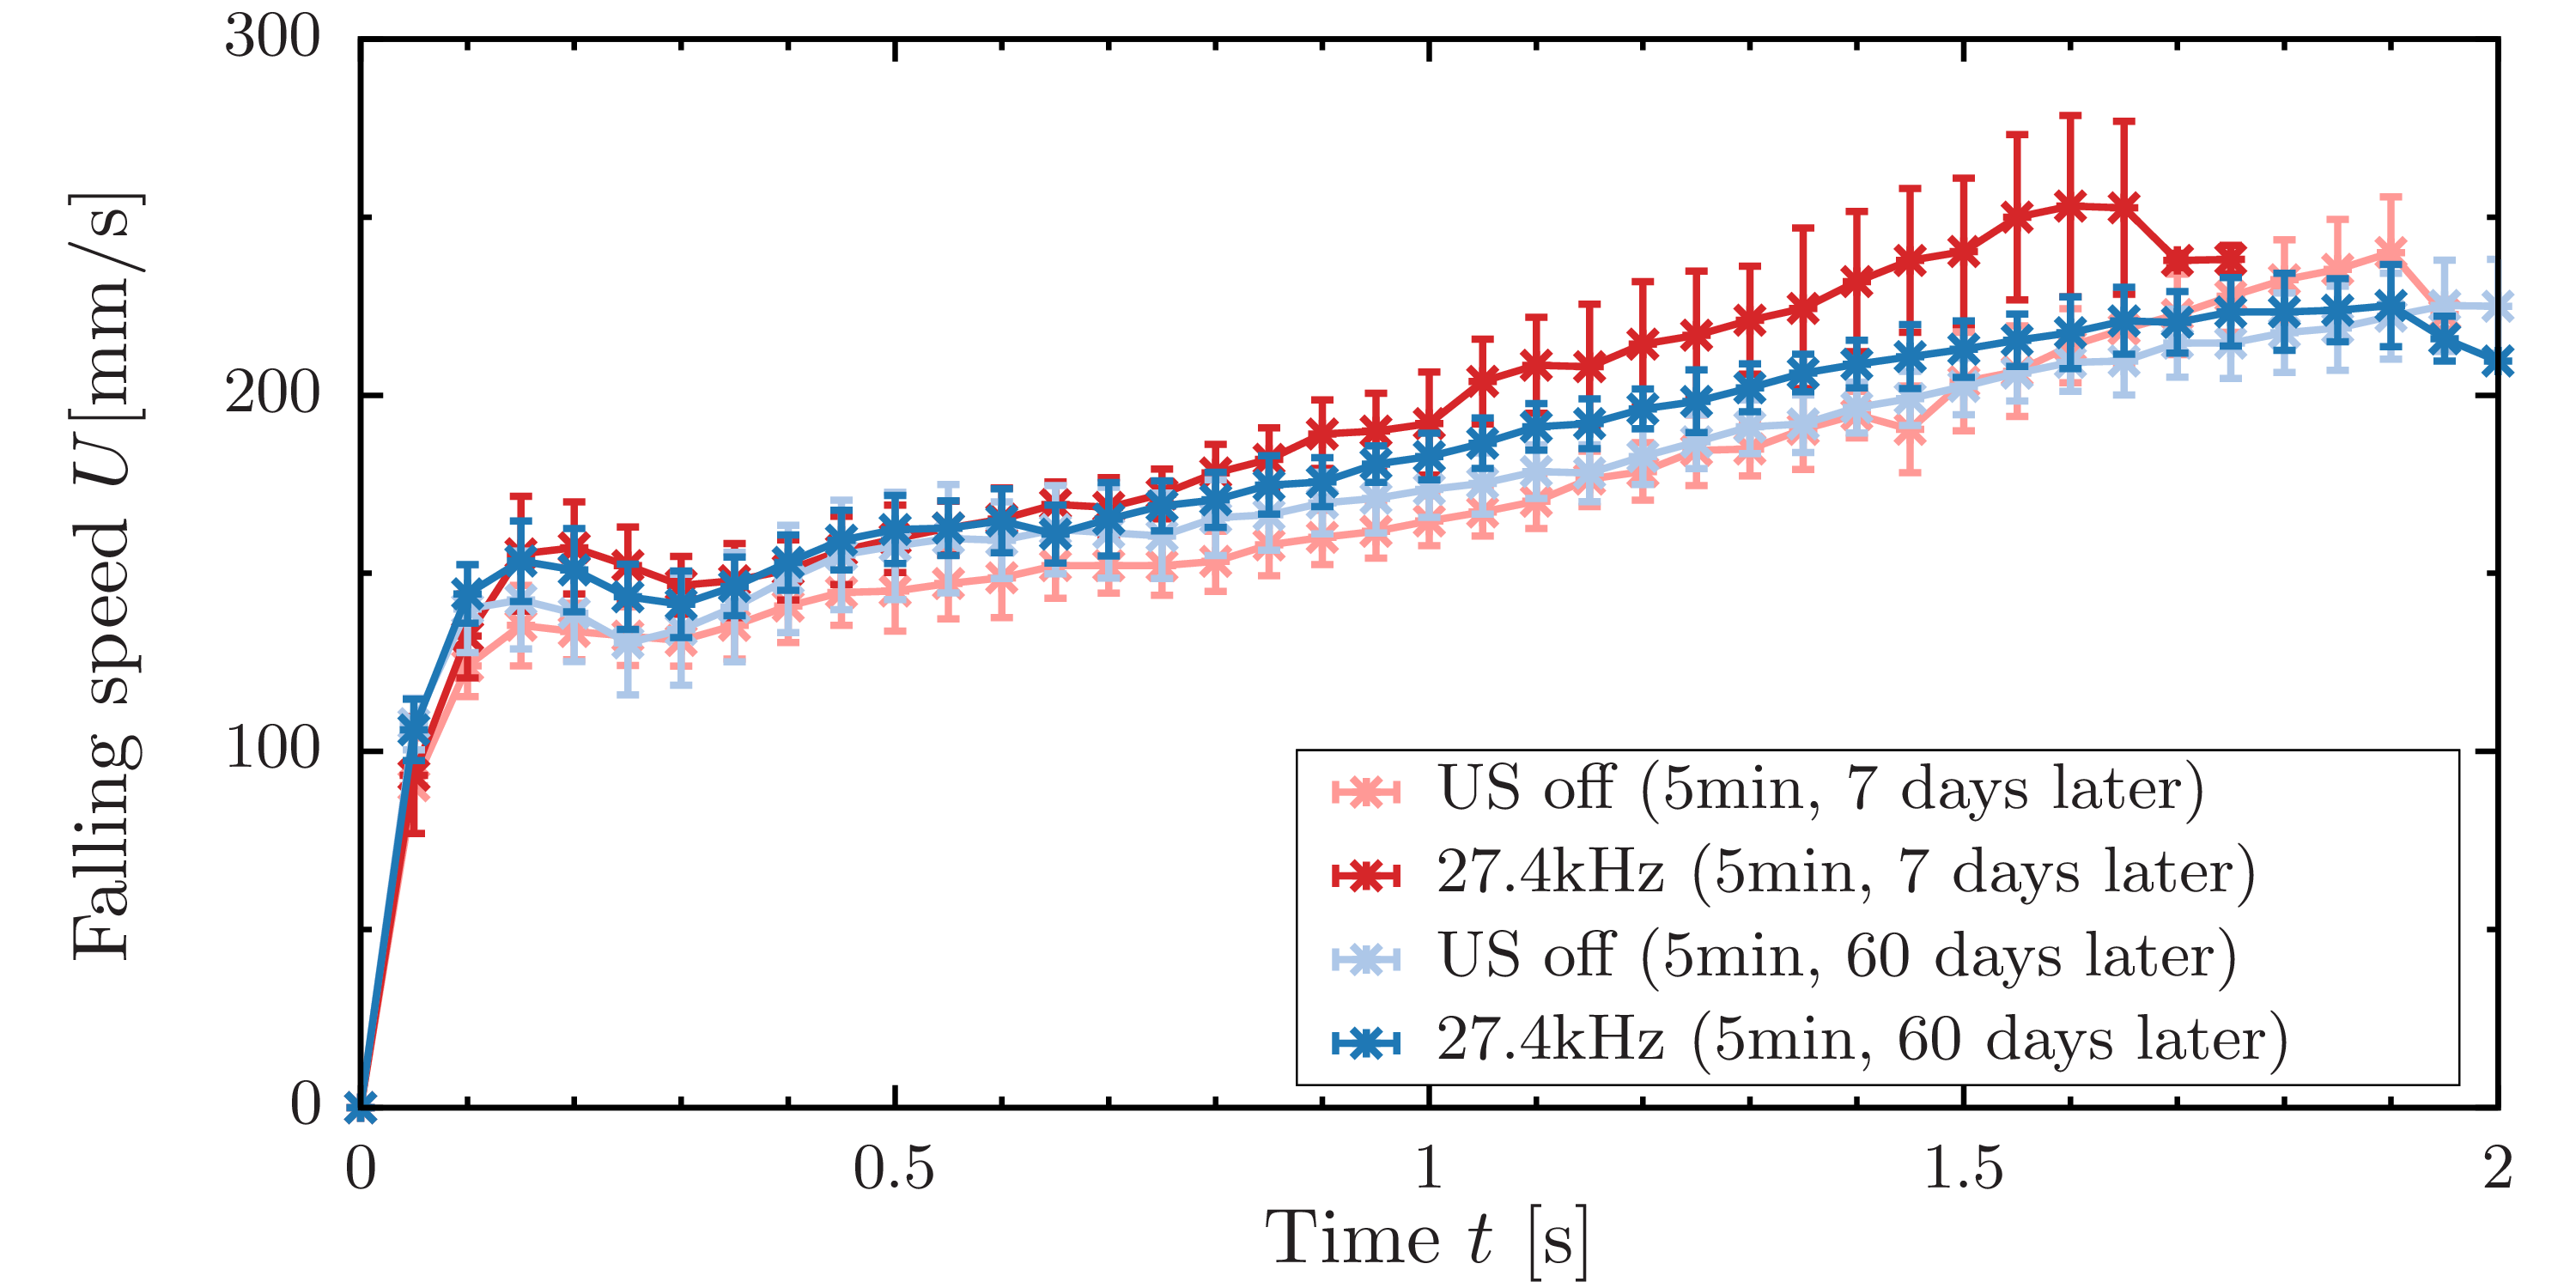
\includegraphics[width=11cm,clip]{X-Appendix/5.png}
    \caption{Falling velocity of a sphere in 1wt.\%PAA solution with and without ultrasound irradiationin tank B. Comparison of changes over time. (Interval 5 min.)}
    \label{fig:falling-5-2}
\end{figure}
\begin{figure}[ht]
    \centering
    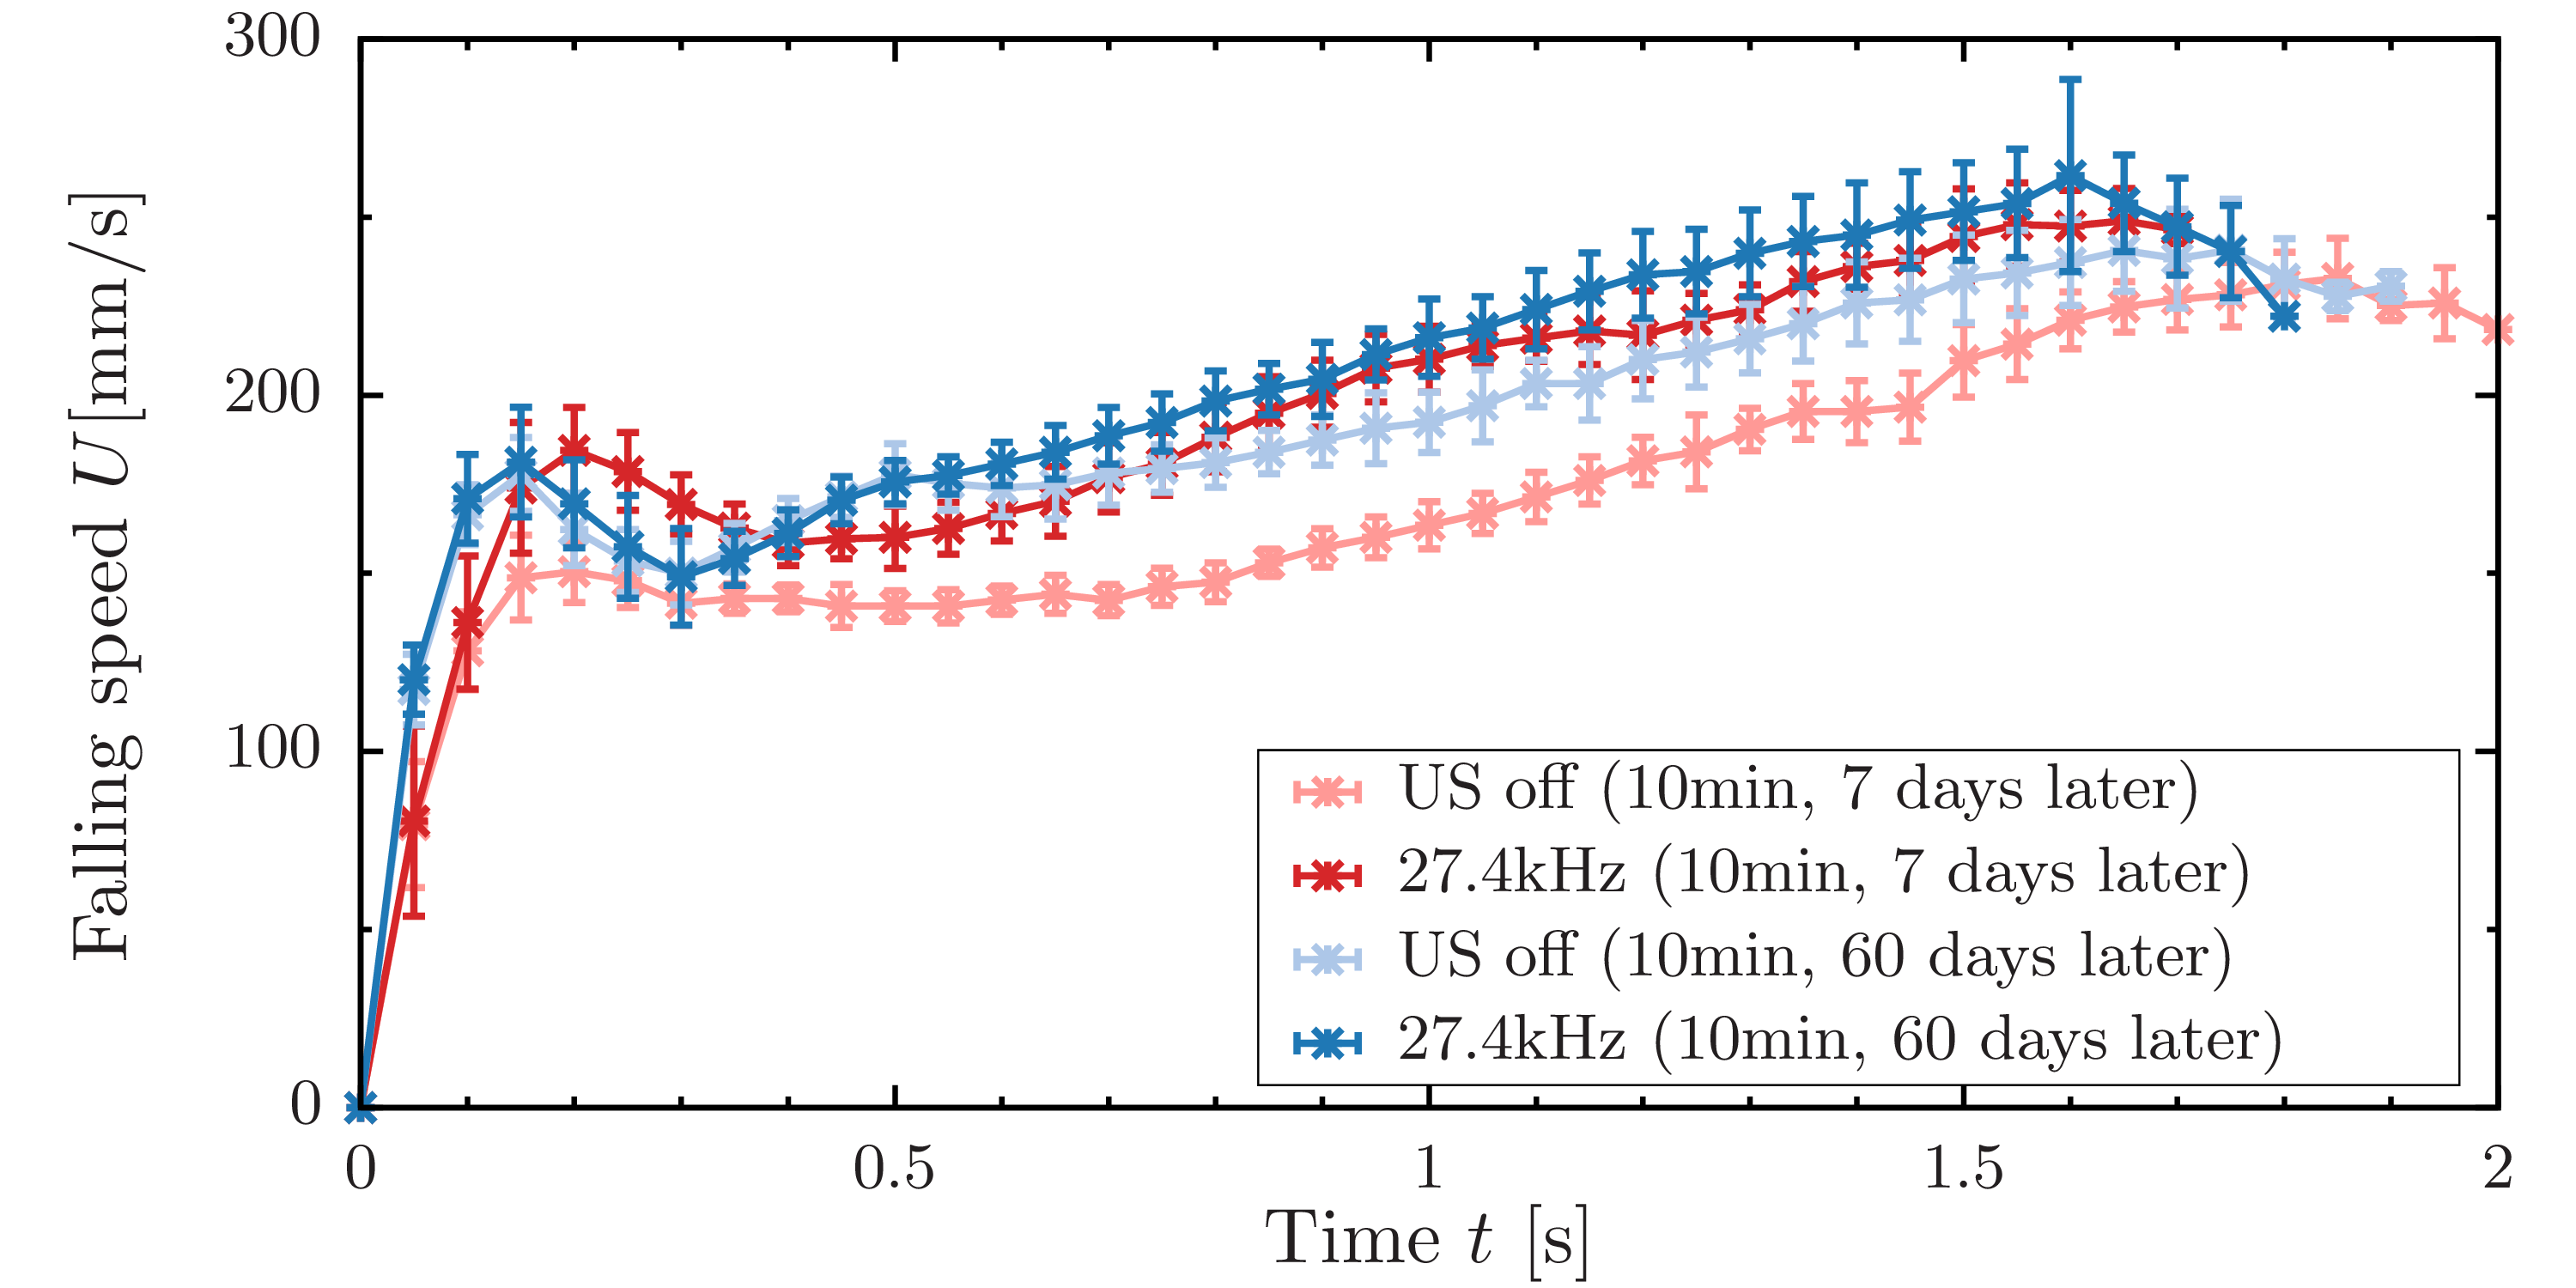
\includegraphics[width=11cm,clip]{X-Appendix/10.png}
    \caption{Falling velocity of a sphere in 1wt.\%PAA solution with and without ultrasound irradiationin tank B. Comparison of changes over time. (Interval 10 min.)}
    \label{fig:falling-10-2}
\end{figure}
\begin{figure}[ht]
    \centering
    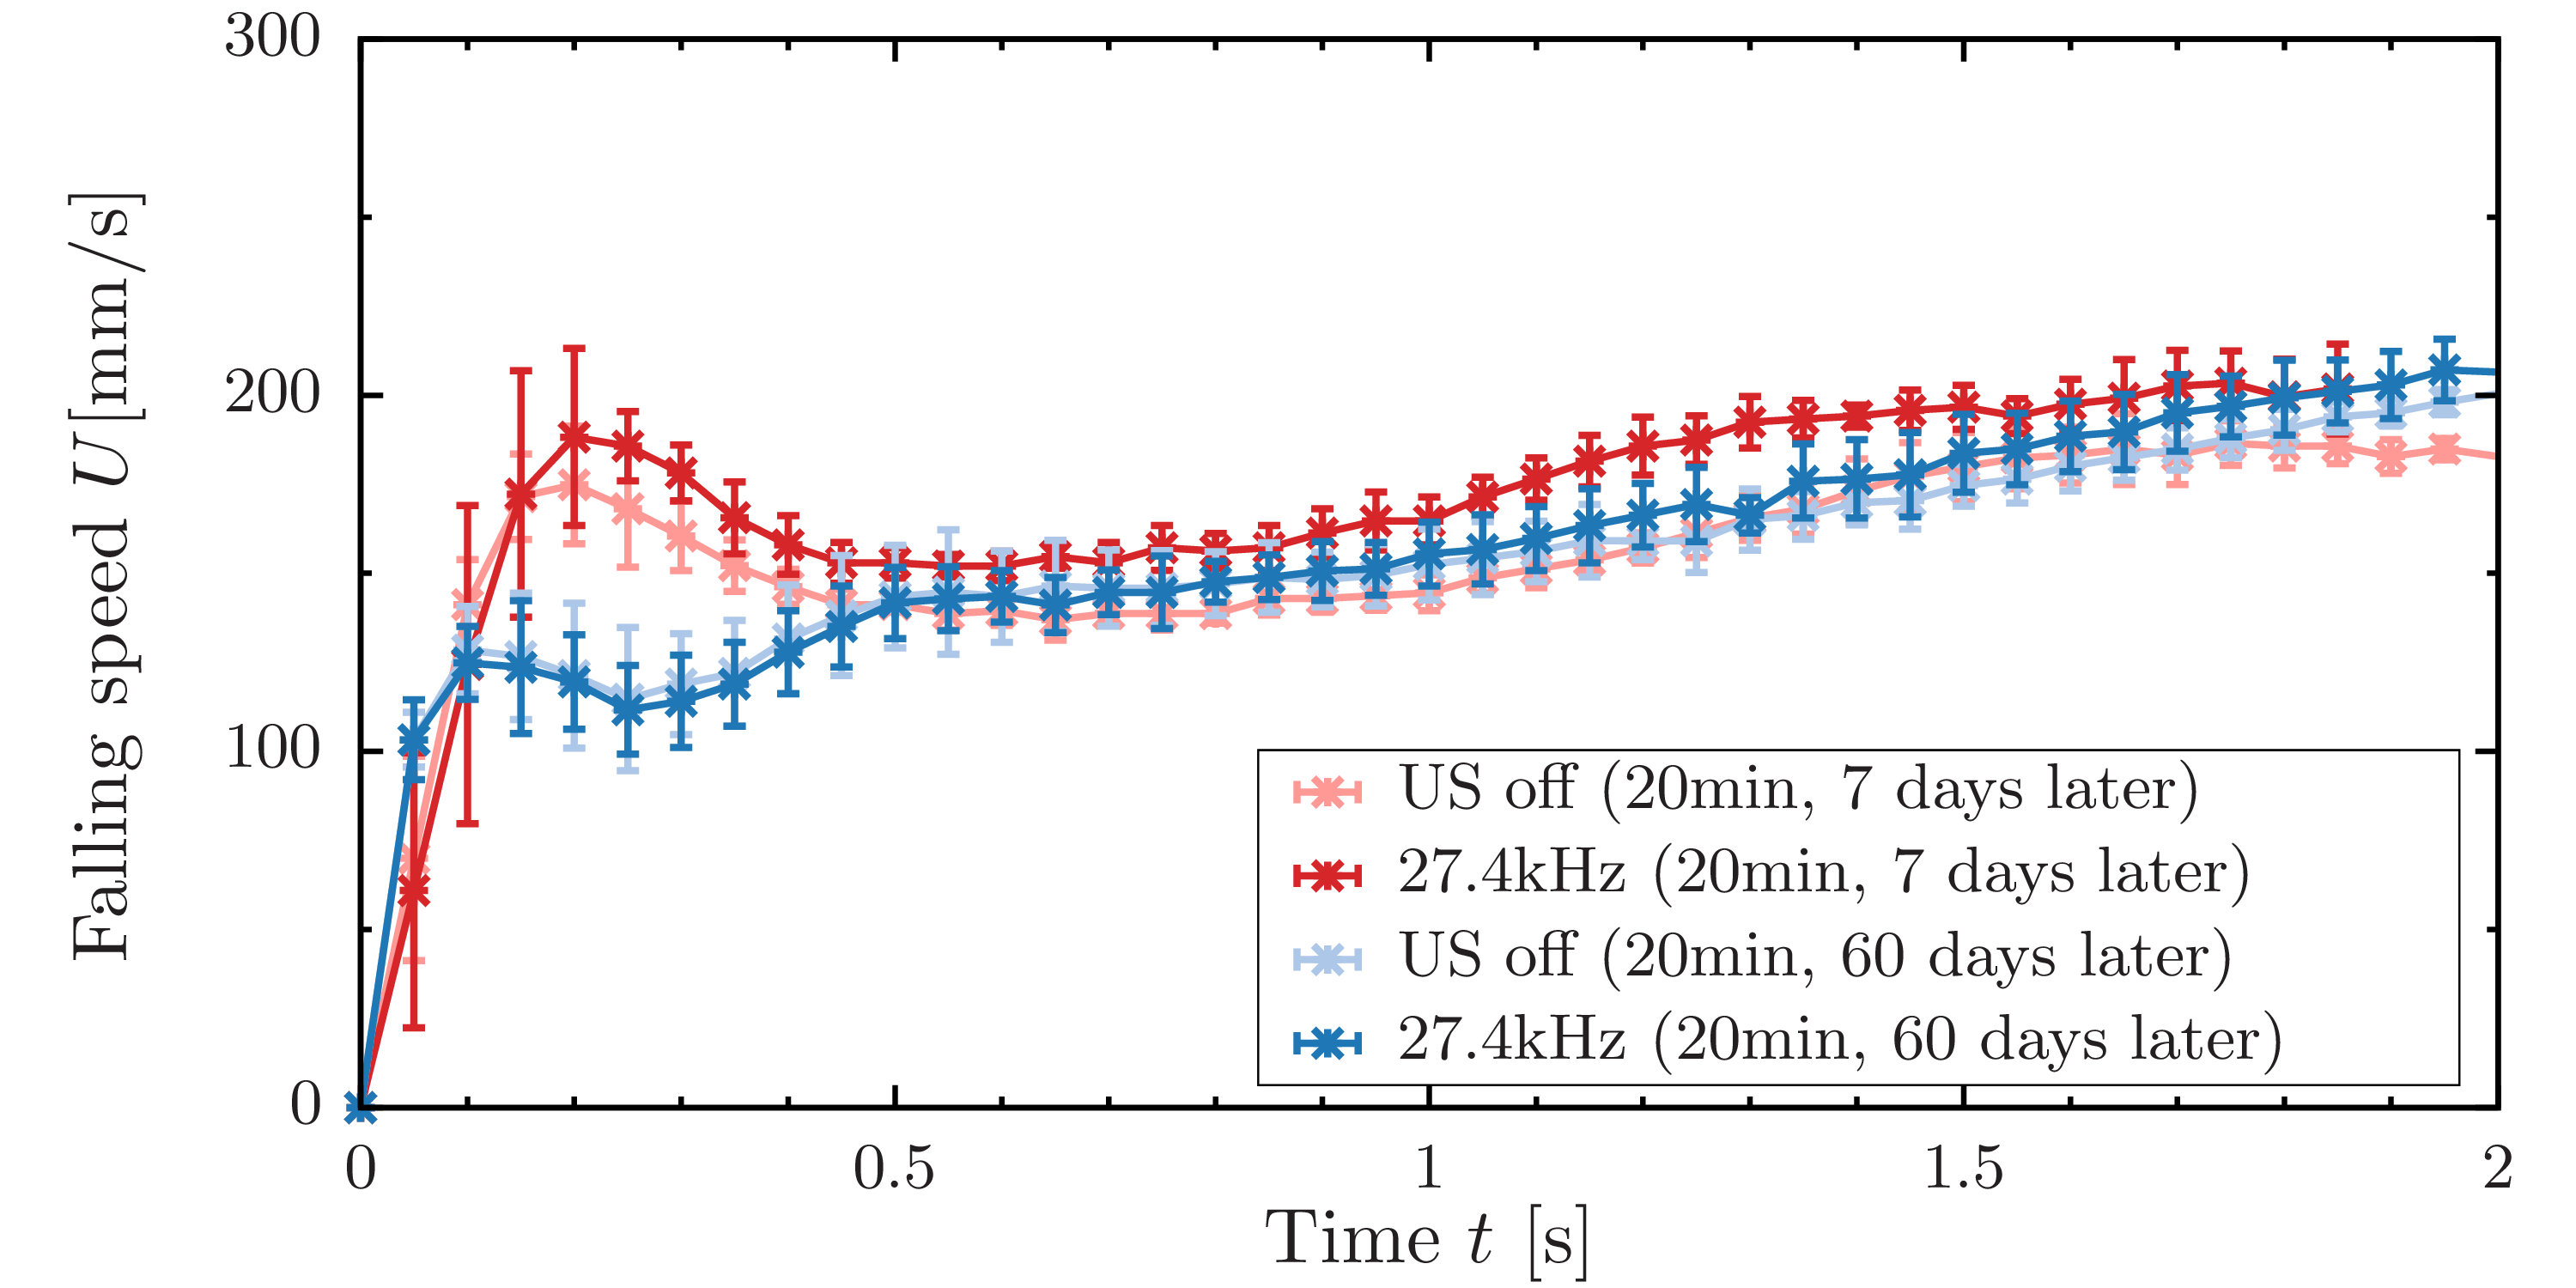
\includegraphics[width=11cm,clip]{X-Appendix/20.png}
    \caption{Falling velocity of a sphere in 1wt.\%PAA solution with and without ultrasound irradiationin tank B. Comparison of changes over time. (Interval 20 min.)}
    \label{fig:falling-20-2}
\end{figure}

	\clearpage
	\section{溶液作製精度に関して}

溶液の作製精度の確認を行うため,0.95,1.00,1.05wt.\%のPAA溶液を作製した.それぞれの擬塑性流体に直径10mmの鋼球を落下させ,終端速度の変化,超音波照射による影響の変化の確認を行った.

\subsection{溶液の粘性特性に関して}
それぞれの溶液の特性を確認するため,粘度計を用いて粘度計測を行った.粘度計測を行った結果をFig.\ref{fig:95-105}に示す.比較のため,先行研究である岩室\cite{ref:8}とShiratori \it{et al}.\cite{ref:9}の計測結果も合わせて示す.濃度が薄いと粘度は低く,濃度が高いと粘度は高くなった.

\begin{figure}[ht]
    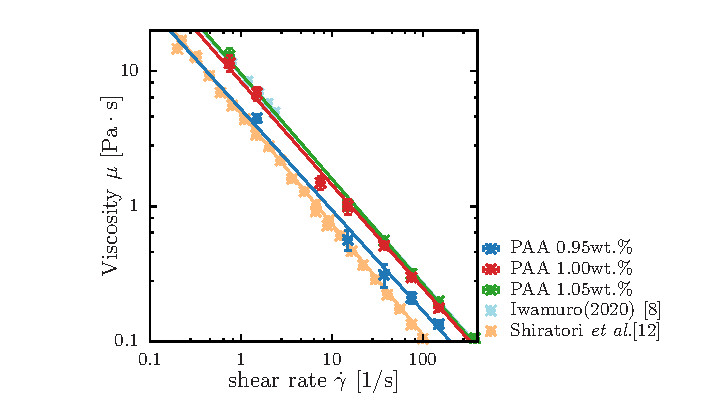
\includegraphics[width=0.8\textwidth]{X-Appendix/concentration/viscosity/viscosity.eps}
    \caption{Viscosity versus shear rate for PAA0.95,1.00,1.05wt.\%.}
    \label{fig:95-105}
\end{figure}

\subsection{溶液の作製精度による高速化への影響に関して}

ぞれぞれの質量濃度のPAA溶液に対し,落下球実験を行った.落下させた球は,鋼製の直径10mmの球である.

\subsection{溶液の作製精度と終端速度の関係}

実験装置の改良により終端速度に差異がみられた.終端速度の差異に関して考察を行う.式(\ref{eq:UT})より,Power-Law modelにおける,$k$,$n$のパラメータより終端速度を見積もることができる.

Table \ref{table:power-law}の結果より,式(\ref{eq:UT})を用いて直径10mmの球におけるIwamuro\cite{ref:8}の終端速度$U_I$を基準とした終端速度の比$U_T/U_{I}$を求めた.その結果を,Table \ref{table:UT}に示す.これより,今回の粘度特性において,Iwamuro\cite{ref:8}と比較して終端速度が1.09倍速くなることが分かった.Fig.\ref{fig:falling-A}において,Iwamuro\cite{ref:8}と比較して1.125倍,終端速度が速かった.一方で,0.95,1.05wt.\%それぞれのPAA溶液の粘度特性における終端速度比と比較しても実験結果と一番近いのは,1wt.\%の場合である.よって,溶液の濃度精度は1wt.\%±0.05wt.\%以内であり,溶液の作製誤差によって落下速度に差が生じたと考えられる.

\begin{table}[h]
    \centering
    \caption{Each parameter($k$,$n$) and terminal speed ratio in the power-law model for each experimental result.}
    \label{table:UT}
    \begin{tabular}{c|c|c|c} \hline
                                                     & $k$  & $n$  & $U_T/U_{I}$ \\ \hline \hline
        Present Value(1.05wt.\%)                     & 9.56 & 0.23 & 0.93        \\
        Present Value(1wt.\%)                        & 8.37 & 0.24 & 1.09        \\
        Present Value(0.95wt.\%)                     & 5.22 & 0.25 & 3.91        \\
        岩室\cite{ref:8}                             & 9.4  & 0.23 & 1           \\
        Shiratori \textit{et al}.(2016)\cite{ref:10} & 5.9  & 0.25 & 2.99        \\ \hline
    \end{tabular}
\end{table}


	\clearpage
	\section{落下間隔変化における高速化への寄与}
球の落下間隔を変化させると、PAA溶液の粘性弾性回復に対して影響を与えると考えられる.これらの落下速度,高速化への影響を調査するため,落下間隔を変化させた実験を行った.

\subsection{落下実験結果}

落下間隔を5分,10分,20分と変化し,球を落下させた解析した結果をFig.\ref{fig:falling-interval}に示す.縦軸は落下速度,横軸は落下開始時からの経過時間である.それぞれの場合において,超音波照射による落下球の高速化は見られた.

なお,落下間隔10分の結果に関して,比較のため先行研究であるIwamuro\cite{ref:9}における実験結果もあわせて示す.

しかし,Iwamuro\cite{ref:9}と比較し,落下開始時の加速におけるオーバーシュートが今回は見られなかった.また,Iwamuro\cite{ref:9}においては落下速度は落下開始から0.8s以降,定常状態となっている.本実験において同条件である落下間隔10分において,超音波照射なしの場合,落下開始から0.2-0.7s間のみ,一定速度で落下し以降は加速した.オーバーシュートの有無は先述の装置改良における実験結果においても見られたため,実験手法の変化によるためだと考えられる.終端速度への到達の有無だが,擬塑性流体の粘弾性回復がIwamuro\cite{ref:9}と比較して十分に行われていないと考えられる.これは,落下間隔20分の条件において,Iwamuro\cite{ref:9}と同様の終端速度に達しているため,落下間隔10分では回復しきれなかった粘弾性が回復しきったためだと考えられる.粘弾性の回復時間が異なることに関しては,落下間隔をより細かく変化させ調査する必要があると考えられる.

\begin{figure}[ht]
    \centering
    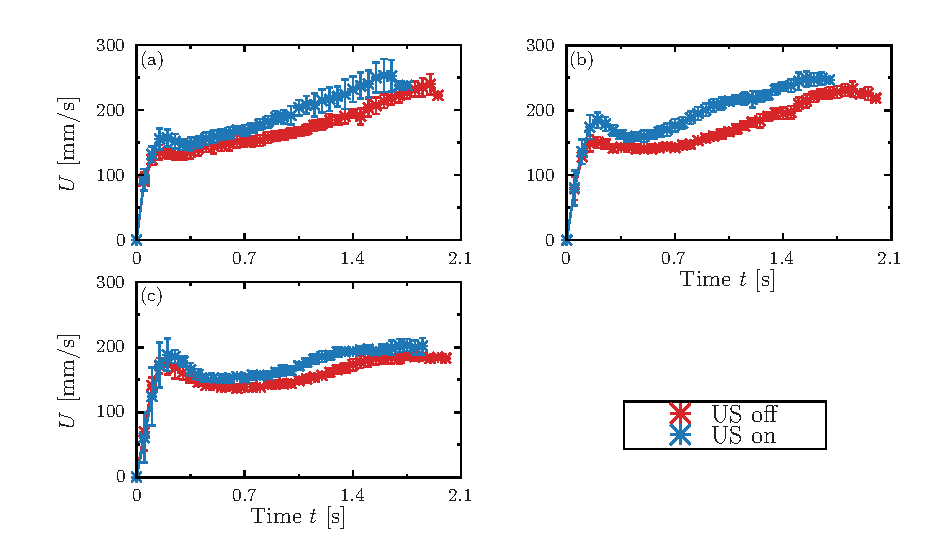
\includegraphics[width=1\textwidth]{./X-Appendix/interval/interval.eps}
    \caption{Falling speed of a sphere in 1wt.\%PAA solution with and without ultrasound irradiation for the interval (a)5min, (b)10min, (c)20min.)}
    \label{fig:falling-interval}
\end{figure}

\clearpage

\subsection{超音波照射による高速化}

球の落下間隔を5分,10分,20分と変化させた.その結果をFig.\ref{fig:interval-change}に示す.なお,縦軸は落下速度[mm/s],横軸は落下開始時からの経過時間[s]である.全ての条件において超音波照射に伴う高速化は見られた.また落下速度は,落下間隔10分,5分,20分の順で速かった.この結果を元に,超音波照射時の球の落下速度$U_{on}$と超音波照射なしの球の落下速度$U_{off}$として,速度比$U_{on}/U_{off}$を求めた.その結果をFig.\ref{fig:speed-diff}に示す.ここで縦軸は速度比[-],横軸は落下間隔時間[min]である.この結果より,落下速度と同様に,落下間隔10分,5分,20分の順で超音波照射による高速化が見られた.これに関して,超音波照射による高速化のメカニズムより考える.

今回,落下間隔を変化させたが,音響圧$\Delta P$,水溶液密度$\rho_1$,音速$c$,周波数$f$はすべて同一であった.よって,$k,n$ の2つがパラメータとして考えられる.Iwamuro\cite{ref:9}における擬塑性流体の経時変化や濃度変化における粘性特性の変化\cite{ref:Rahimi2007},\cite{ref:Agi2018} より,$n$よりも$k$の方がパラメータとして大きく作用することが分かる.よって,$k$のみをパラメータとして扱うと,速度比$U_{ABL}/U_0$は,$k^\frac{n}{n+1}$によって変化することが分かる.ここで,$n=0.24$とすると,$\delta \propto k^{0.19}$となり,境界層厚さは粘度定数に対して単調増加する.また,式(\ref{eq:power-law})より,$k$が増加すると粘度$\mu$は大きくなり,式(\ref{eq:UT})より落下速度は遅くなることも分かる.ゆえに,粘度が大きくなると落下速度が遅くなり,境界層厚さが厚くなる.

今回,落下間隔を変化させた実験結果をFig.\ref{fig:interval-change}に示す.縦軸は落下速度,横軸は落下開始時刻からの経過時間である.この図に示される様に,超音波照射なしでの落下速度は落下間隔10分,5分,20分の順で速かった.これは,落下間隔の変化で流体の粘弾性特性が変化したためだと考えられる.式(\ref{eq:UT})より,落下間隔10分よりも20分の方のが$k$が大きくなり,粘性が大きくなったと考えられる.超音波照射による落下速度を超音波照射なしにおける速度$U_{OFF}$で規格化した落下間隔ごとの結果をFig.\ref{fig:speed-diff}に示す.超音波照射による高速化も,超音波照射なしの落下速度と同様の順で大きくなった.

Iwamuro\cite{ref:8}において,音響境界層内の粘度とその厚さが超音波照射による高速化の要因と示されていた.今回の実験結果において,音響境界層内粘度および厚さの影響(式(\ref{eq:Udiff}))をFig.\ref{fig:speed-diff-iwamuro}に示す.縦軸は超音波照射ありの場合の終端速度$U_{ON}$を,超音波照射なしの場合の終端速度$U_{OFF}$で規格化したものである.横軸は,$\mu_U$を音響境界層内の粘度$\mu_{ABL}$で規格化し,球半径$a$で規格化し音響境界層厚さ$\delta$を乗じたものである.この図に,本実験の結果だけではなくIwamuro\cite{ref:8}の結果も示す.図において,今回の落下間隔を変化させた実験結果は,単調減少となっている.一方でIwamuro\cite{ref:8}の結果と合わせると,誤差バーの範囲内に存在している.音響境界層内の粘度とその厚さが超音波照射による高速化の要因と示されていた.落下間隔を変化させた場合においても同様に,音響境界層内の粘度とその厚さが超音波照射による高速化の要因となっていることが分かる.

今回は粘性による影響を考えた.一方,落下開始時のオーバーシュートが落下間隔20分の場合のみ見られ,落下間隔を長くすると弾性による影響を受けることも分かる.このため粘性だけではなく,弾性による影響を考慮する必要があるということが考えられる.これを解明するために,それぞれの落下間隔における貯蔵弾性率の計測等も行う必要があると考えられる.

\begin{figure}[ht]
    \begin{center}
        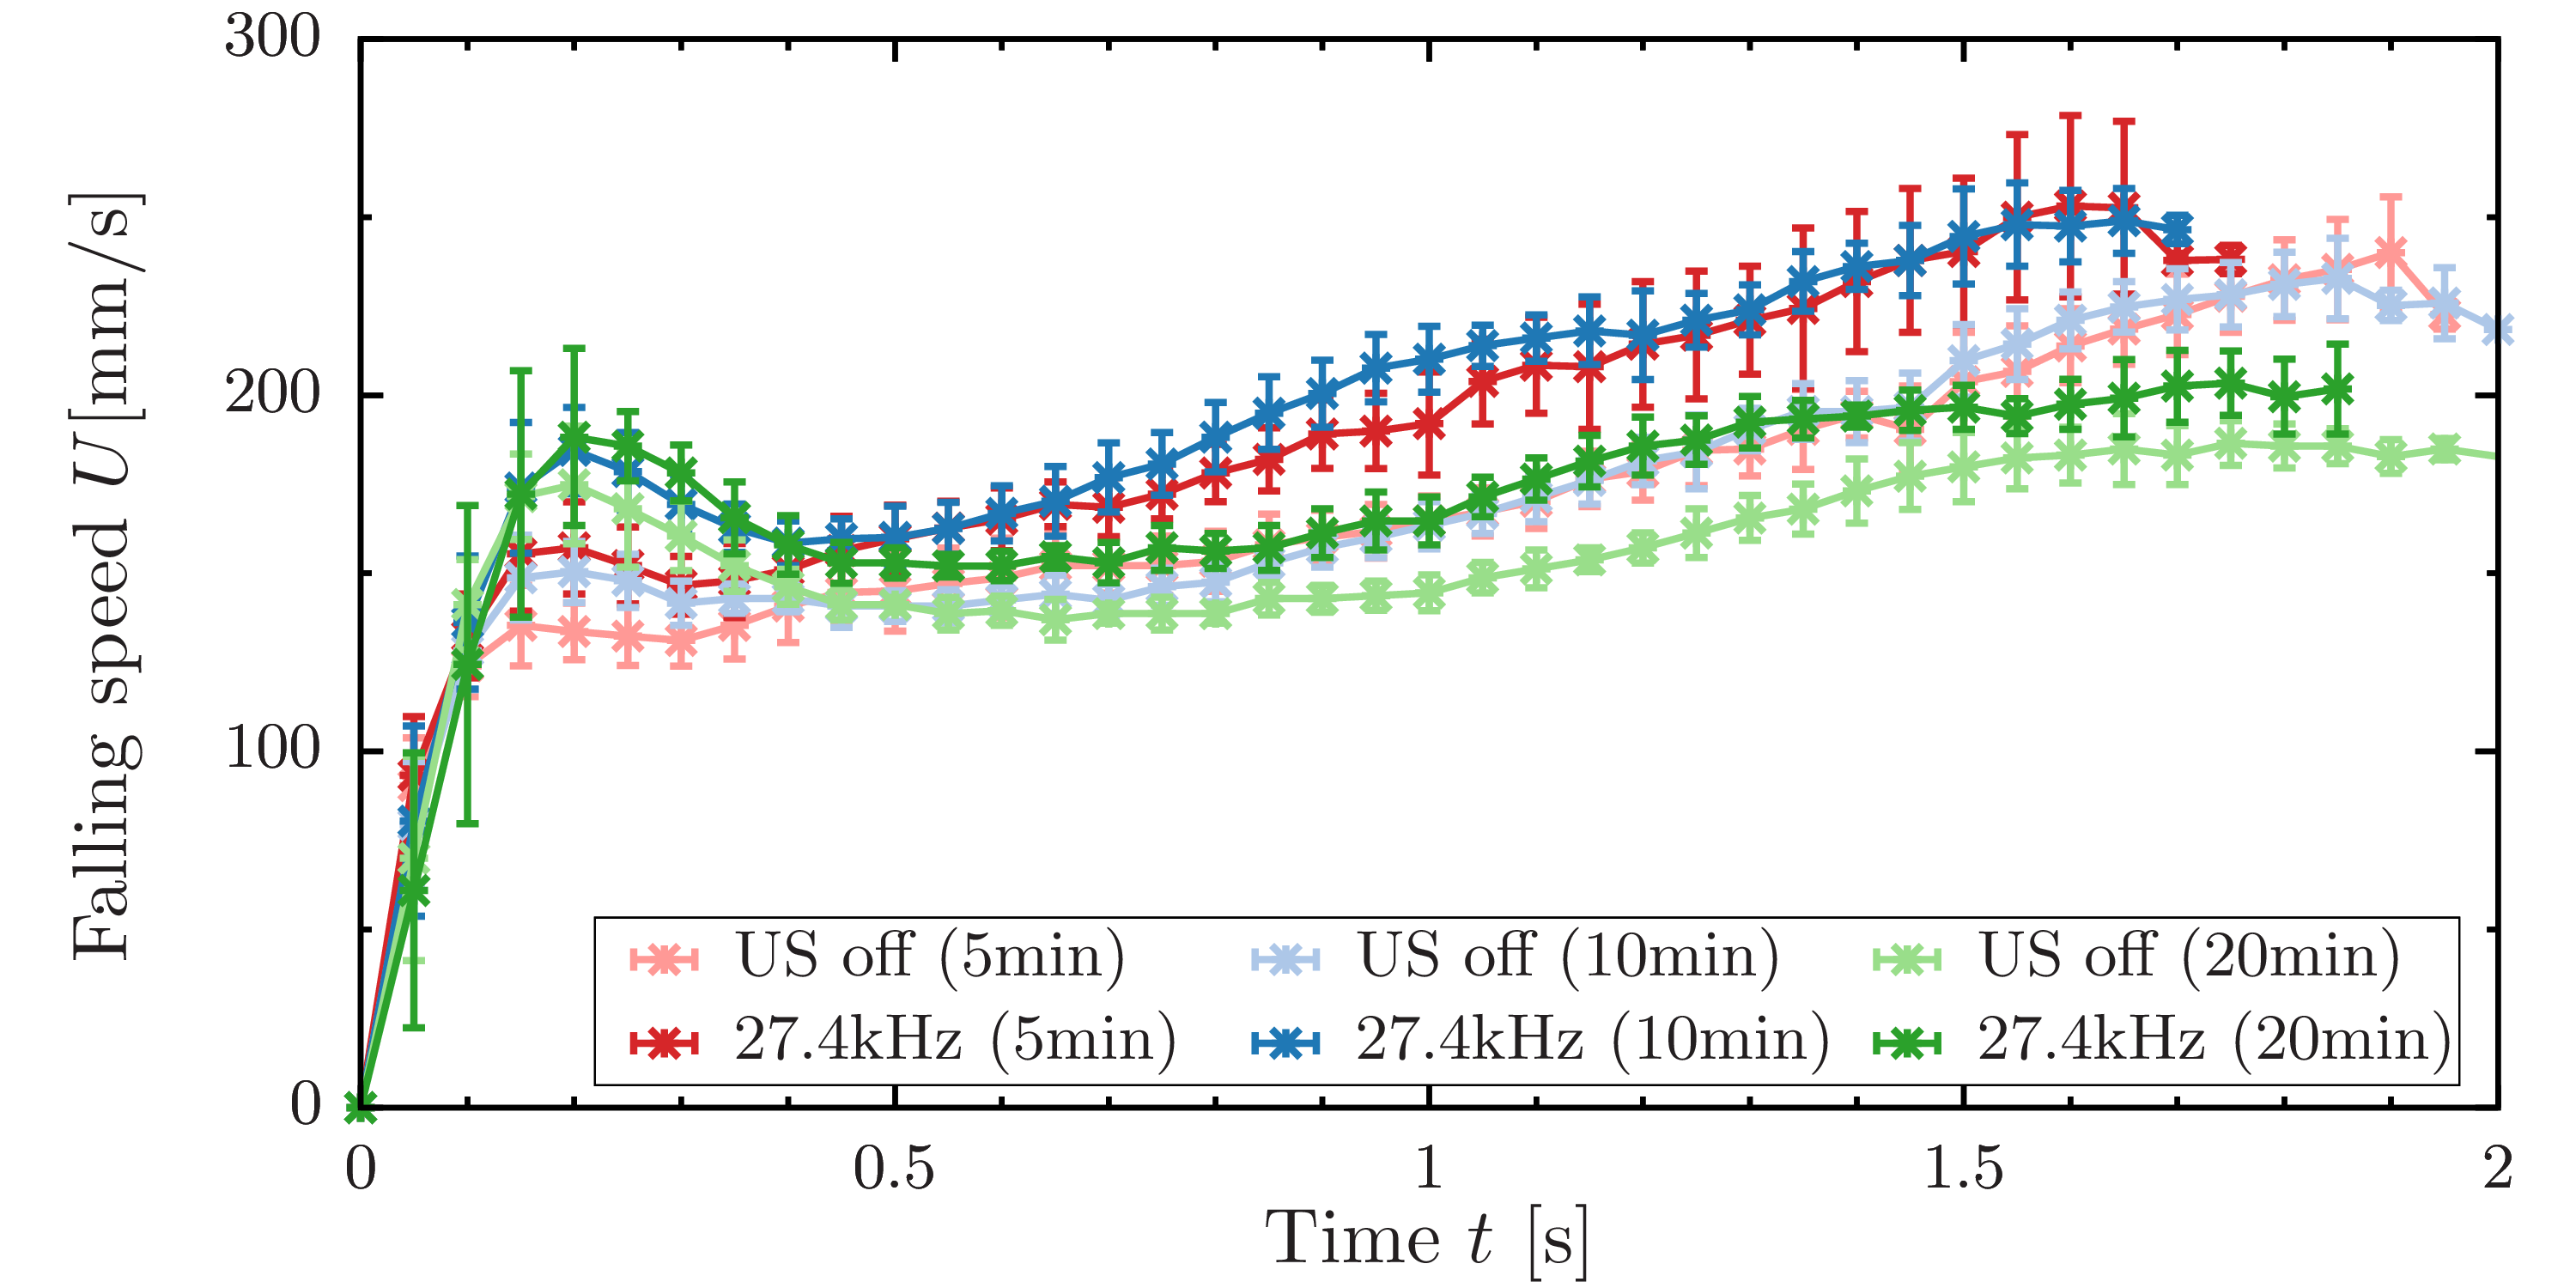
\includegraphics[width=13cm,clip]{5-Results/interval.png}
        \caption{Drop interval change Experimental results.}
        \label{fig:interval-change}
    \end{center}
\end{figure}

\begin{figure}[ht]
    \begin{center}
        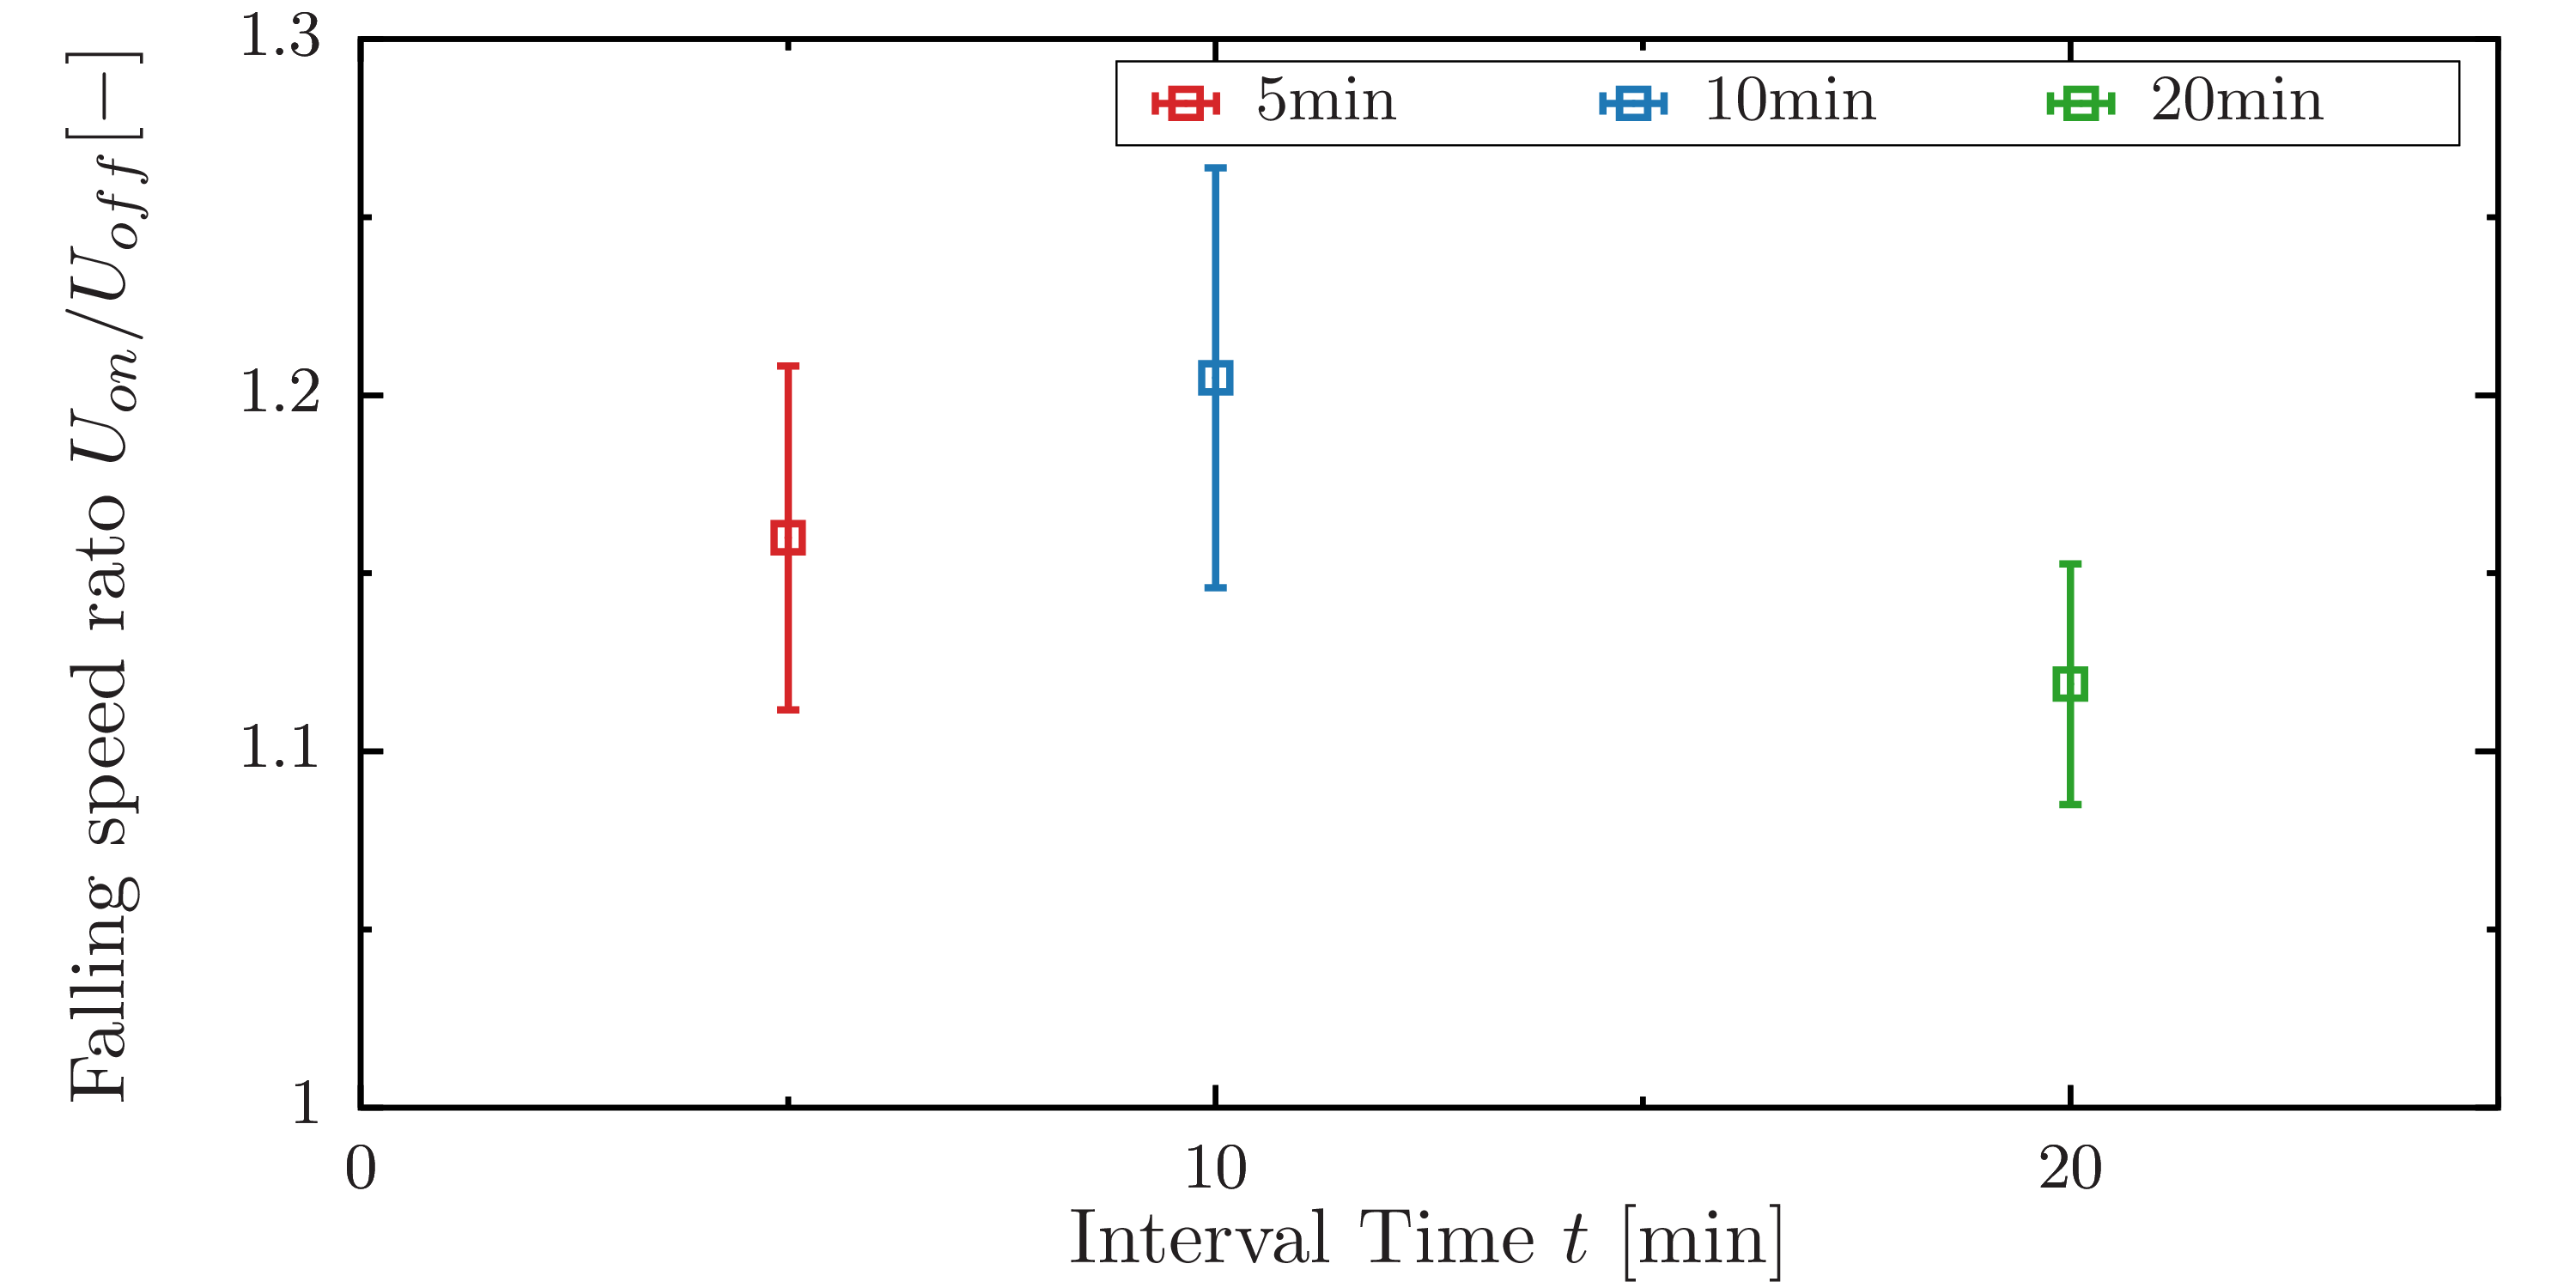
\includegraphics[width=13cm,clip]{5-Results/diff.png}
        \caption{Falling speed ratio due to ultrasound irradiation with change in fall interval.}
        \label{fig:speed-diff}
    \end{center}
\end{figure}

\begin{figure}[ht]
    \begin{center}
        \includegraphics[width=13cm,clip]{5-Results/diff-iwamuro.png}
        \caption{Relationship between viscosity and its thickness in the acoustic boundary layer and speed-up by ultrasound irradiation.}
        \label{fig:speed-diff-iwamuro}
    \end{center}
\end{figure}
	%    \clearpage
	%    \section{落下手法の変化}

本文中における実験は,電磁石ホルダーを用いて鋼球を把持しているため,強磁性の材質の物体のみ把持することができる.
他の物質の物体を把持することのできる爪式ピッキングツールを用いて物体の把持を行い,球の落下試験を行った.
以下にその方法と結果を示す.

\subsection{実験方法}

今回,落下球の把持の方法を変化させただけであるので,実験装置の落下球把持の部分以外は先述の方法と同一である.

\subsubsection{実験装置}

実験装置の模式図をFig.\ref{fig:device2}に示す.先述の通り,電磁石ホルダーではなく,爪式ピックアップツールを用いて球の把持を行った.そして,ピックアップツールの開放を行うことで球を落下させた.それ以外に関しては,本文中の実験装置と同一である.

\begin{figure}[h]
    \centering
    \includegraphics[clip,width=12.0cm]{X-Appendix/device.png}
    \caption{Schematic view of the experimental apparatus.}
    \label{fig:device2}
\end{figure}

\subsection{落下球 実験結果}

1wt.\%PAA溶液中における球の落下速度を解析した結果をFig.\ref{fig:1-1PAA-falling}に示す.縦軸は落下速度,横軸は落下開始時からの経過時間である.先述の電磁石ホルダを用いたFig.\ref{fig:1PAA-falling}とは異なり,超音波照射の有無において落下速度の高速化は見られなかった.一方で,先行研究であるIwamuro {\it et al.}\cite{ref:9}と同様に初めの加速後は減速し一定速度となった.

また,電磁石ホルダを用いた場合と同様に,超音波照射なしの状態における1から5試行目の結果をFig.\ref{fig:1-1PAA-falling1-5}に,6から10試行目の結果をFig.\ref{fig:1-1PAA-falling6-10}に示す.また,超音波照射ありの状態における1から5試行目の結果をFig.\ref{fig:1-1onPAA-falling1-5}に,6から10試行目の結果をFig.\ref{fig:1-1onPAA-falling6-10}に示す.これら試行ごとの結果において,先述のFig.\ref{fig:1PAA-falling1-5}-\ref{fig:1onPAA-falling6-10}の結果とは異なり落下速度のばらつきが非常に小さくなっていた.

\begin{figure}[ht]
    \centering
    \includegraphics[width=12cm,clip]{./X-Appendix/s1.png}
    \caption{Falling velocity of a sphere in 1wt.\%PAA solution with and without ultrasound irradiation.}
    \label{fig:1-1PAA-falling}
    \centering
    \includegraphics[width=12cm,clip]{X-Appendix/s1-0-1-5.png}
    \caption{Falling velocity of the sphere for each trial (\#1 to \#5) in 1wt.\%PAA solution without ultrasonic irradiation.}
    \label{fig:1-1PAA-falling1-5}
\end{figure}
\begin{figure}[ht]
    \centering
    \includegraphics[width=12cm,clip]{X-Appendix/s1-0-6-10.png}
    \caption{Falling velocity of the sphere for each trial (\#6 to \#10) in 1wt.\%PAA solution without ultrasonic irradiation.}
    \label{fig:1-1PAA-falling6-10}
    \centering
    \includegraphics[width=12cm,clip]{X-Appendix/s1-39-1-5.png}
    \caption{Falling velocity of the sphere for each trial (\#1 to \#5) in 1wt.\%PAA solution with ultrasonic irradiation.}
    \label{fig:1-1onPAA-falling1-5}
    \centering
    \includegraphics[width=12cm,clip]{X-Appendix/s1-39-6-10.png}
    \caption{Falling velocity of the sphere for each trial (\#6 to \#10) in 1wt.\%PAA solution with ultrasonic irradiation.}
    \label{fig:1-1onPAA-falling6-10}
\end{figure}
\clearpage
\subsection{考察}

電磁石ホルダを用いた把持方法と爪式ピッキングツールを用いた把持方法では試行ごとの落下速度の時間変化や超音波照射による高速化の有無において変化が見られた.以下に把持方法の変化による影響に関して検討を行う.

まず,電磁石ホルダを使用する場合,落下開始1分前に電源を切り,電磁石ホルダの把持力をゼロにする.しかし,落下させる対象の鋼球や溶液中に把持しているために存在する鋼製棒に磁性が残っている.また,落下球はPAA溶液中に存在するため浮力や粘弾性の影響を受ける.そのため落下開始時まで,把持している鋼製棒に接触したままとなっている.ここに,非常に弱い撃力を指で与え,落下させている.撃力による初速への影響
弾性によって減速が大きくなる可能性が存在する.

続いて,ピッキングツールを使用する場合に関して検討を行う.ピッキングホルダは球の把持を行っている爪を開くことによって,落下球の把持を開放し,球が落下する.爪を開放し球が落下する際,爪に球が干渉し,球がわずかに回転しながら落下していることが見られることが多かった.回転によって,超音波照射を行ったことで落下球周囲へ形成された,音響境界層へ影響を及ぼした可能性が考えられる.

また,電磁石ホルダは水槽と同じサイズの容器で覆われているため,水平方向の落下位置は水槽中心である.加えて,鉛直方向は水槽上部に固定しているため一定である.一方でピッキングツールは,マグネットベースに接続されて固定されたクランプで把持した.しかし,クランプの機構的特性上,水平方向の落下位置が球の直径$D$=10mm分ずれることがあった.
このことにより,都度位置が完全に一致しないことで,試行ごと落下経路が異なり履歴効果があまり見られなかったのだと考えられる.また,中心精度が不十分であったため,超音波圧力場の影響が受けきれず高速化が見られなかったとも考えられる.

\end{appendices}
\clearpage
\begin{thebibliography}{99}
    \bibitem{ref:1} R.P.Chhabra, "Bubbles, Drops, and Particles in Non-Newtonian Fluids," CRC, Taylor \& Francis, 2007.
    \bibitem{ref:2} M.Ohta, E.Iwasaki and Y.Yoshida, "A numerical study of the motion of a spherical," J. Nonnewton. Fluid Mech., vol.116, pp.95-111, 2003.
    \bibitem{ref:3} M.Ohta, E.Iwasaki, E.Obata and Y.Yoshida, "Dynamic Processes in a Deformed Drop Rising through Shear-Thinning Fluid," J. Non-Newtonian Fluid Mech., vol.132, no.1-3, pp. 100-107, 2005.
    \bibitem{ref:4} L.Zhang, C.Yang and Z.Mao, "Numerical simulation of a bubble rising in shear-thinning fluids," Journal of Non-Newtonian Fluid Mechanics, vol.165, pp.555-567, 2010.
    \bibitem{ref:5} S.Iwata, S.Uchida, K.Ishida, H.Mori, “圧力振動を用いた Shear-thinning 性流体からの脱泡,” 化学工学論文集, vol.33, no.4, p.294-299, 2007.
    \bibitem{ref:6} S.van den Wildenberg, X.Jia, J.Léopoldès and A.Tourin, "Ultrasonic tracking of a sinking," Scientific Reports, 2019.
    \bibitem{ref:7} A.V.Egorichev, P.N.Kravchun and K.V.Chernyshev, "Acoustic boundary layer," Soviet Physics Journal, vol.22, p.1200-1204, 1979.
    \bibitem{ref:8} M.Iwamuro, T.Watamura , K.Sugiyama, “超音波照射された擬塑性流体中における物体の高速化,” 大阪大学修士論文, 2020.
    \bibitem{ref:8-5} Putz, A. M. V., Burghelea, T. I., Frigaard, I. A. and Martinez, D. M., Settling of an Isolated Spherical Particle in a Yield Stress Shear Thinning Fluid, Physics of Fluids, Vol. 20(3), 033102 (2008).
    \bibitem{ref:suzuki2021} Y.Suzuki, "粘弾性流体のレオロジーの基礎", 色材協会誌, vol 84, no.2, p.47-51, 2011.
    \bibitem{ref:9} M.Iwamuro, T.Watamura and K.Sugiyama, "The Influence of Ultrasound Irradiation on Falling Sphere in Pseudo-Plastic Fluid.," 混相流, vol.33, no.1, p.87-95, 2019.
    \bibitem{ref:10} T.Shiratori, Y.Tanaka and Y.Murai, "Rapid Rheological Characterization of a Viscoelastic Fluid Based on Spatiotemporal Flow Velocimetry," Exp. Thermal Fluid Sci., vol.71, pp.1-13, 2016.
    \bibitem{ref:12} M.T.Arigo, G.H.Mckinley, "The Effects of Viscoelasticity on the Transient Motion of a Sphere in a Shear-Thinning Fluid," Journal of Rheology, vol.41(103), 1996.
    \bibitem{ref:sakanishi} A.Sakanishi, "〈緩和時間〉", 日本バイオロジー学会誌, vol.3, no.2, p.50, 1989.
    \bibitem{ref:t-koshiba1996} V.D.Alves, F.Freitas, N.Costa, M.Carvalheira, R.Oliveira, M.P.Gonçalves, M.A.M.Reis, "Effect of temperature on the dynamic and steady-shear rheology of a new microbial extracellular polysaccharide produced from glycerol byproduct", Carbohydrate Polymers, vol.79, p.981-988, 2010.
    \bibitem{ref:Rahimi2007} S.Rahimi, A.Peretz, "On Shear Rheology of Gel Propellants", Propellants, Explosives, Pyrotechnics, vol.32, no.2, 2007.
    \bibitem{ref:Agi2018} A.Agi, R.Junin, J.Gbonhinbor, M.Onyekonwu, "Natural polymer fow behaviour in porous media for enhanced oil recovery applications: a review", Journal of Petroleum Exploration and Production Technology, vol.8, p.1349-1362, 2018.
\end{thebibliography}
\end{document}